\documentclass[
	%parspace, % Add vertical space between paragraphs
	%noindent, % No indentation of first lines in each paragraph
	%nohyp, % No hyphenation of words
	%twoside, % Double sided format
	%draft, % Quicker draft compilation without rendering images
	%final, % Set final to hide todos
]{elteikthesis}[2024/04/26]

% The minted package is also supported for source highlighting
% See elteikthesis_minted.tex for example
%\usepackage[newfloat]{minted}

% Add hyperref package for clickable links and numbered bibliography references
% Note: cite package conflicts with biblatex loaded by elteikthesis.cls, so we remove it
% Note: hyperref is already loaded by elteikthesis.cls, so we don't load it again
%\usepackage{cite}

% Document's metadata
\title{Solar Energy Monitoring and Control System} % title
\date{2026} % year of defense

% Author's metadata
\author{Joseph Paul Koyi}
\degree{Computer Science BSc}

% Superivsor(s)' metadata
\supervisor{Dr. Porkoláb Zoltán} % internal supervisor's name
\affiliation{Associate Professor} % internal supervisor's affiliation
%\extsupervisor{Jane Doe} % external supervisor's name
%\extaffiliation{Senior Developer} % external supervisor's affiliation

% University's metadata
\university{Eötvös Loránd University} % university's name
\faculty{Faculty of Informatics} % faculty's name
\department{Dept. of Software Technology and Methodology} % department's name
\city{Budapest} % city
\logo{elte_cimer_szines} % logo

% Bibliography configuration for biblatex
\addbibresource{solar_thesis.bib}

% The document
\begin{document}

% Set document language
%\documentlang{hungarian}
\documentlang{english}

% List of todos (not in the final document)
%\listoftodos[\todolabel]

% Title page (mandatory)
\maketitle
% Topic declaration page (mandatory) - can also be attached instead
% \includepdf{topicdeclaration.pdf} % Uncomment and provide the file to include

% Abstract (mandatory)
\chapter*{Abstract}
\addcontentsline{toc}{chapter}{Abstract}
This thesis presents the design and implementation of a Solar Energy Monitoring and Control System targeted at residential and small commercial installations offered on financing plans. The system addresses payment compliance monitoring, real-time energy visibility, tamper detection, and remote operational control. The backend is implemented with Spring Boot 3 (Java 21) and exposes REST APIs and STOMP/SockJS for real-time updates; the frontend is built with Next.js and React, and a Raspberry~Pi simulation framework produces realistic telemetry and events for development and testing. We document the system architecture (high- and low-level design), database schema derived from JPA entities, module structure and key methods, implementation decisions (security, data representation, real-time communication), test plans and lessons learned, and practical deployment guidance. The documentation strictly reflects the implemented codebase to ensure reproducibility and evaluation clarity.

% Table of contents (mandatory)
\tableofcontents
\listoffigures
\listoftables
\cleardoublepage

% Main content
\chapter{Introduction}
\label{ch:intro}

\section{Motivation}
\label{sec:motivation}
Despite advances in solar technology and reduced costs, high upfront installation costs remain a barrier for residential users in developing regions. Pay-as-you-go financing models have expanded solar access but introduce challenges for providers: payment compliance monitoring, system performance tracking, tampering detection, and remote management.

The Solar Energy Monitoring and Control System addresses these challenges through automated monitoring, consumption tracking, payment compliance, and security features, reducing operational overhead while expanding solar accessibility.

\section{Purpose of the System}
\label{sec:purpose}
The Solar Energy Monitoring and Control System is designed to monitor, analyze, and manage solar installations. Primary goals include: (1) real-time energy production and consumption monitoring, (2) automated energy summaries (daily, weekly, monthly), (3) financial management including payment plans and compliance, (4) analytics for data-driven decisions, and (5) security through tampering detection and authentication mechanisms.

\section{Key Features}
\label{sec:keyfeatures}

\subsection{Energy Monitoring}
\label{subsec:energymonitoring}

The Energy Monitoring module provides: real-time tracking of energy production and consumption via WebSocket, batch processing of historical energy readings, automated daily/weekly/monthly summaries with statistics, dashboard visualizations with chart data, and energy analytics for performance insights.



\subsection{Payment Compliance}
\label{subsec:paymentcompliance}

The Payment Compliance module manages installment-based solar financing: flexible payment plan configuration with multiple frequencies (weekly, bi-weekly, monthly, quarterly, semi-annually, annually), automated payment status tracking and updates, payment reminder system with configurable grace periods, comprehensive payment history and dashboard analytics, receipt generation, overdue payment identification, and manual payment recording for administrative use.



\subsection{Security and Tampering Detection}
\label{subsec:security}

The Security module includes: tamper event detection and logging (physical, voltage, connection, location types), severity-based classification and filtering, alert configuration and notification system, real-time tamper event reporting via WebSocket, resolution tracking and acknowledgment workflows, and security audit logging for compliance.



\subsection{User Management}
\label{subsec:usermanagement}

The User Management module provides: role-based access control (Admin/Customer), secure authentication with JWT tokens, email-based account activation and password reset, profile management and update capabilities, and user activity tracking.



\subsection{Service Control}
\label{subsec:servicecontrol}

The Service Control module enables remote management of solar installations: automated service activation/deactivation based on payment compliance, manual override controls for administrators, scheduled disconnections, reconnection workflows, and operational logging for compliance and troubleshooting.

\section{System Architecture Overview}
\label{sec:architecture}

The system employs a modular monolithic architecture with six key modules: Energy Monitoring, Payment Compliance, Security and Tampering Detection, System Monitoring, User Management, and Frontend Application. This approach ensures maintainability and clear separation of concerns \cite{newman2021building}.

\begin{figure}[h]
    \centering
    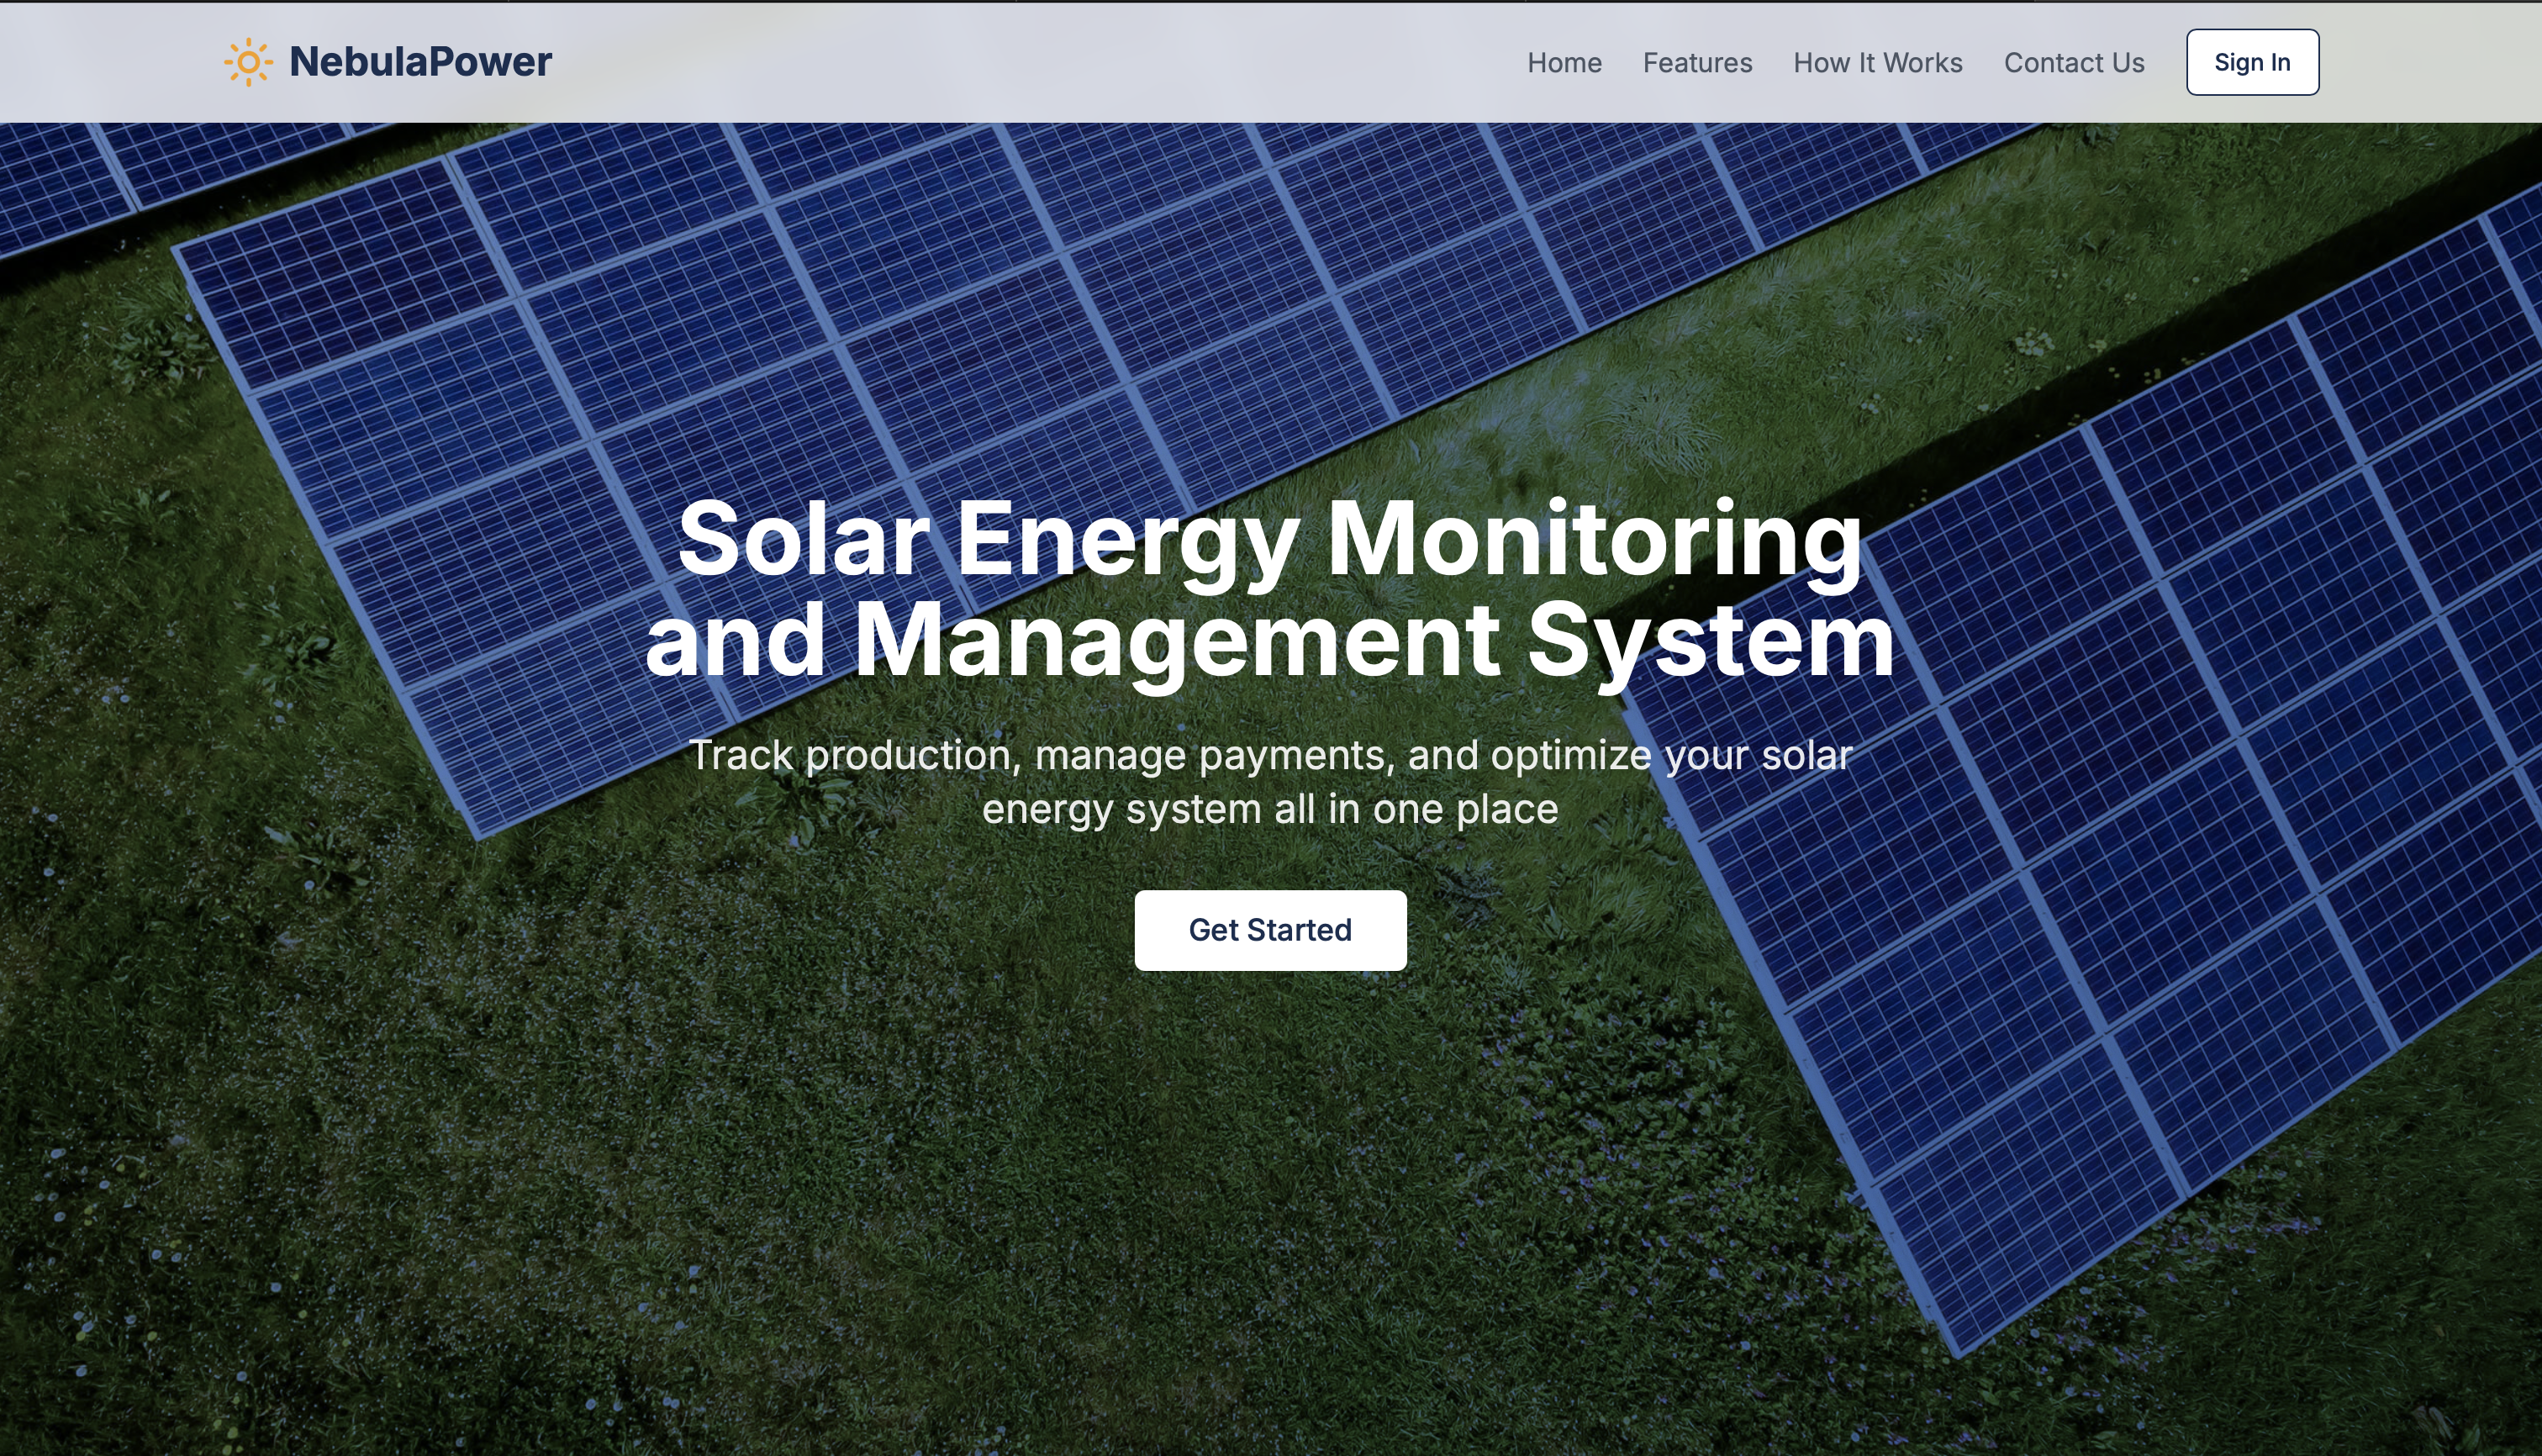
\includegraphics[width=1.1\textwidth]{images_2/landing_page.png}
    \caption{Solar Energy Monitoring and Control System platform landing page}
    \label{fig:architecture}
\end{figure}

\section{Thesis Structure}
\label{sec:structure}

This thesis is organized into the following chapters:

\begin{itemize}
    \item \textbf{Chapter 1: Introduction} - Provides the context, motivation, and high-level overview of the Solar Energy Monitoring and Control System platform.
    
    \item \textbf{Chapter 2: User Documentation} - Detailed documentation for end-users, including installation guides, user interfaces, and operational procedures.
    
    \item \textbf{Chapter 3: Developer Documentation} - Technical documentation covering system architecture, implementation details, APIs, and development guidelines.
\end{itemize}

Each chapter is designed to provide comprehensive information for its target audience, whether they are end-users interacting with the system or developers extending or maintaining the platform.

\chapter{User Documentation}
\label{ch:user}

This chapter provides comprehensive documentation for users of the Solar Energy Monitoring and Control System. The documentation is organized to help different user types quickly find the information they need.

\section{System Overview}
\label{sec:system-overview}

\subsection{What is the Solar Energy Monitoring and Control System?}
\label{subsec:system-description}

The Solar Energy Monitoring and Control System is a web-based platform that enables real-time monitoring and management of solar installations using Pay-As-You-Go (PAYG) financing models. Key capabilities include: real-time energy production and consumption tracking with automated summaries, flexible installment payment management with multiple frequency options, tamper detection and security monitoring, remote service control for payment compliance, role-based user access (Admin/Customer), and comprehensive analytics dashboards.

\subsection{Who Should Use This Documentation}
\label{subsec:target-audience}

\textbf{Primary Users:} System Administrators (platform configuration, user management) and Solar Installation Customers (energy monitoring, payment management).

\textbf{Prerequisites:} Administrators need web application management skills; Customers need basic computer literacy and email access.

\subsection{System Components}
\label{subsec:system-components}

The system consists of four main components: (1) \textbf{Backend API} -- Spring Boot application providing REST APIs, WebSocket endpoints for real-time updates, business logic, and authentication; (2) \textbf{Frontend Web Application} -- Next.js-based responsive interface with separate dashboards for administrators and customers; (3) \textbf{PostgreSQL Database} -- Stores user data, energy readings, payments, tamper events, and operational logs; (4) \textbf{IoT Device/Simulator} -- Python-based component representing Raspberry Pi devices installed at solar sites to collect and transmit energy data and tamper alerts (simulator provided for testing without physical hardware). The system implements role-based access control with two roles (Table~\ref{tab:role-privileges}).

\begin{table}[h]
    \centering
    \caption{Access privileges by user role}
    \label{tab:role-privileges}
    \begin{tabular}{|l|c|c|}
        \hline
        \textbf{Feature} & \textbf{Admin} & \textbf{Customer} \\
        \hline
        User Management & Full & Self Only \\
        Energy Monitoring & Full & Own Only \\
        Payment Processing & Full & Own Only \\
        Security Alerts & Full & Limited \\
        System Configuration & Full & No \\
        Reports & Full & Limited \\
        \hline
    \end{tabular}
\end{table}

\section{Quick Start Guide}
\label{sec:quick-start}

\subsection{System Requirements}
\label{subsec:system-requirements}

\subsubsection{For End Users (Customers)}
\label{subsubsec:end-user-requirements}

Requirements: Modern computer/tablet/smartphone, stable internet (1+ Mbps), active email account. Supported browsers: Chrome 88+, Firefox 85+, Edge 88+, Safari 14+. JavaScript and cookies must be enabled. Minimum resolution: 1280$\times$768.

\subsubsection{For System Administrators}
\label{subsubsec:admin-requirements}

Since the system runs in Docker containers, administrators only need Docker Desktop (or Docker Engine with Docker Compose) installed on their host system. Recommended hardware: at least 8GB RAM and sufficient disk space for container images and database storage. All other dependencies (Java, PostgreSQL, etc.) are bundled within the containers.

\subsection{Account Access}
\label{subsec:account-access}

\subsubsection{Getting Your Account}
\label{subsubsec:getting-account}

\textbf{For Customers:} Your solar installation provider (administrator) will create your account and you will receive an email with an activation link. Click the link, then set your password following the requirements: minimum 8 characters including at least one uppercase letter, one lowercase letter, one number, and one special character.

\textbf{For Administrators:} The administrator account is automatically created during system deployment using credentials configured in the environment file. On first login, you must change this default password to a secure one.

\subsubsection{Logging In}
\label{subsubsec:logging-in}

Navigate to system URL, enter email and password, click "Sign In". Figure~\ref{fig:login} shows the login interface.

\begin{figure}[htbp]
    \centering
    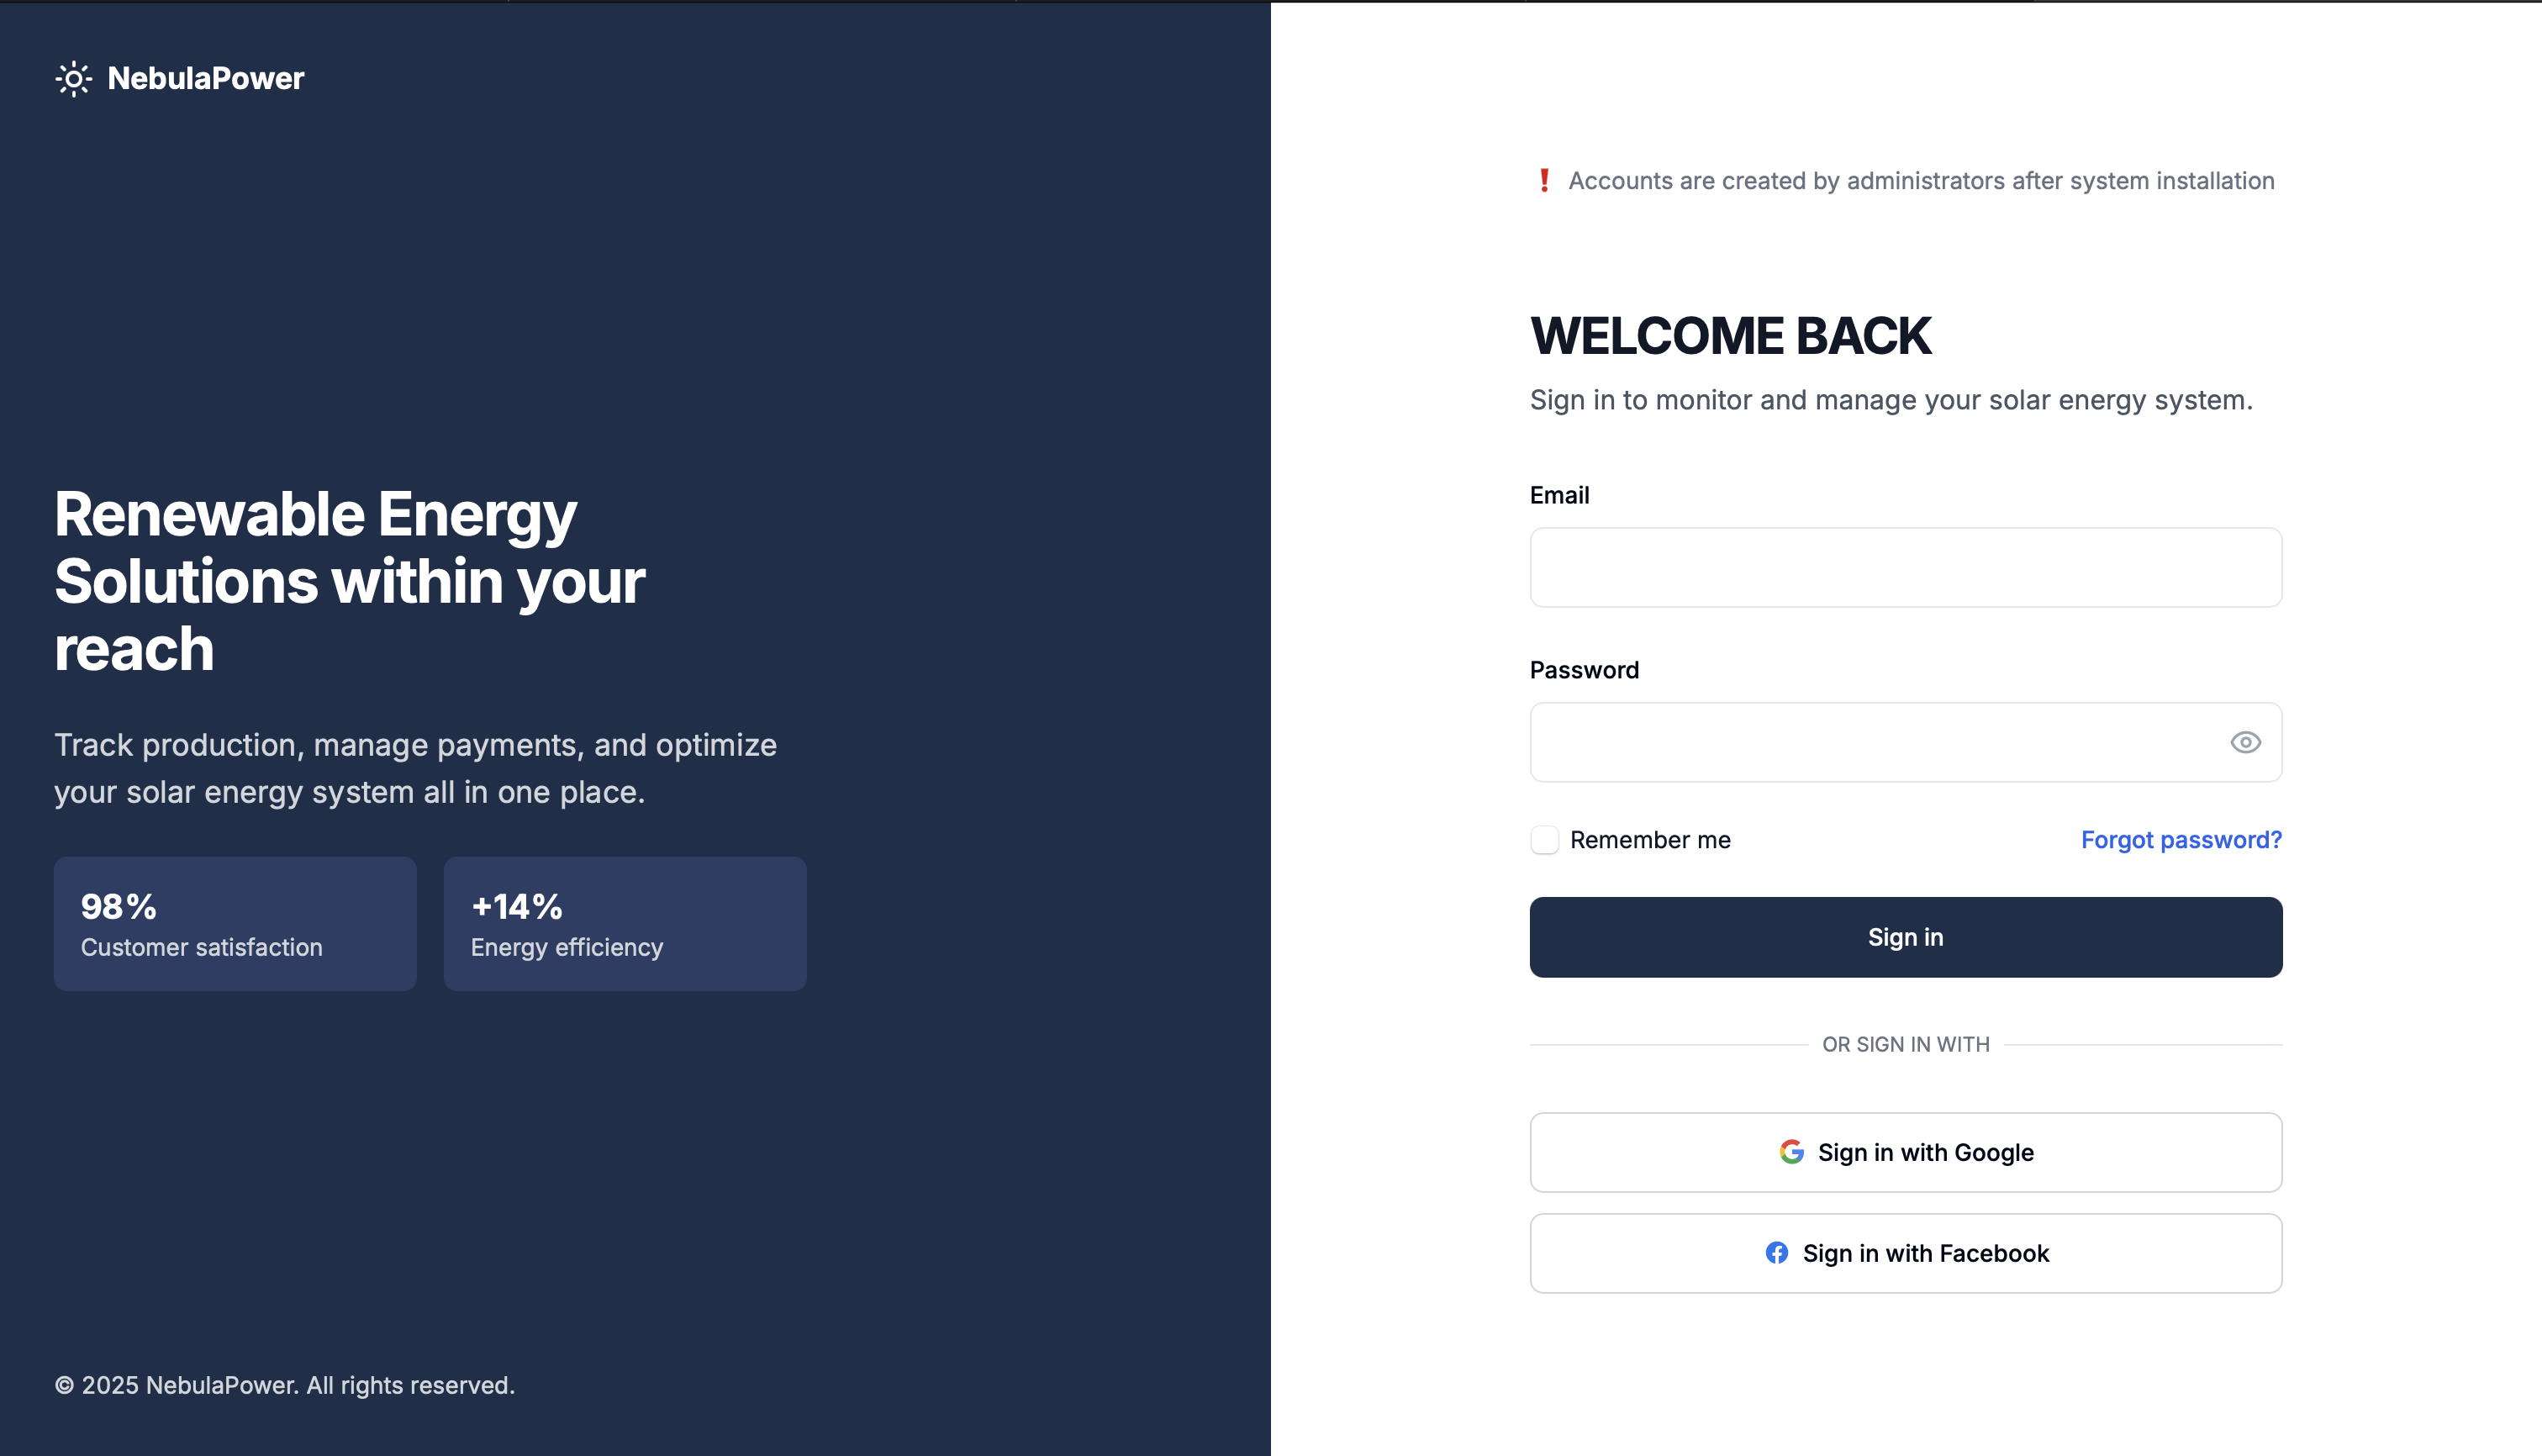
\includegraphics[width=0.9\textwidth]{images_2/login_pg.png}
    \caption{User login interface}
    \label{fig:login}
\end{figure}

\subsubsection{Password Management}
\label{subsubsec:password-management}

\textbf{Note}: Email functionality is simulated for demonstration only.

\textbf{Reset:} Click "Forgot Password," enter email, follow reset link. \textbf{Change:} Profile Settings $\rightarrow$ enter current and new passwords $\rightarrow$ save.

\section{User Interface Guide}
\label{sec:ui-guide}

\subsection{Technical Requirements}

The web interface works with modern browsers including Chrome, Firefox, Edge, Safari, and Opera. You need JavaScript and cookies enabled, and a screen resolution of at least 1280$\times$768 pixels. A stable internet connection is required for accessing the system and receiving real-time updates.

\section{Installation and Setup Guide}
\label{sec:installation-setup}

\subsection{Prerequisites}
\label{subsec:prerequisites}

Before installing, ensure you have Docker Desktop (version 4.0 or newer) or Docker Engine (version 20.10 or newer) with Docker Compose (version 2.0 or newer) installed on your system. Your computer should have at least 4GB of RAM available, though 8GB is recommended for better performance.

\subsection{Quick Docker Installation}
\label{subsec:docker-installation}

\textbf{1) Clone and prepare environment}

Open a terminal or command-line interface and navigate to the folder where you want to install the system, then run:

\begin{verbatim}
git clone https://github.com/2001J/nebular-power.git
cd nebular-power
cp .env.template .env     # create .env (copied from .env.template)
\end{verbatim}

Open the \texttt{.env} file and set your administrator credentials (\texttt{ADMIN\_EMAIL}, \texttt{ADMIN\_PASSWORD}) and a secure random string for \texttt{JWT\_SECRET}. The database settings have sensible defaults that you can change if needed.

\textbf{2) Start services}
\begin{verbatim}
docker compose up -d
\end{verbatim}

This command starts three containers running the database, backend API, and frontend application. Wait a minute or two for the database to initialize.

\textbf{3) Access the application}
\begin{itemize}
    \item Web Interface: \url{http://localhost:3000}
    \item API Documentation: \url{http://localhost:8080/swagger-ui.html}
\end{itemize}

Log in using the administrator credentials you configured. You should change the password on first login for security.

\subsection{Configuration}
\label{subsec:system-configuration}

All system settings are managed through the \texttt{.env} file (copied from \texttt{.env.template}). The most important settings include your administrator account details for initial access, authentication secrets for security, database connection settings (with defaults provided), email server configuration for notifications (optional for local testing), and the system profile which determines whether to use the development or production database.

For production deployment, use strong passwords and secrets, and configure a real email service for sending notifications.

\subsection{Device Simulation}
\label{subsec:device-simulation}

To simulate IoT devices sending energy data and tamper alerts, you need to set up the Python simulator. This can run on the same machine as your Docker containers (using \texttt{localhost:8080} as the backend URL) or on a separate device like a Raspberry Pi (using the IP address of the machine running the backend).

\textbf{Setup steps:}

Navigate to the simulation folder and create a virtual environment:
\begin{verbatim}
cd pi_simulation
python3 -m venv venv
source venv/bin/activate      # On Windows: venv\Scripts\activate
\end{verbatim}

Install dependencies:
\begin{verbatim}
pip3 install -r requirements.txt
\end{verbatim}

Edit \texttt{config.json} to set the backend URL:
\begin{itemize}
    \item For same machine: \texttt{http://localhost:8080}
    \item For Raspberry Pi or separate device: \texttt{http://[BACKEND\_IP]:8080} (replace \texttt{[BACKEND\_IP]} with the actual IP address)
\end{itemize}

Run the simulator:
\begin{verbatim}
python3 main.py
\end{verbatim}

\subsection{Verification and Management}
\label{subsec:verification}

After installation, verify everything is running by checking container status with \texttt{docker compose ps}. You can view logs using \texttt{docker compose logs -f backend} to monitor the application. Open the web interface and sign in with your administrator credentials to confirm successful deployment.

If you encounter port conflicts, adjust the \texttt{POSTGRES\_HOST\_PORT} setting in your \texttt{.env} file. If the database takes time to initialize, wait 2--3 minutes and check the database logs with \texttt{docker compose logs postgres}. For authentication issues, verify that your database credentials in \texttt{.env} match correctly.

To manage the system, use \texttt{docker compose up -d} to start services, \texttt{docker compose down} to stop everything, \texttt{docker compose restart backend} to restart a specific service, and \texttt{docker compose logs -f backend} to monitor logs in real-time.

\subsection{Account Setup and Access}
\label{subsec:account-setup}

Administrators can create customer accounts through the Customer Management interface. New customers receive an activation email and set their own password following security requirements (minimum 8 characters with uppercase, lowercase, numbers, and special characters). See Figure~\ref{fig:customer-onboarding}.

\begin{figure}[htbp]
    \centering
    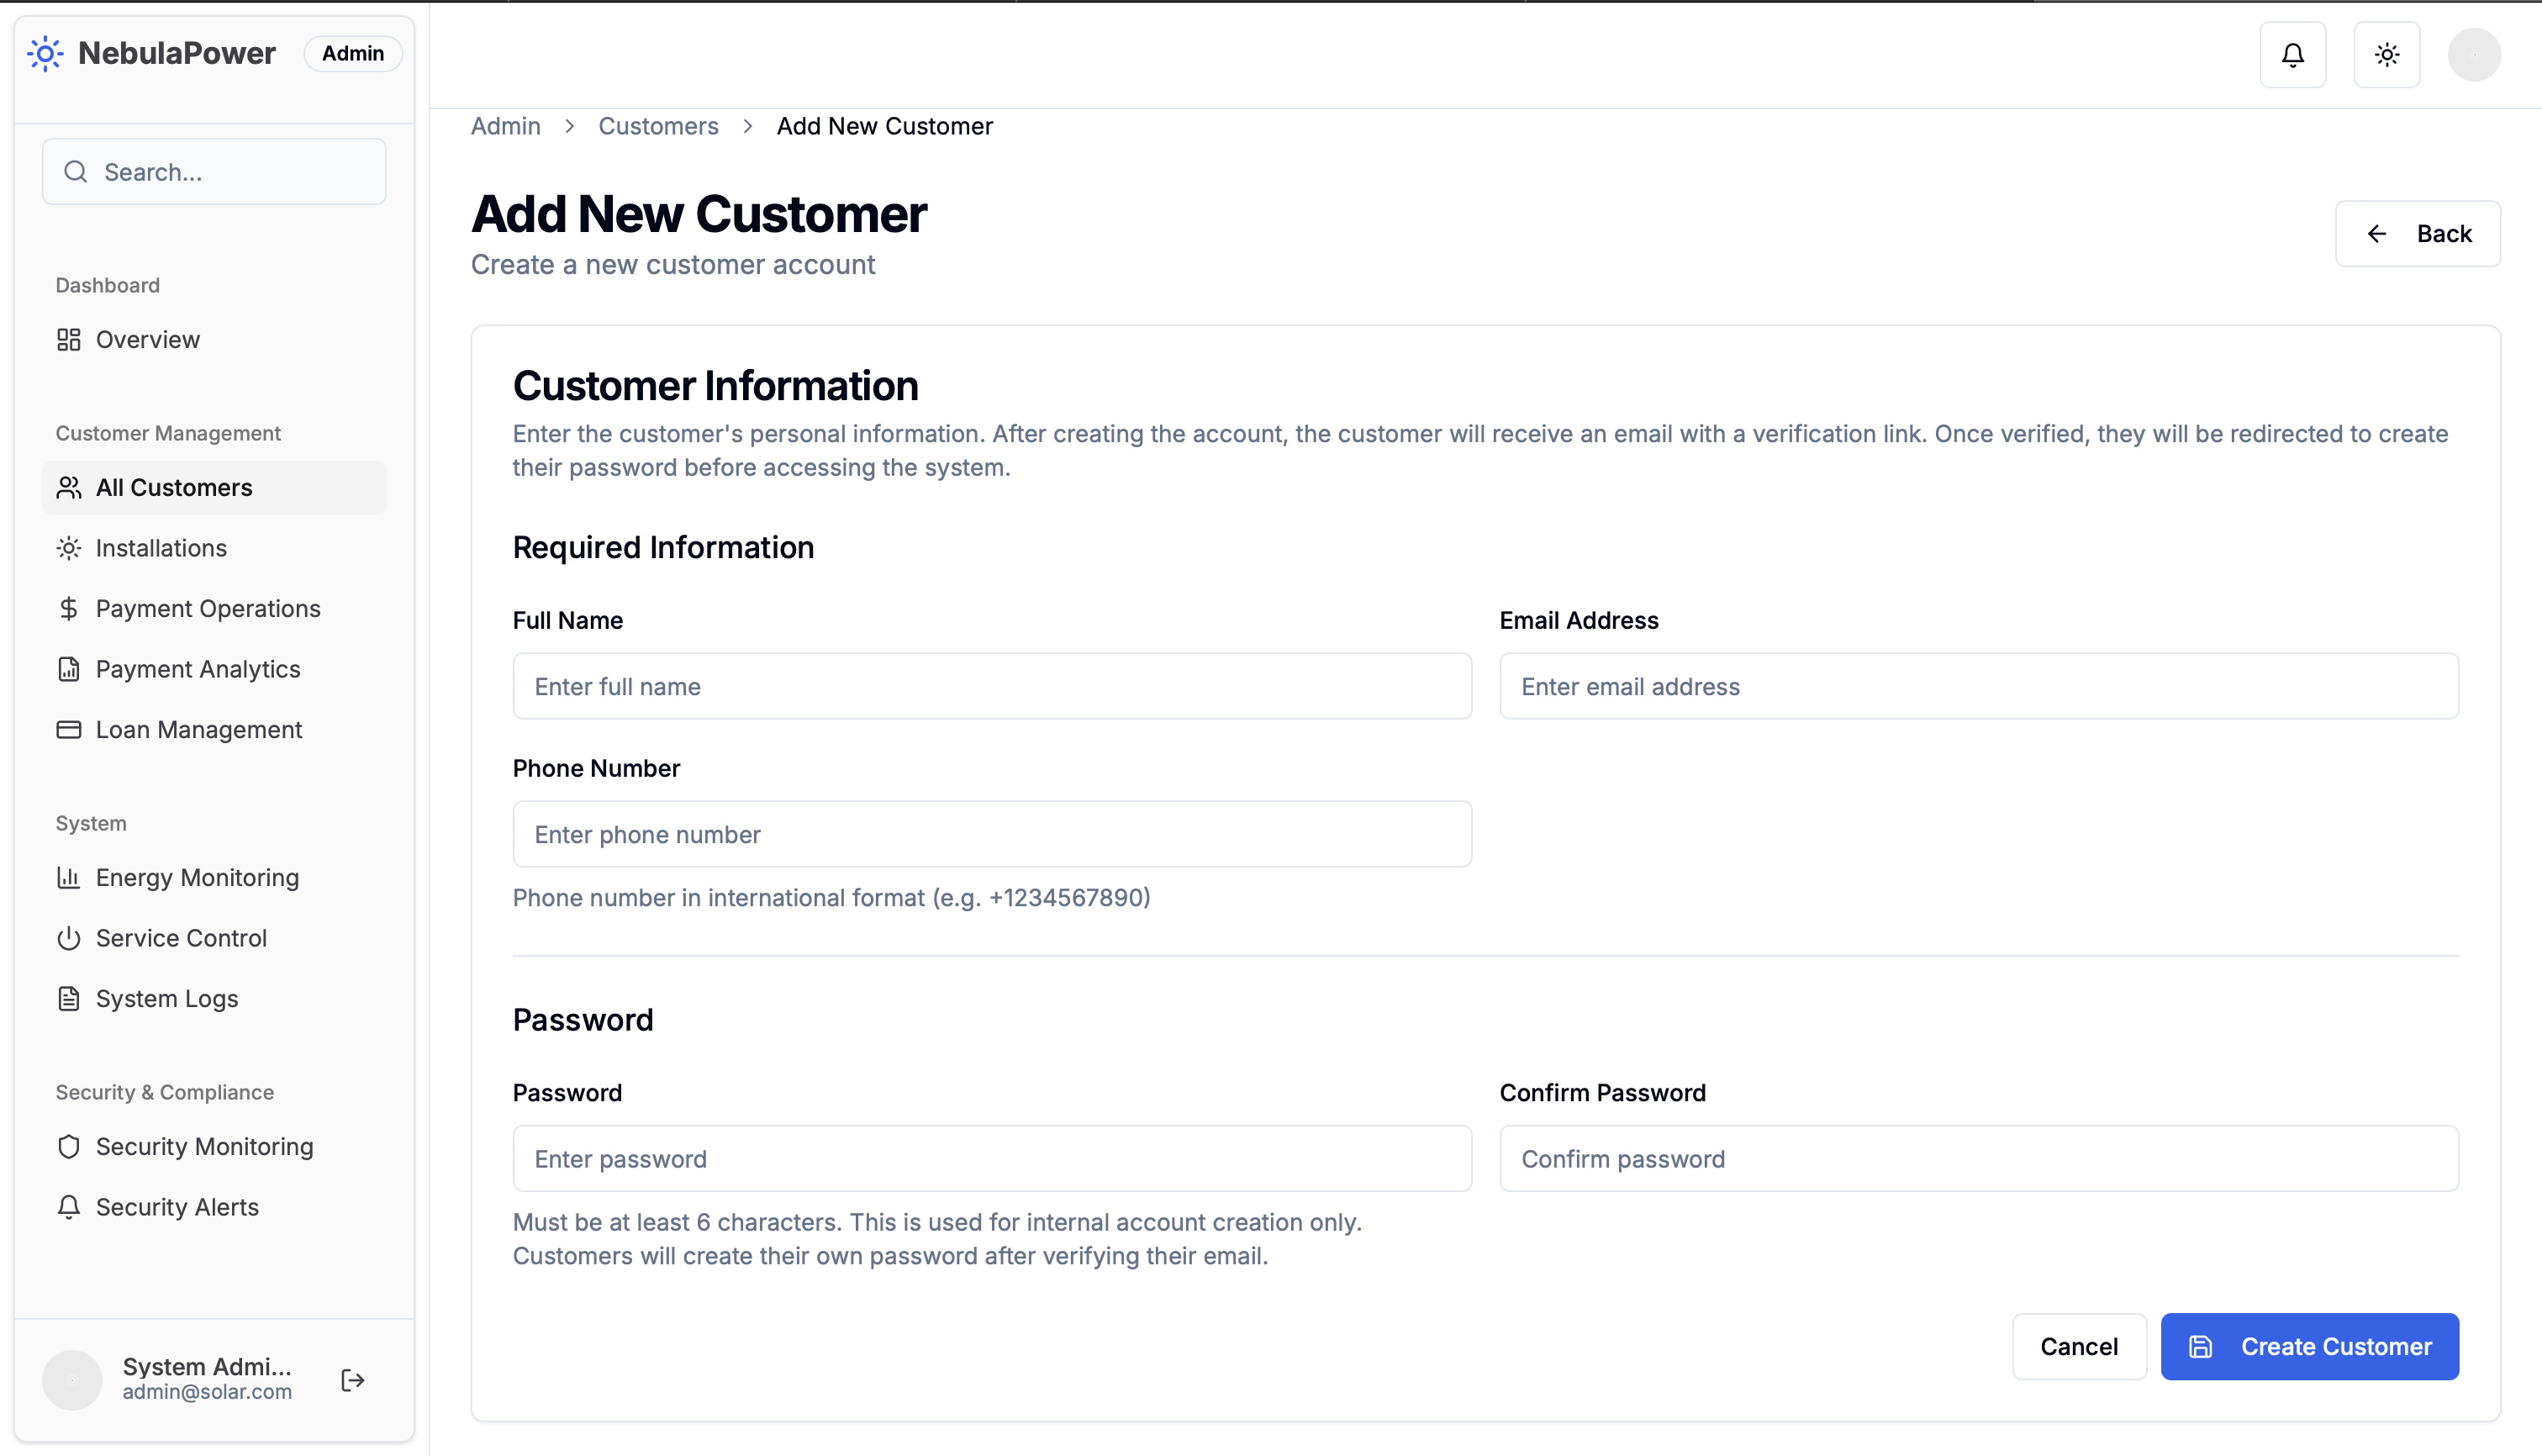
\includegraphics[width=0.9\textwidth]{images_2/customer_onboard.png}
    \caption{Customer onboarding interface (admin view)}
    \label{fig:customer-onboarding}
\end{figure}

\textbf{Login:} Navigate to login page, enter email/password, click "Sign In."

\textbf{Password Management:} Reset via "Forgot Password" link; change in profile settings.

\section{Dashboard Interface Guide}
\label{sec:dashboard-guide}

This section provides a detailed overview of the Solar Energy Monitoring and Control System's user interface, highlighting key screens and navigation patterns.

\subsection{Dashboard Overview}
\label{subsec:dashboard-overview}

The dashboard is your main workspace after logging in. The interface you see depends on your user role.

\subsubsection{Administrator Dashboard}
\label{subsubsec:admin-dashboard}

Navigation: Dashboard (system overview), Customer Management, Payment Operations, System (energy, logs), Security \& Compliance. See Figure~\ref{fig:admin-dashboard}.

\begin{figure}[h]
    \centering
    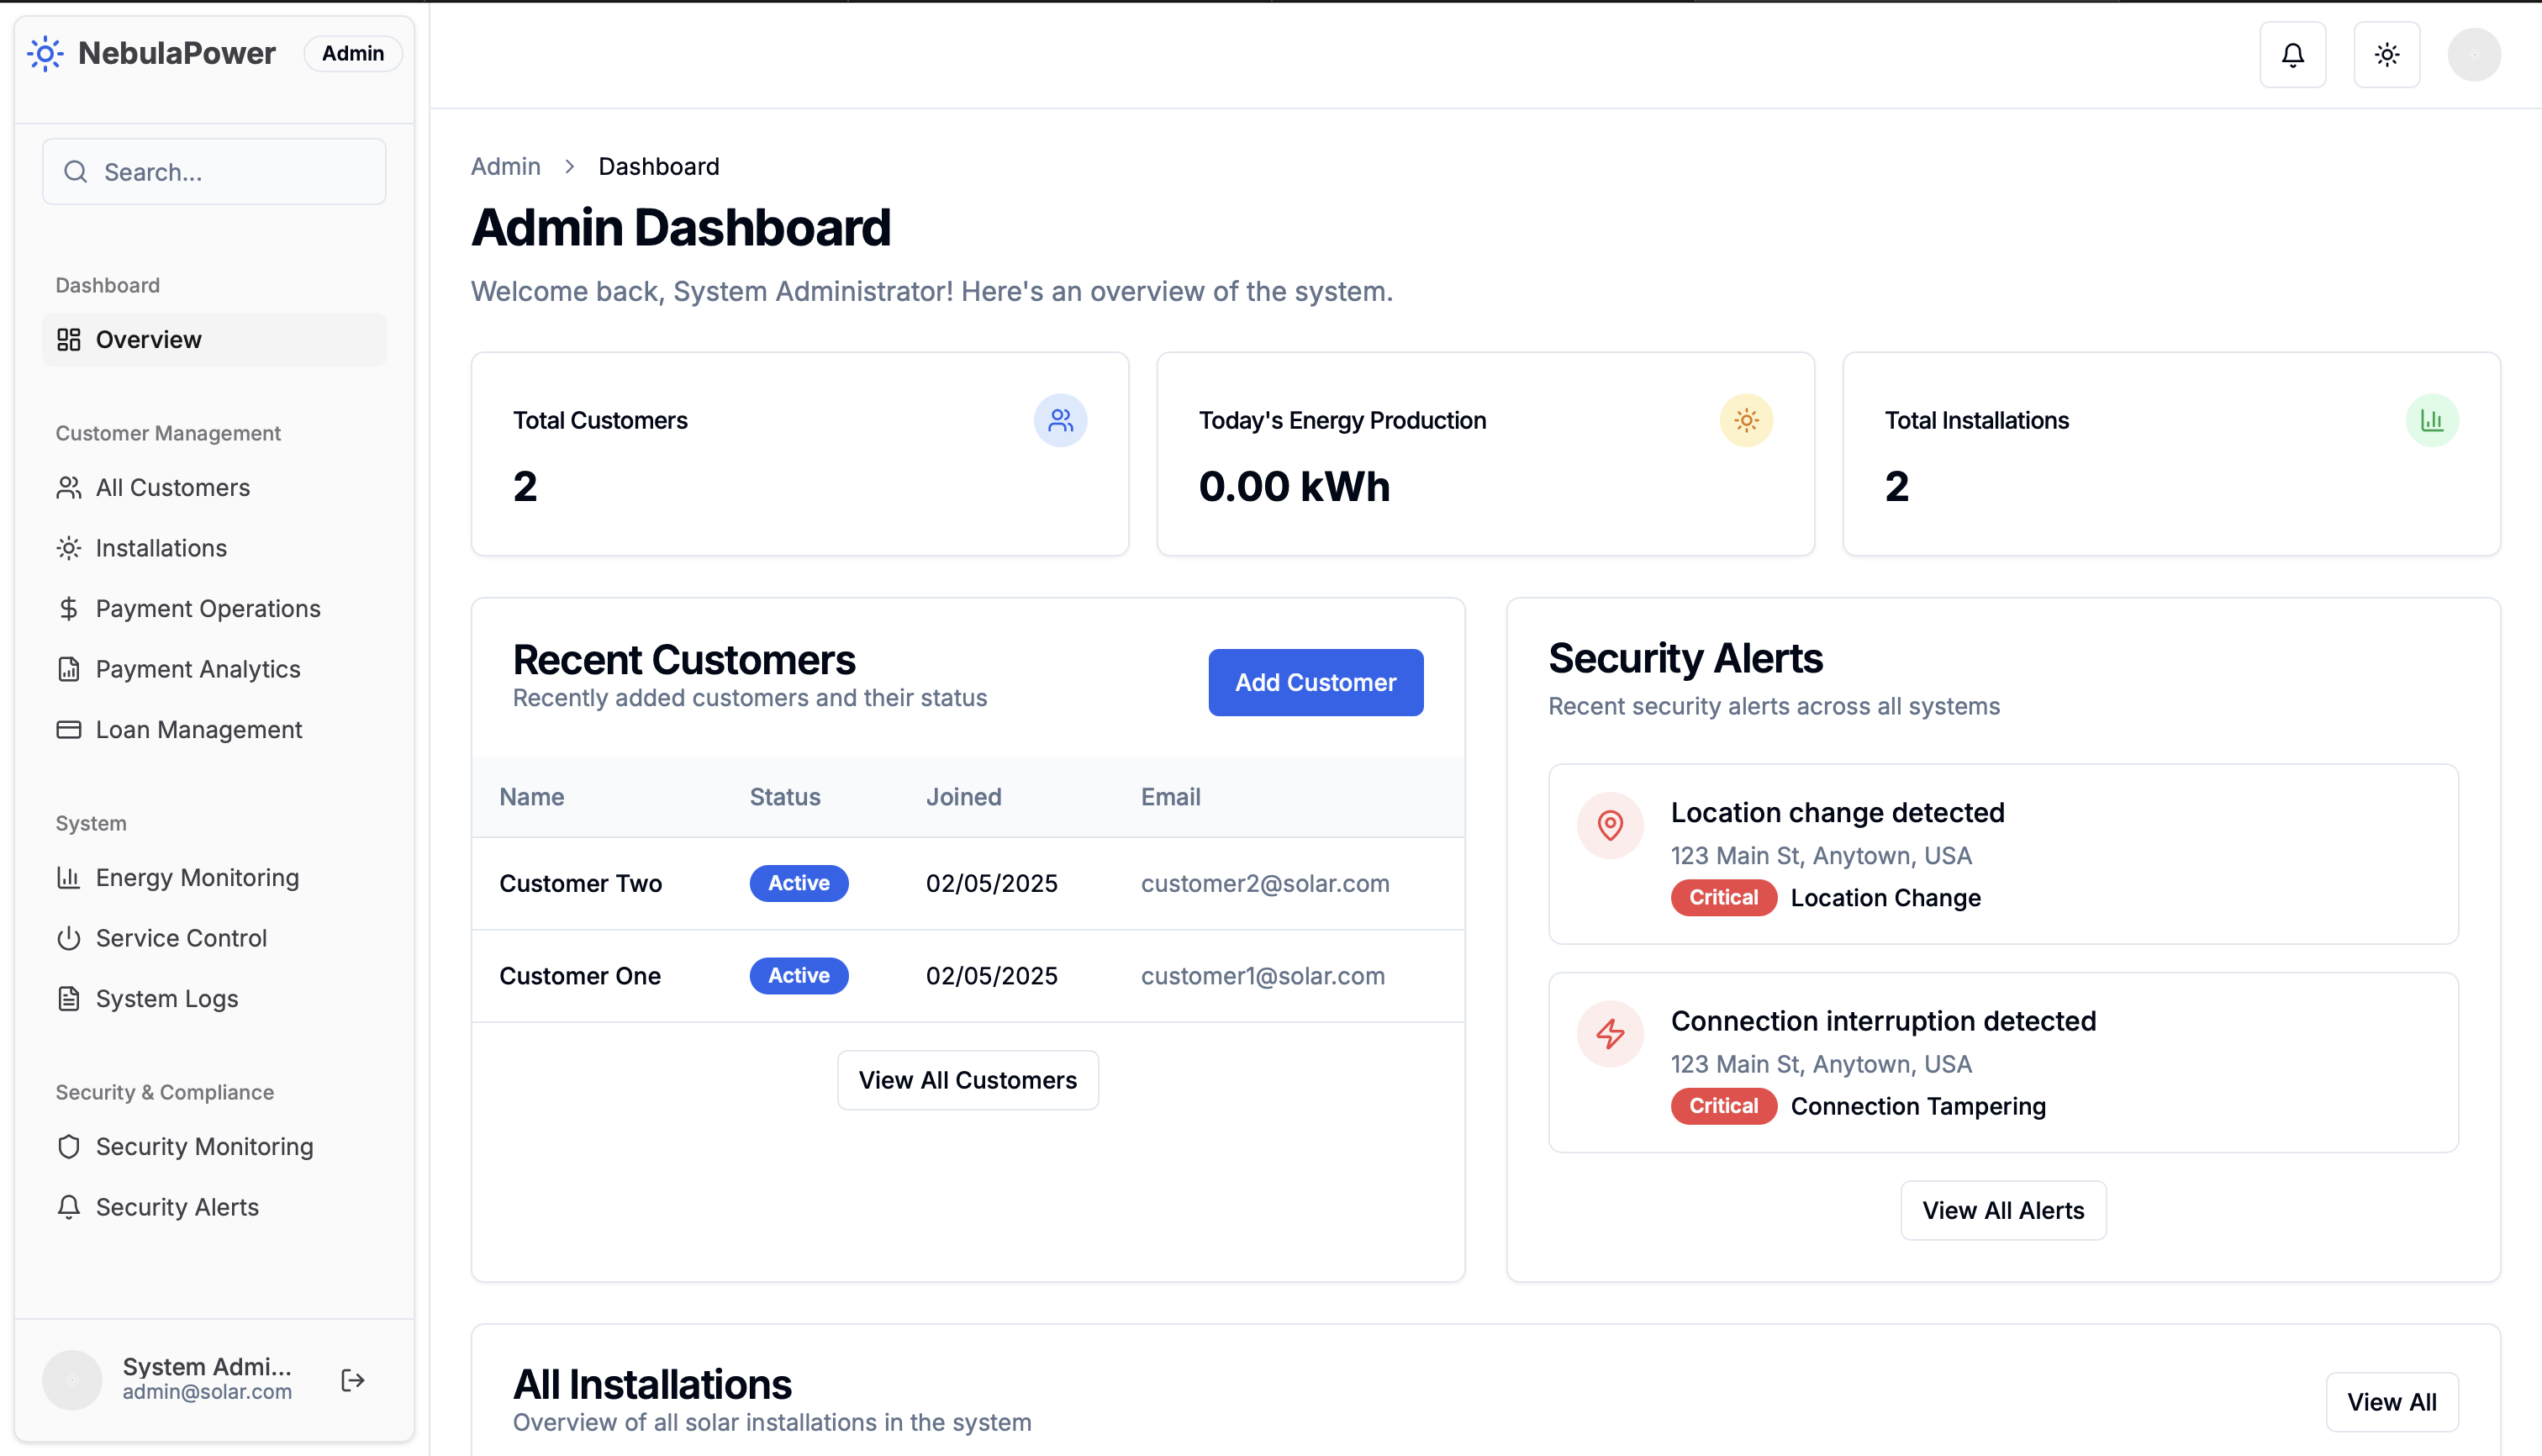
\includegraphics[width=0.9\textwidth]{images_2/admin_dashboard.png}
    \caption{Administrator dashboard}
    \label{fig:admin-dashboard}
\end{figure}

\subsubsection{Customer Dashboard}
\label{subsubsec:customer-dashboard}

Shows installation summary, loan status, payment information, with tabs for Overview, Installations, Payments. See Figure~\ref{fig:customer-dashboard}.

\begin{figure}[h]
    \centering
    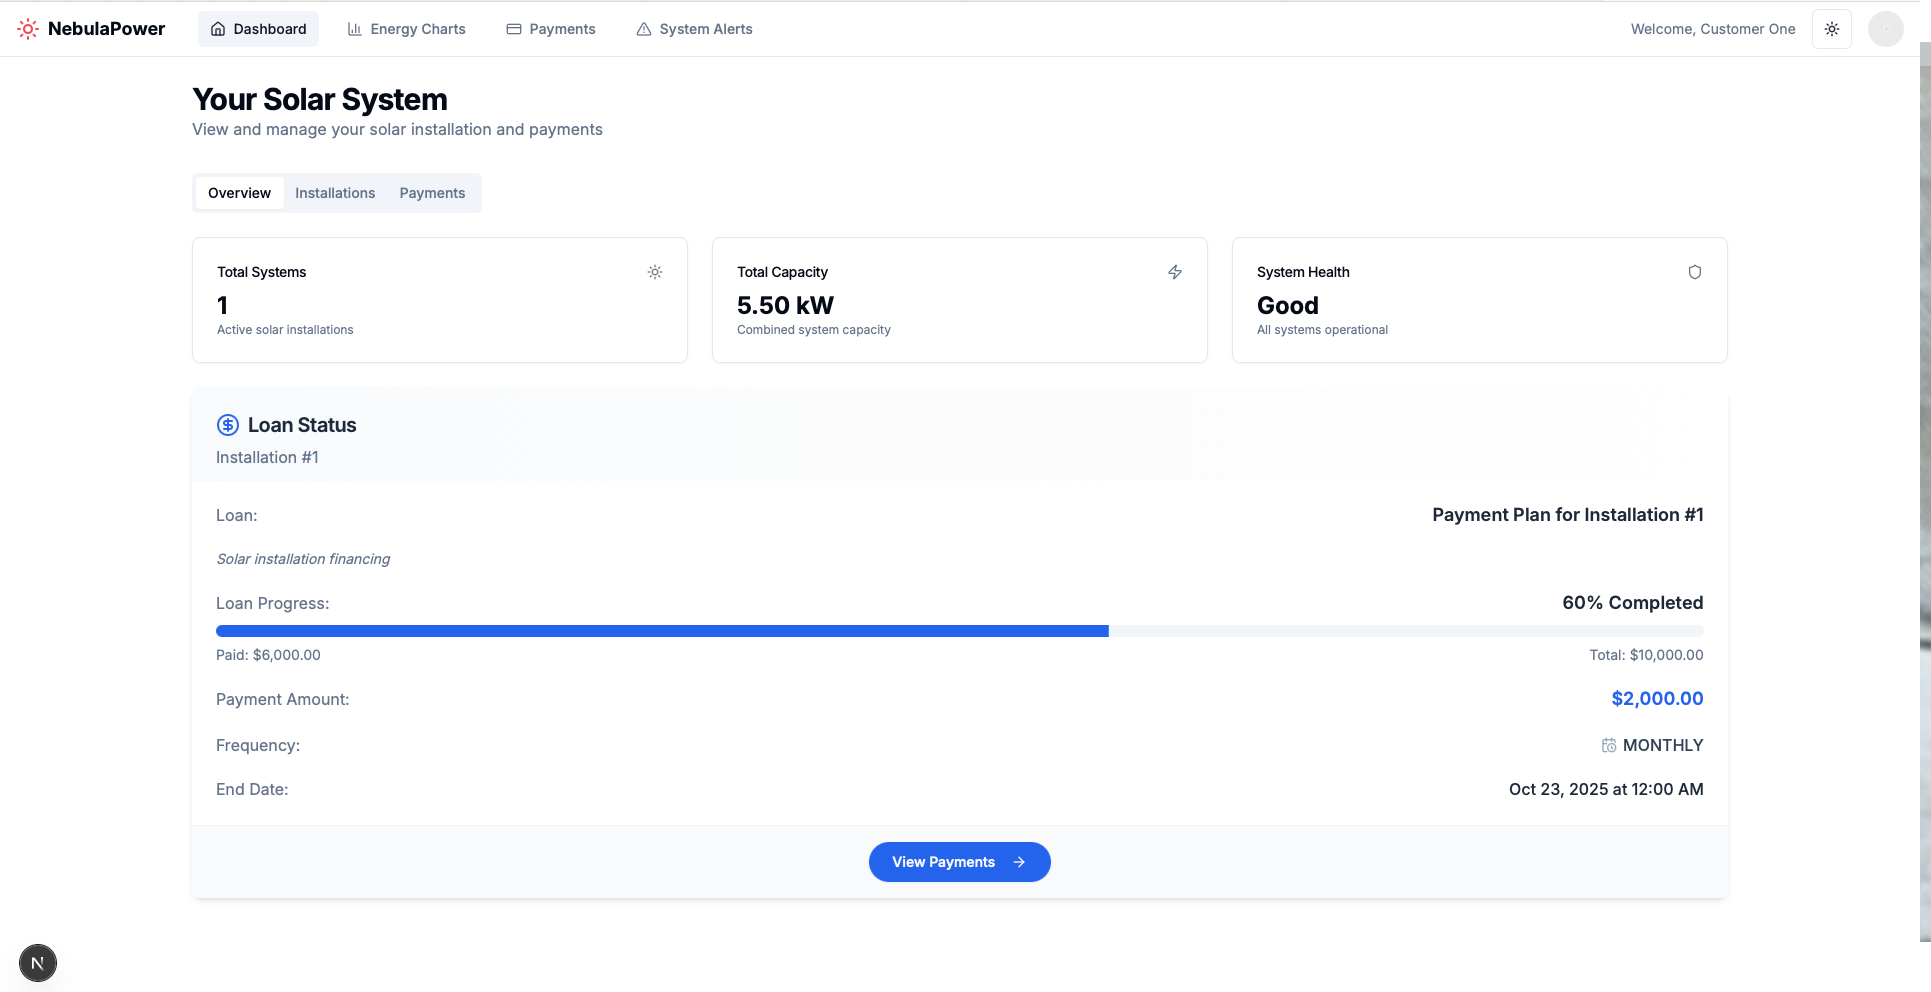
\includegraphics[width=0.9\textwidth]{images_2/customer_dashboard.png}
    \caption{Customer dashboard}
    \label{fig:customer-dashboard}
\end{figure}

\subsection{Energy Monitoring}
\label{subsec:energy-monitoring}

\textbf{Customer View:} Shows current generation, daily/monthly production, efficiency, environmental impact, with production graphs and health indicators (Figure~\ref{fig:customer-energy}).

\begin{figure}[h]
    \centering
    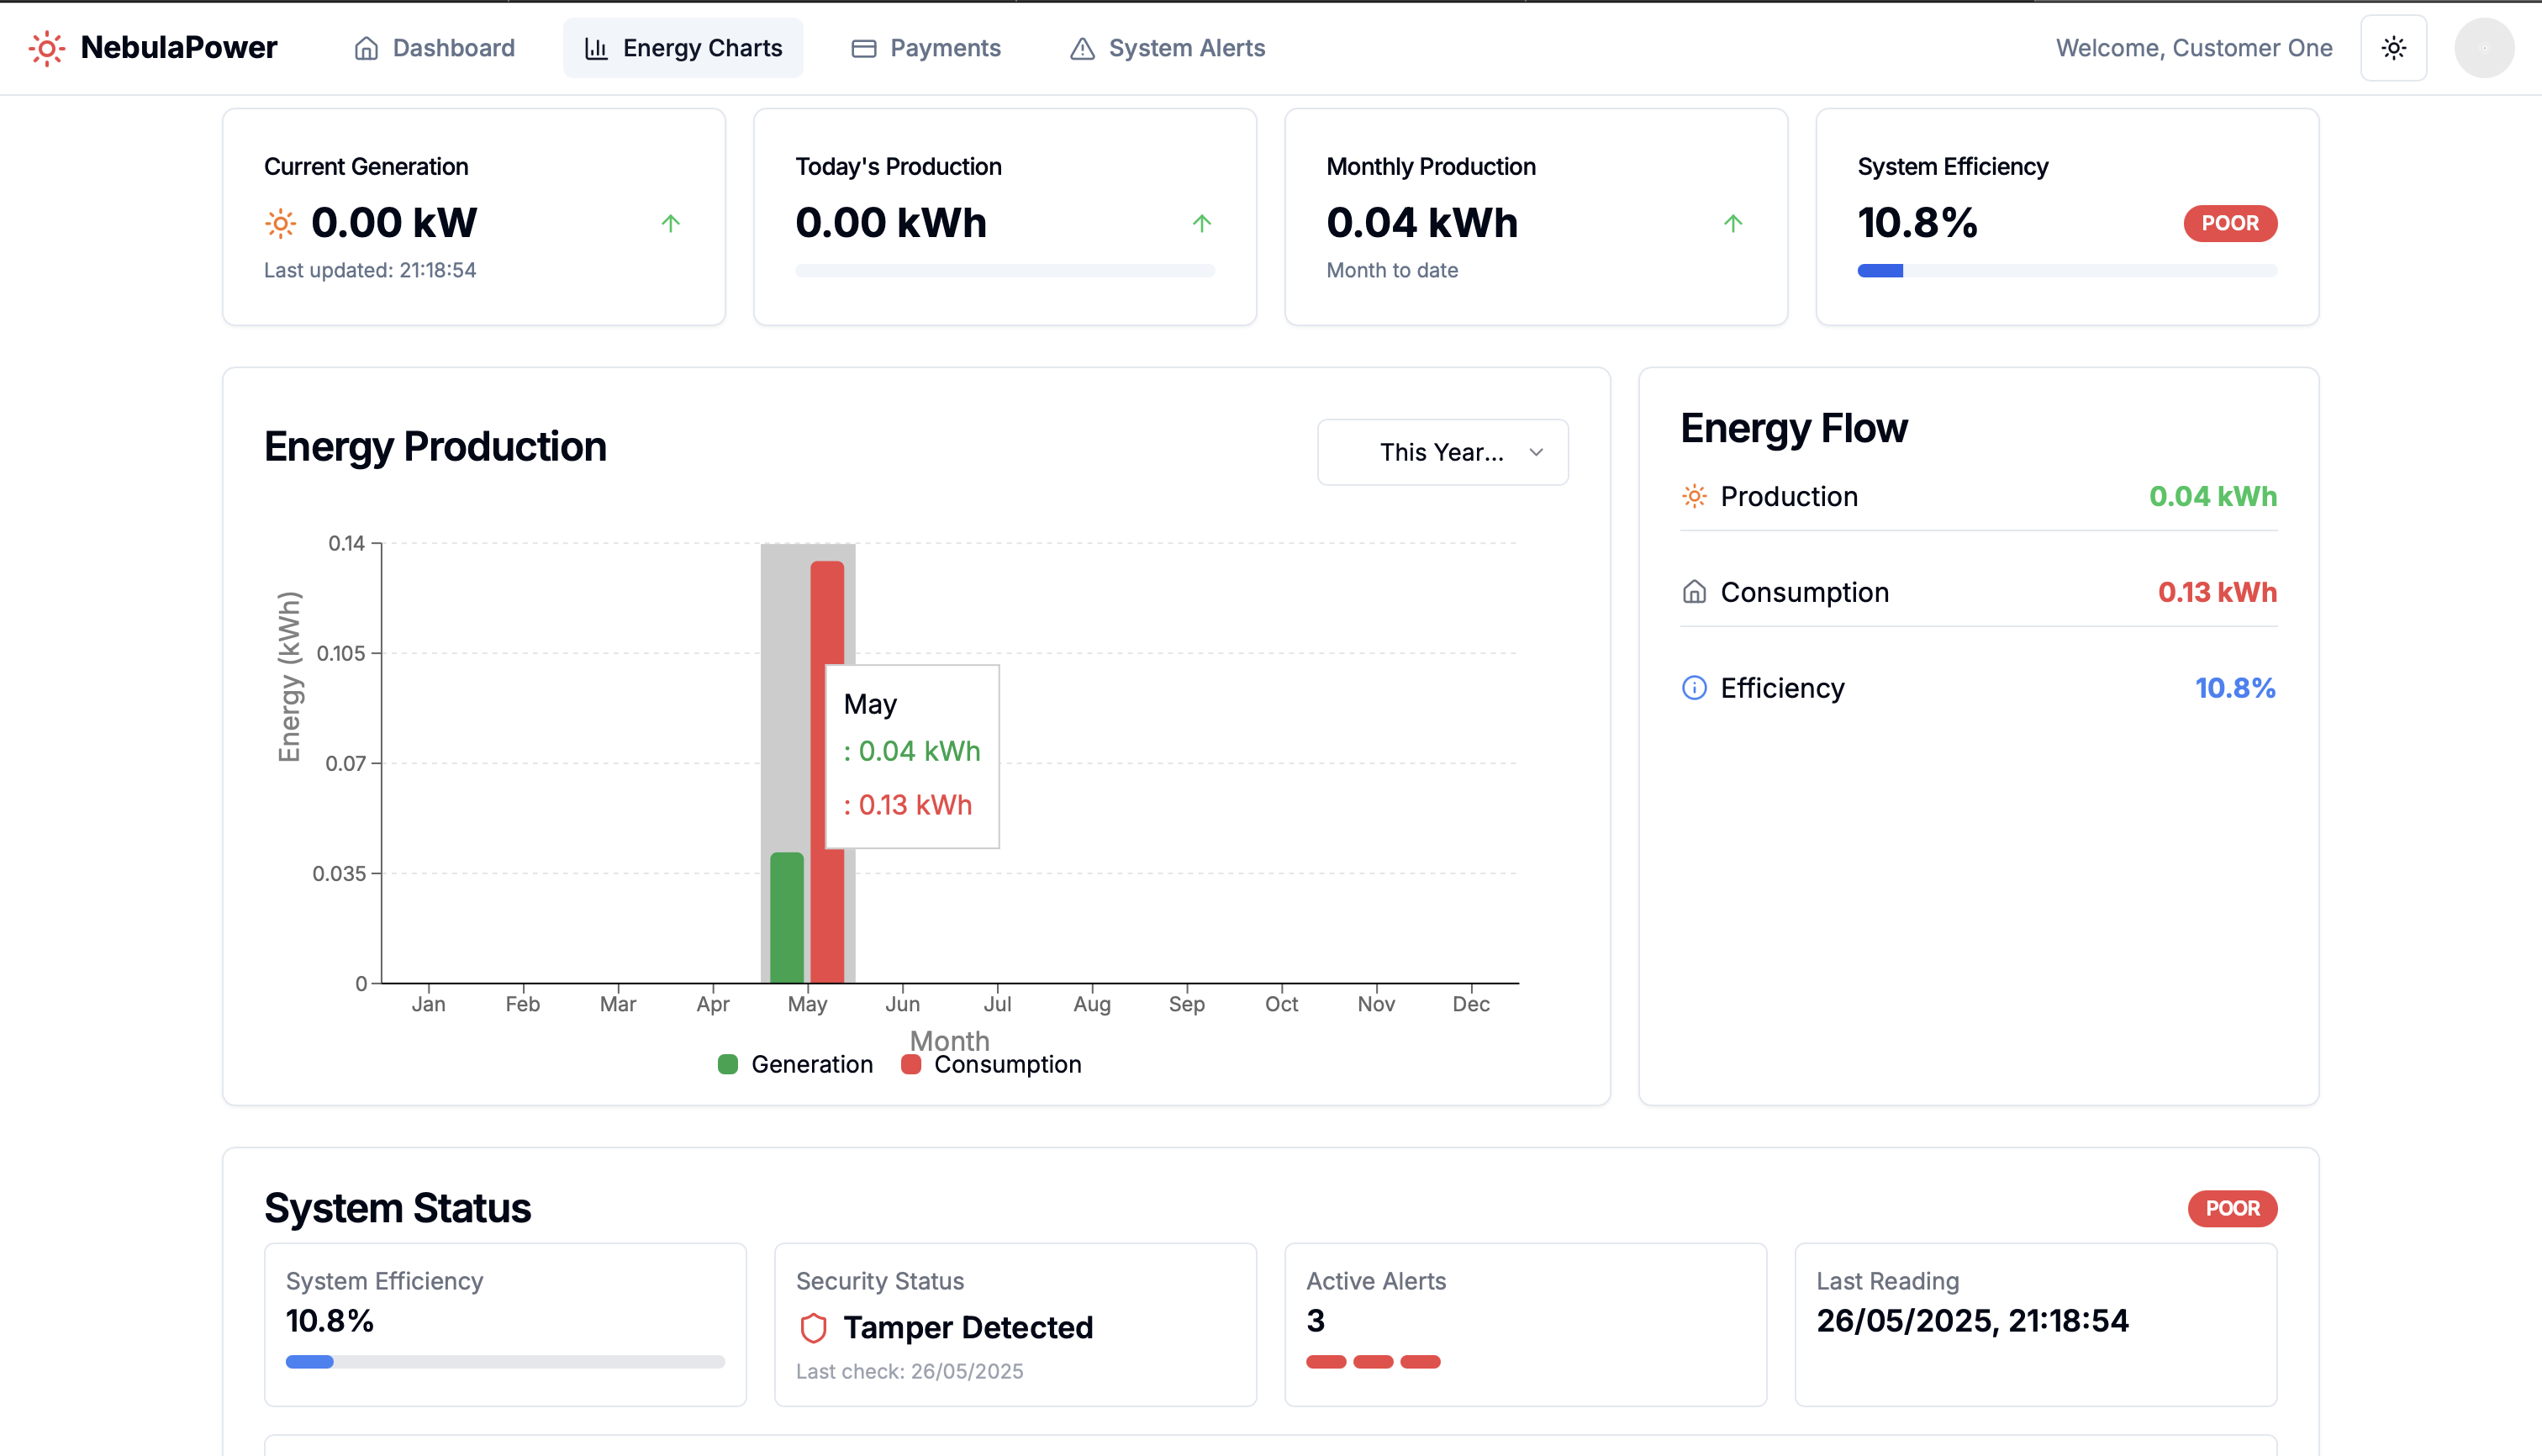
\includegraphics[width=0.85\textwidth]{images_2/customer_energy_dashb.png}
    \caption{Customer energy monitoring dashboard}
    \label{fig:customer-energy}
\end{figure}

\textbf{Admin View:} Displays aggregated metrics, installation comparisons, performance rankings, status indicators across all systems (Figure~\ref{fig:admin-energy}).

\begin{figure}[h]
    \centering
    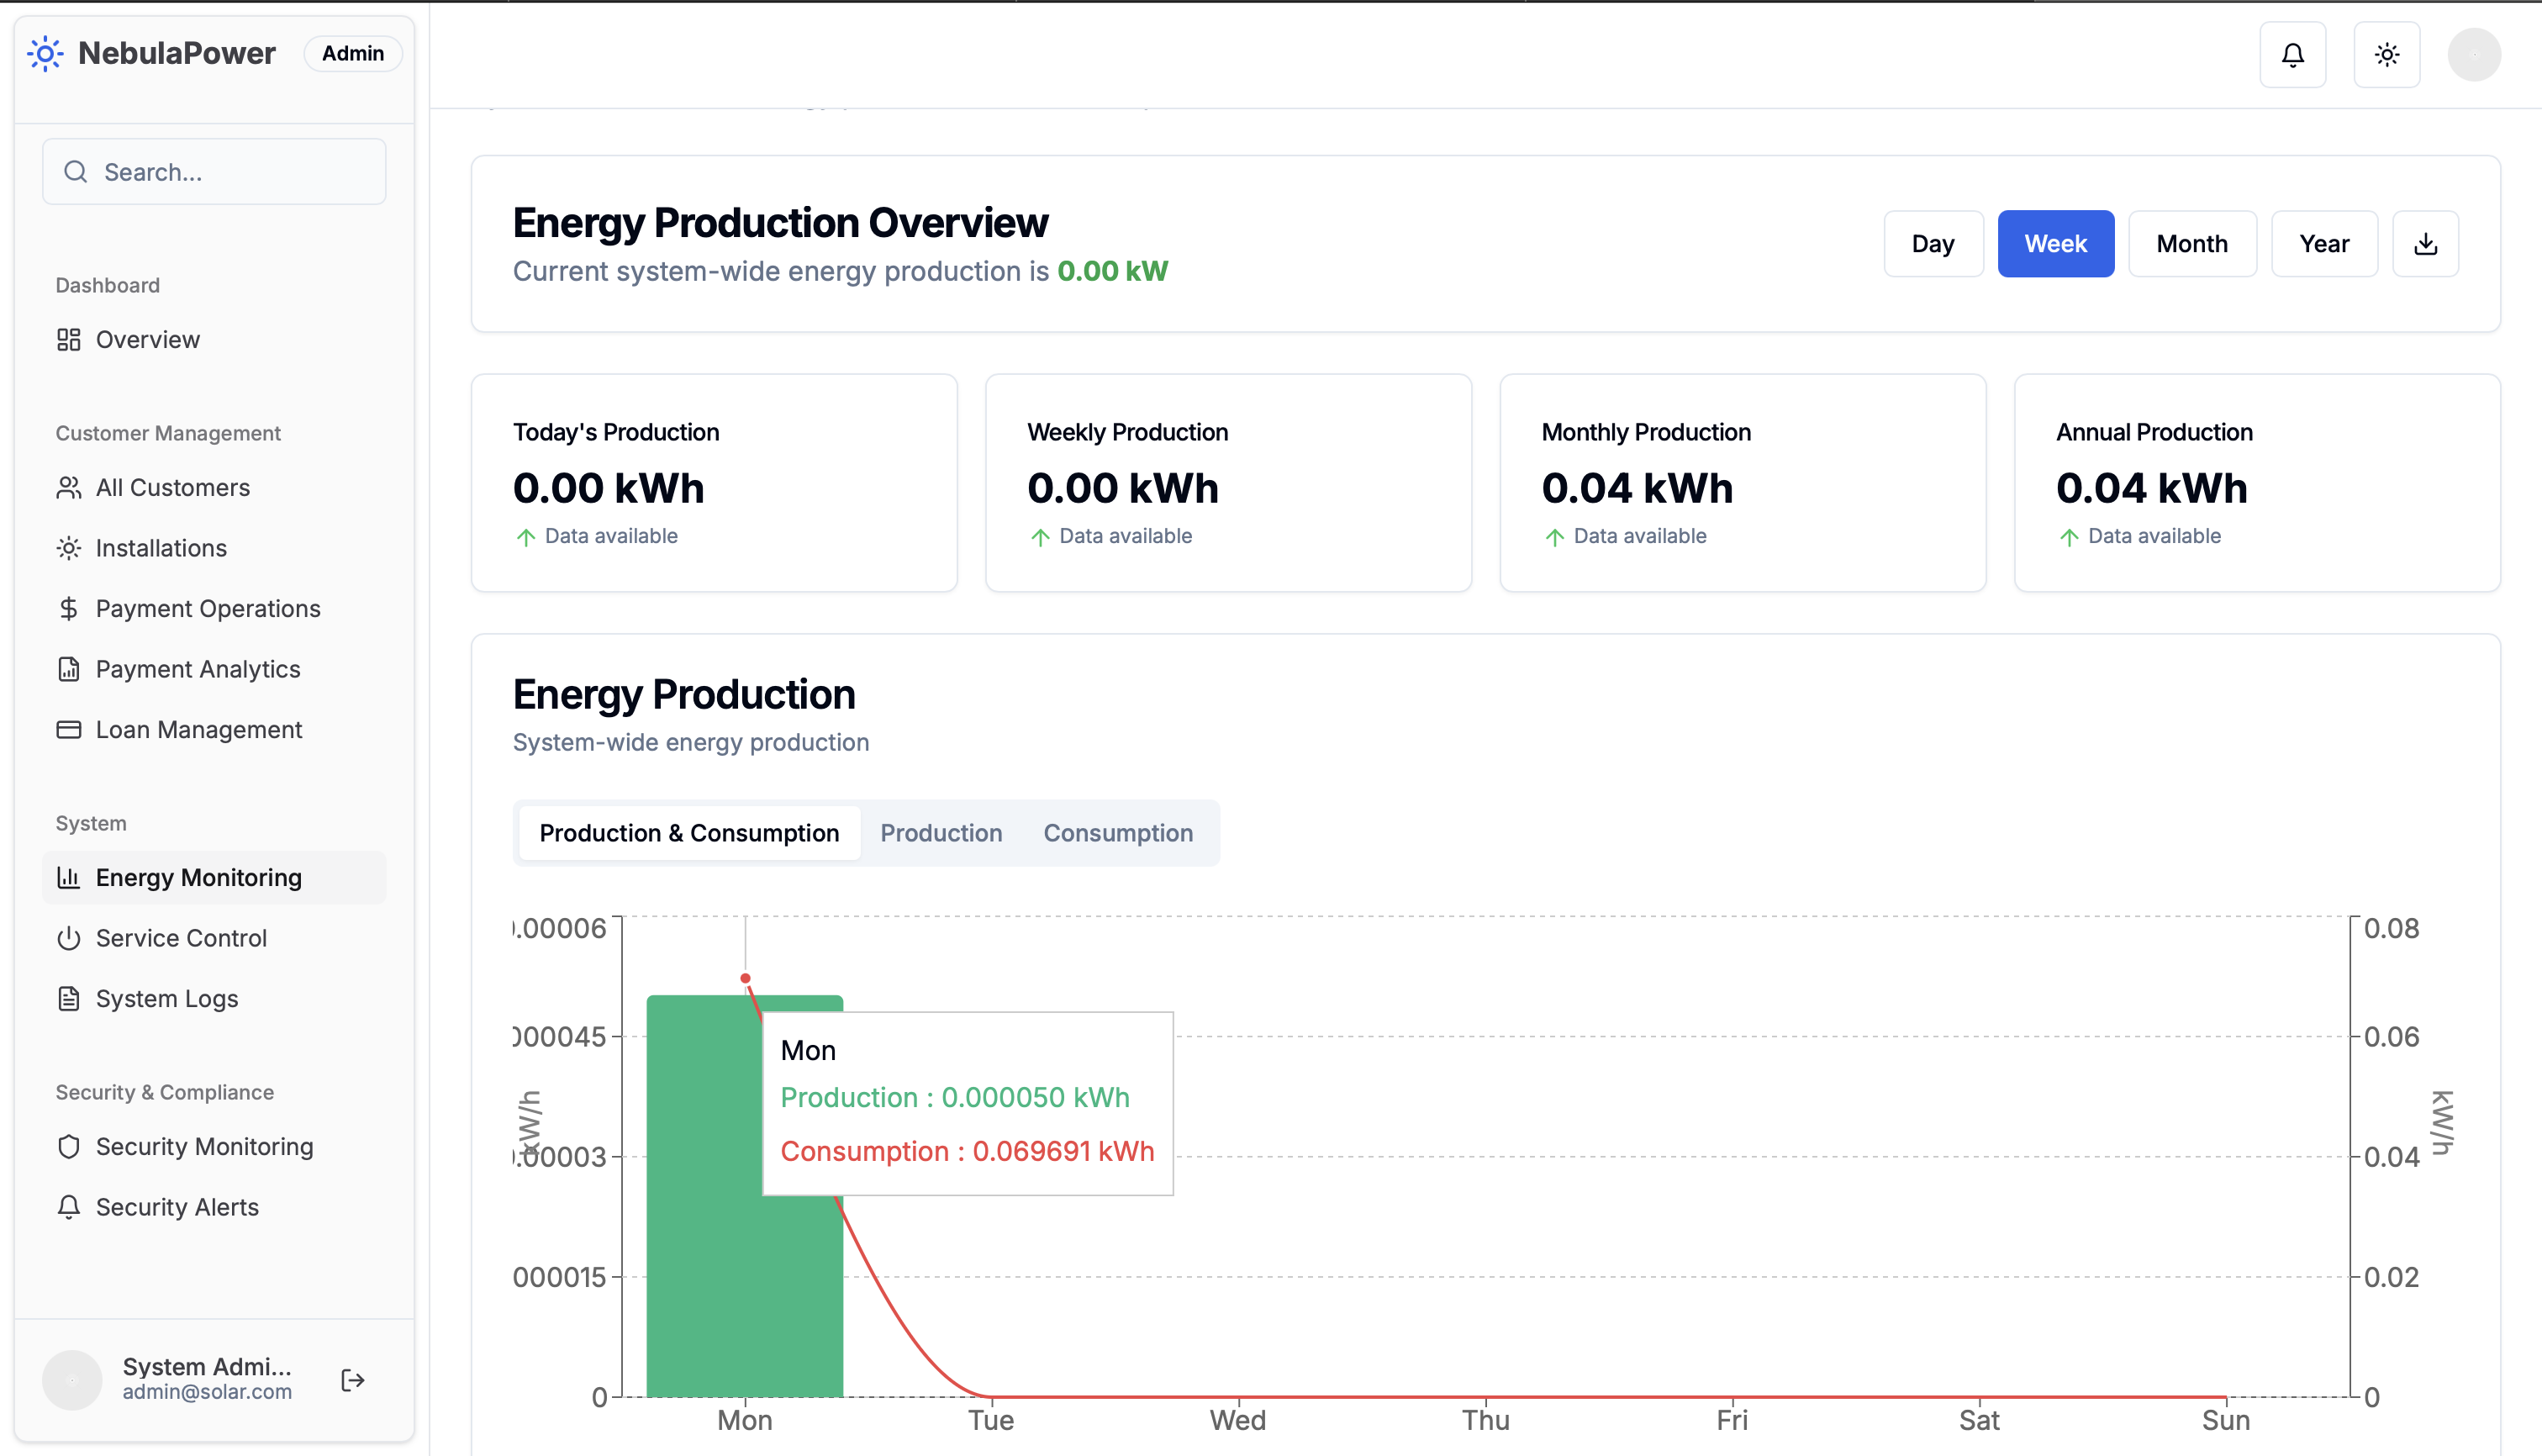
\includegraphics[width=0.85\textwidth]{images_2/admin_energy_dashb.png}
    \caption{Administrator energy monitoring}
    \label{fig:admin-energy}
\end{figure}

\subsection{Payment Operations Interface}
\label{subsec:payment-interface}

\textbf{Admin Views:} Payment analytics (trends, status tracking, Figure~\ref{fig:payment-analytics}), loan management (configuration, assignments, Figure~\ref{fig:payment-plans}), payment history (transactions, reconciliation, Figure~\ref{fig:payment-history}).

\begin{figure}[h]
    \centering
    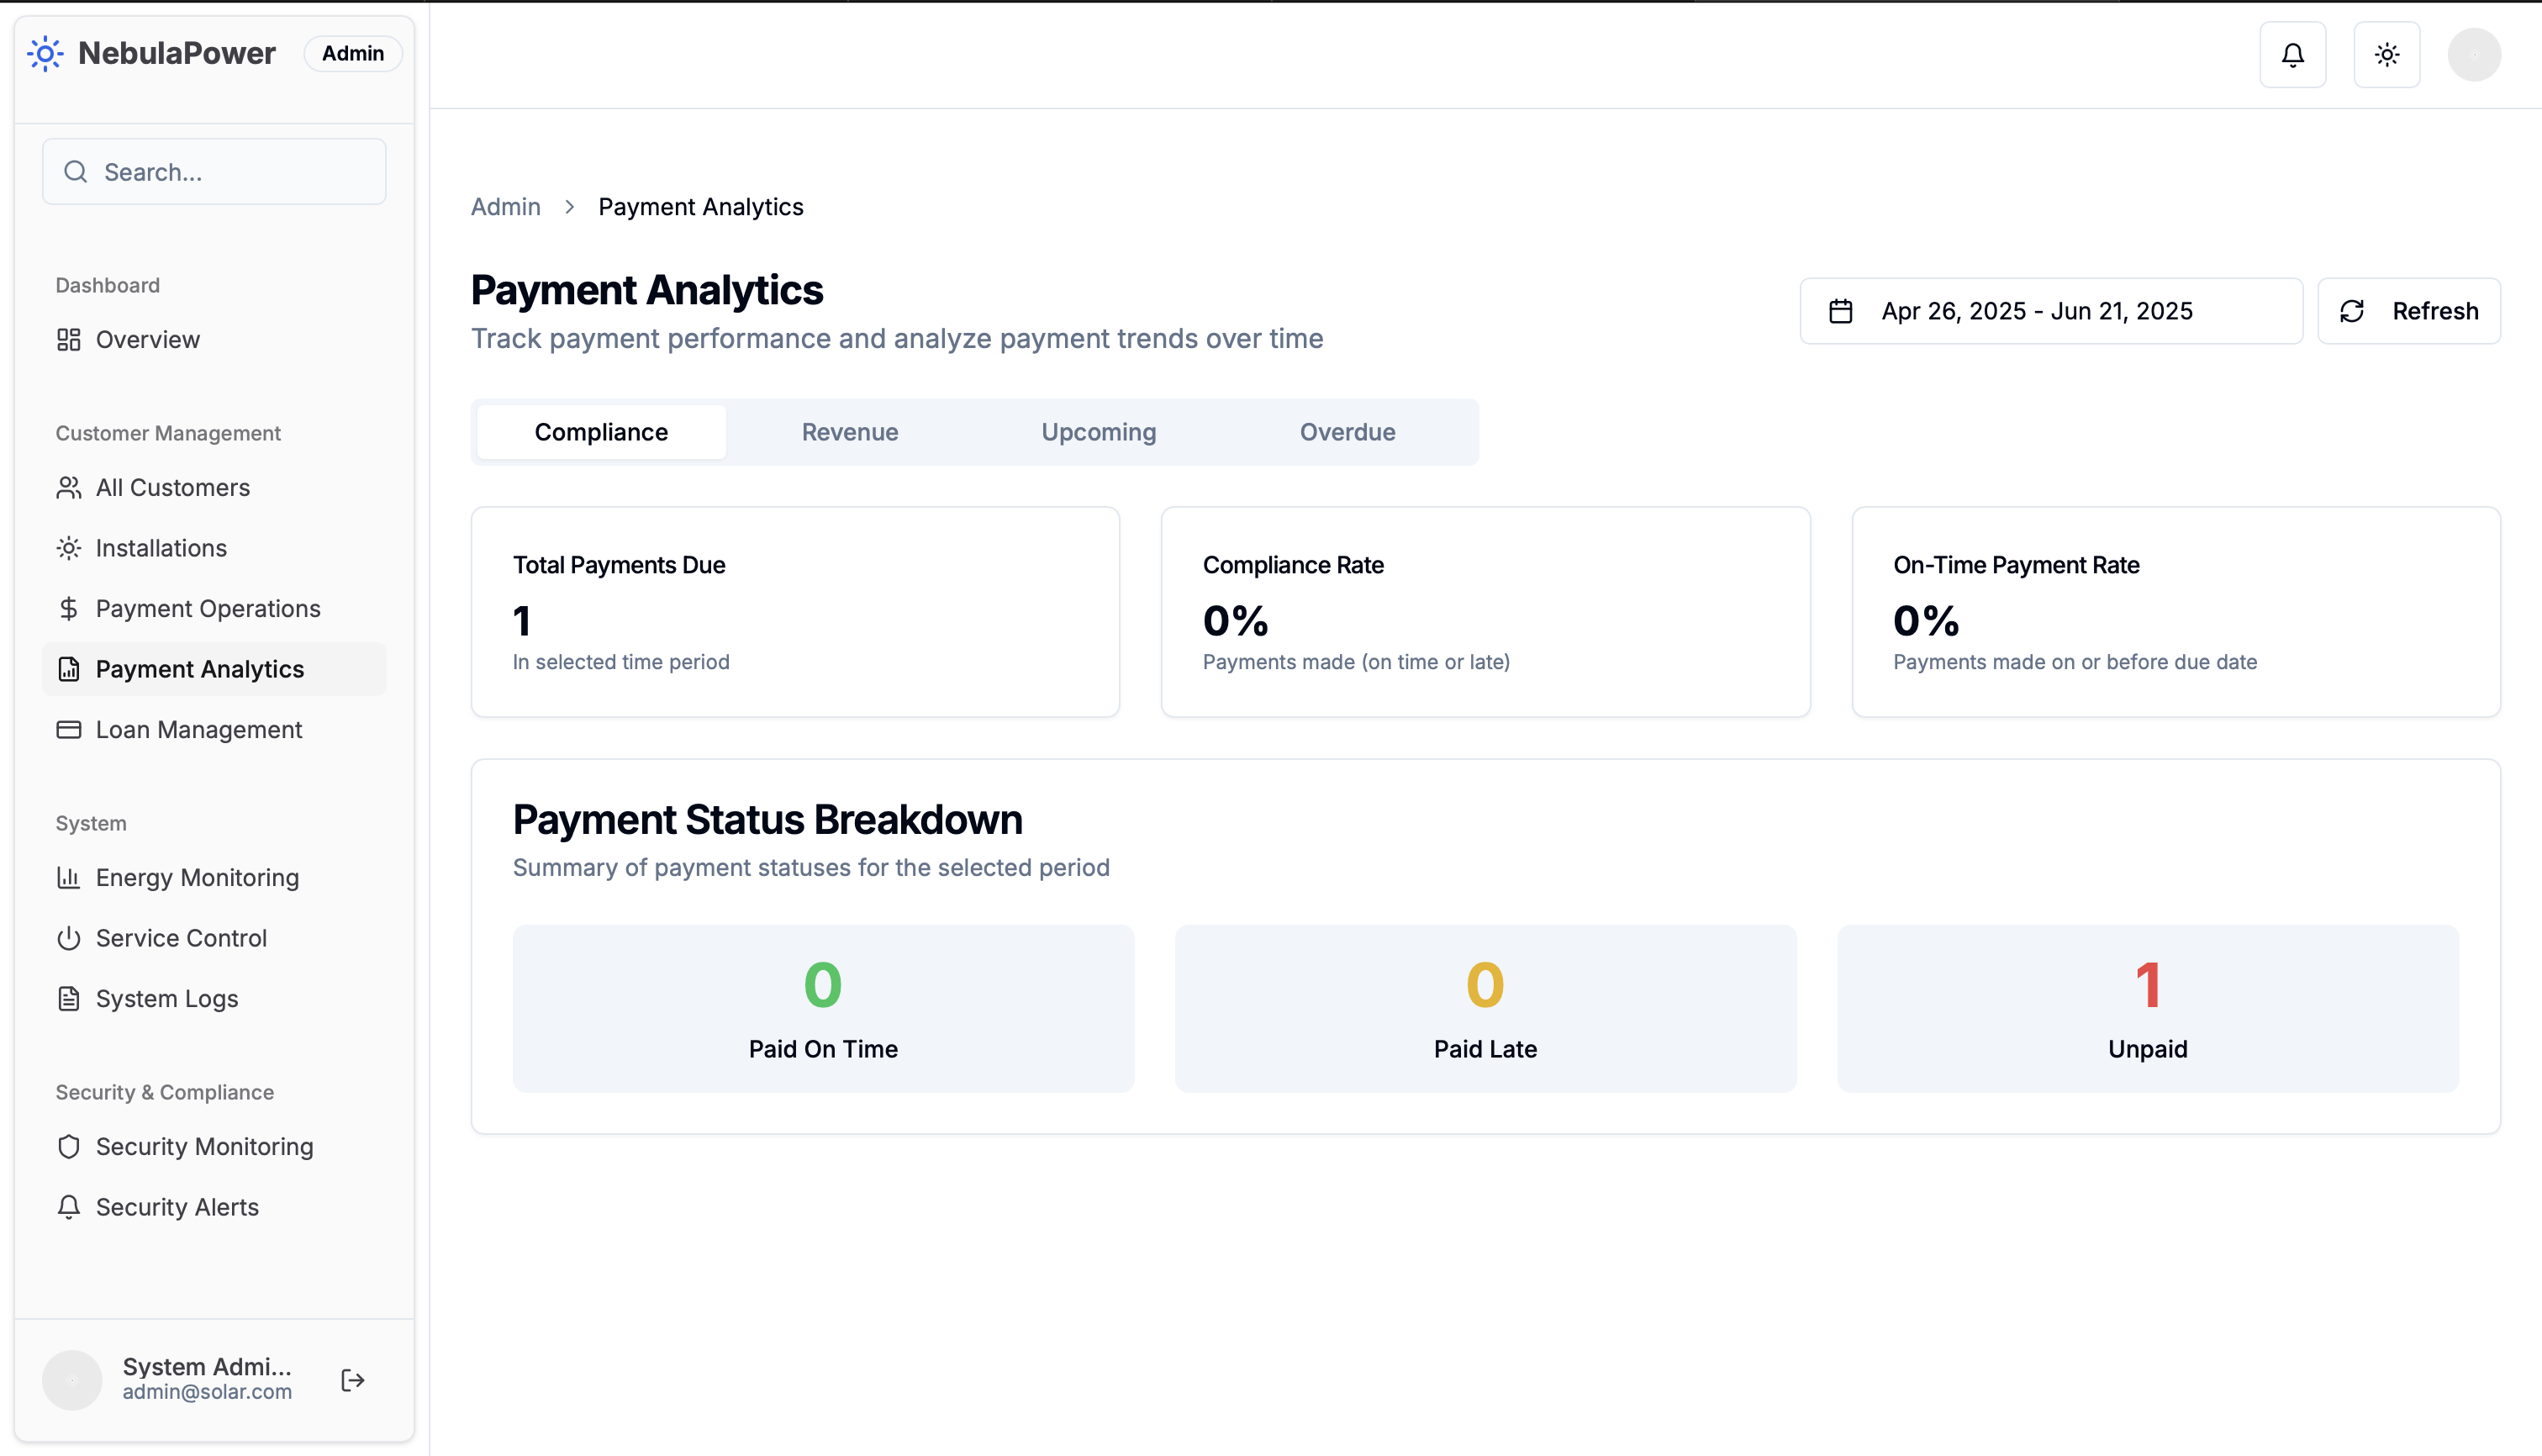
\includegraphics[width=0.85\textwidth]{images_2/payment_analytics.png}
    \caption{Payment analytics}
    \label{fig:payment-analytics}
\end{figure}

\begin{figure}[h]
    \centering
    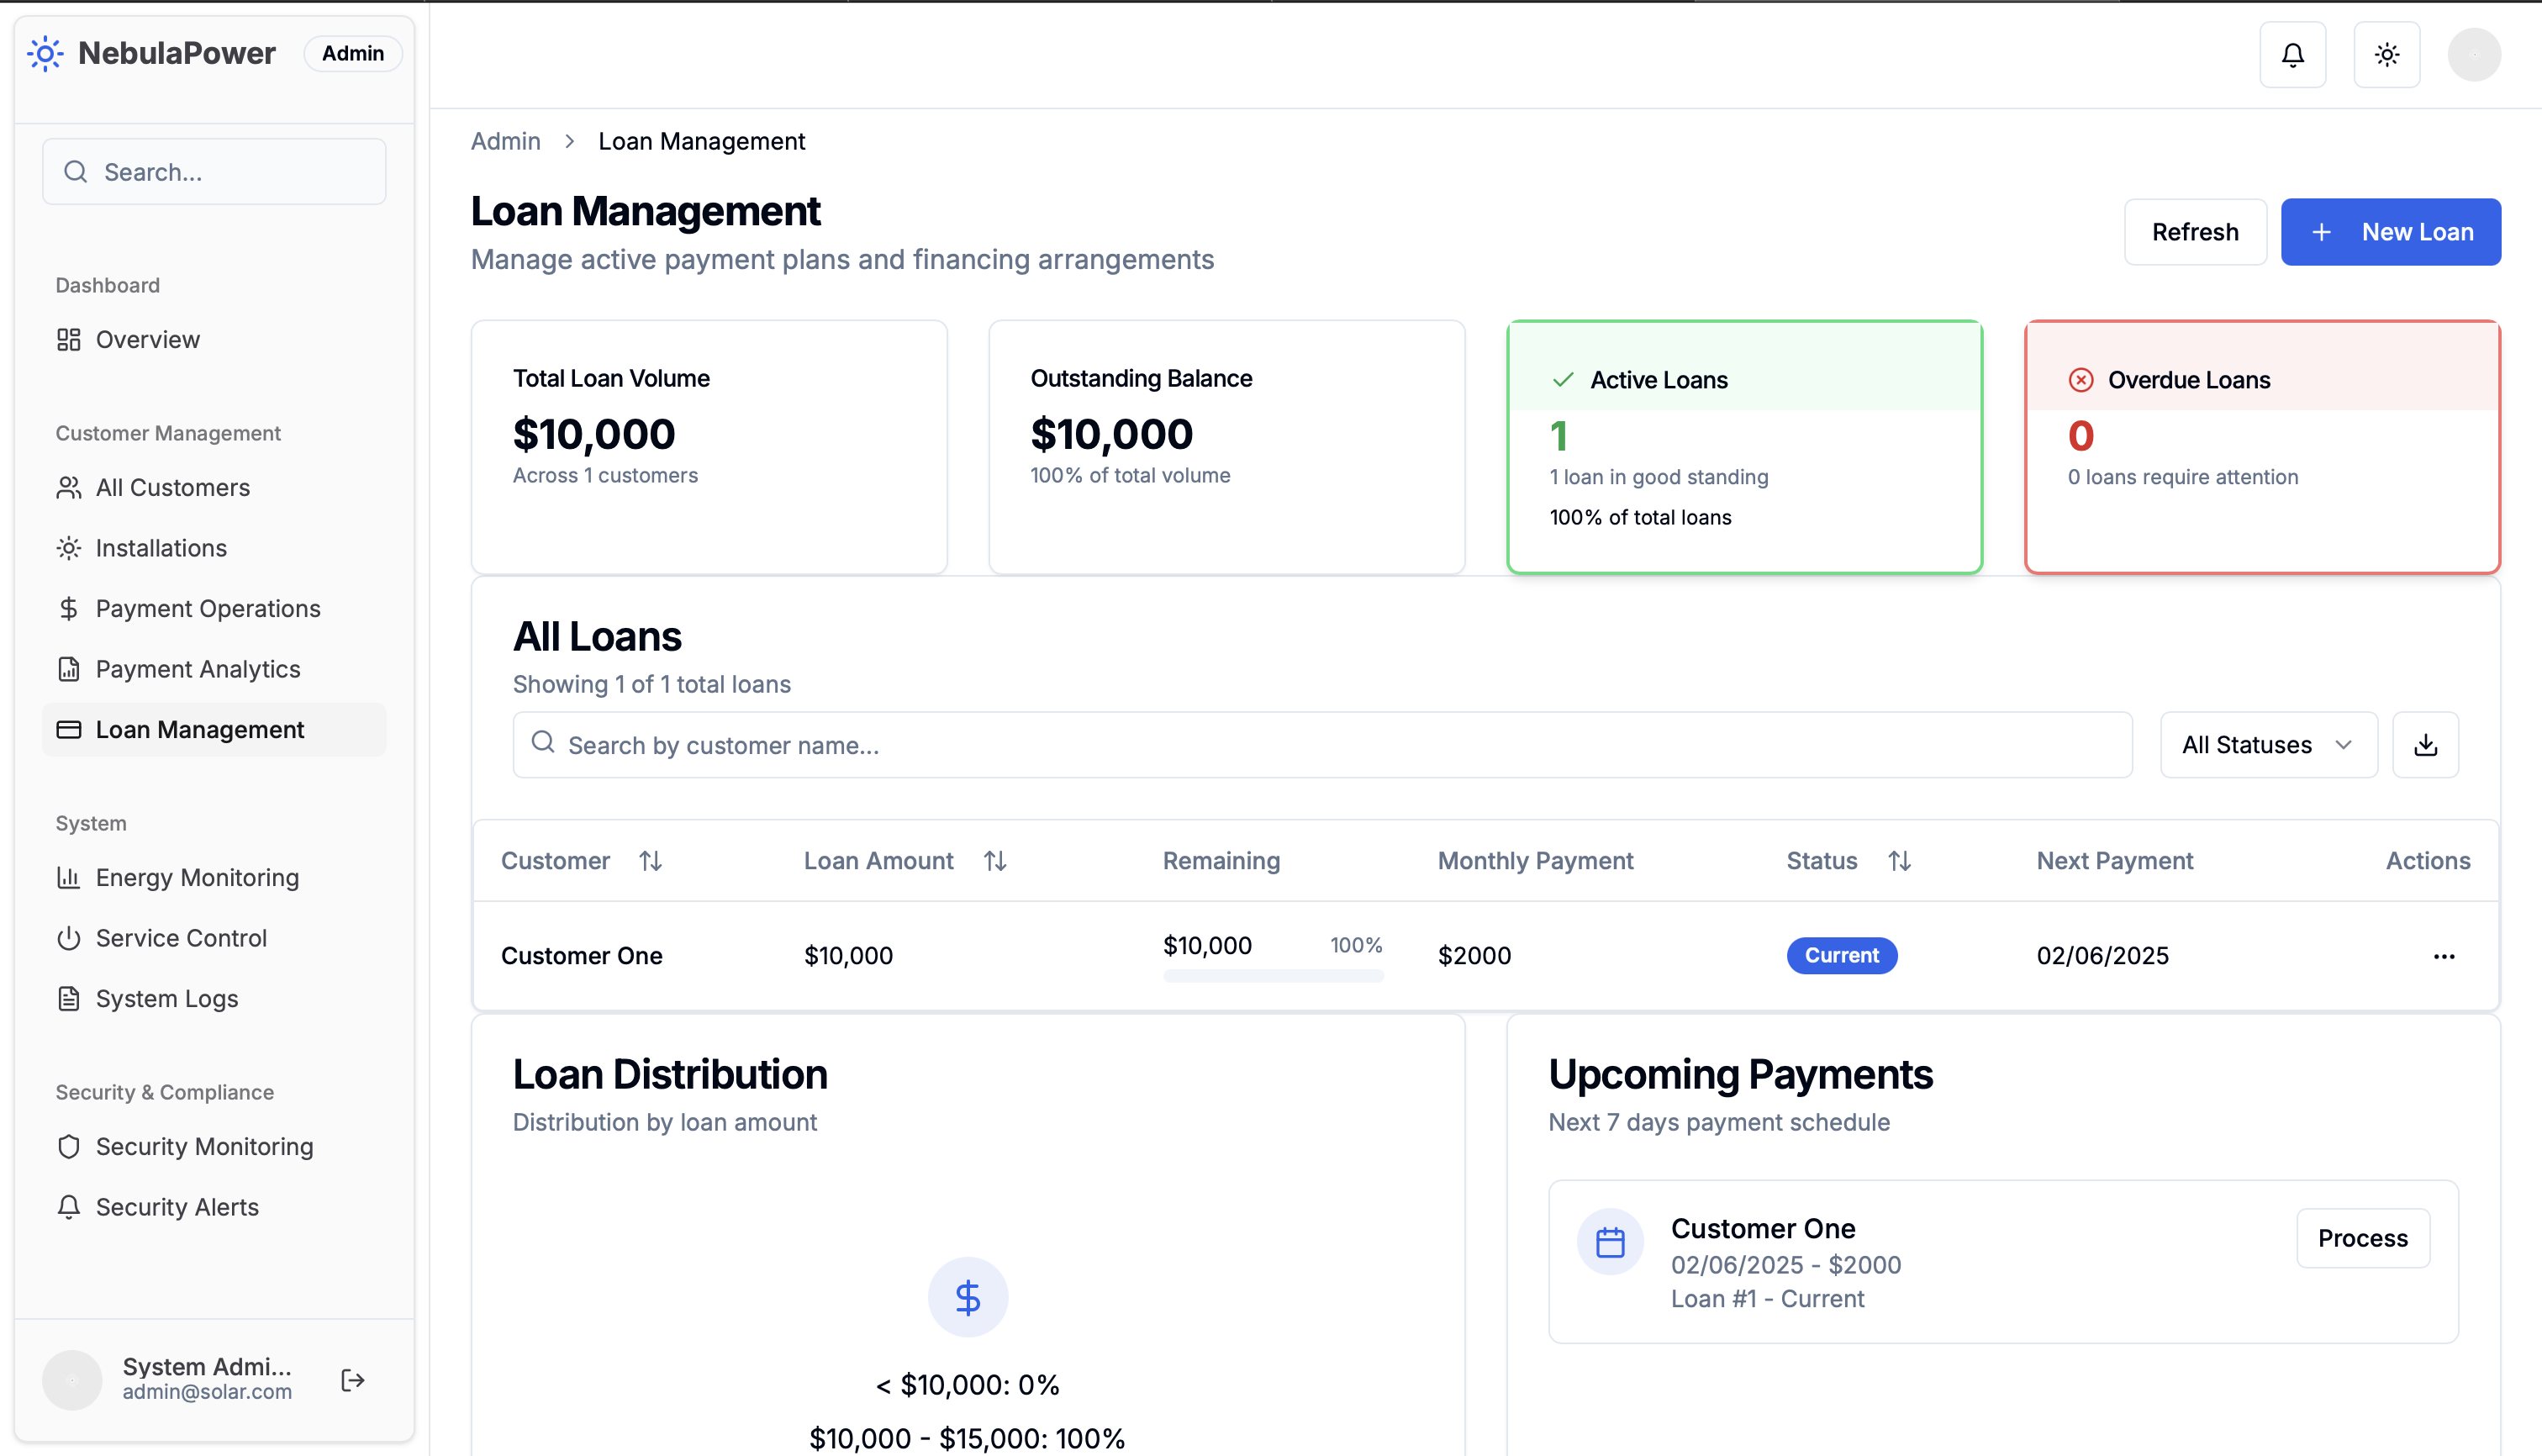
\includegraphics[width=0.85\textwidth]{images_2/loan_management.png}
    \caption{Loan management}
    \label{fig:payment-plans}
\end{figure}

\begin{figure}[h]
    \centering
    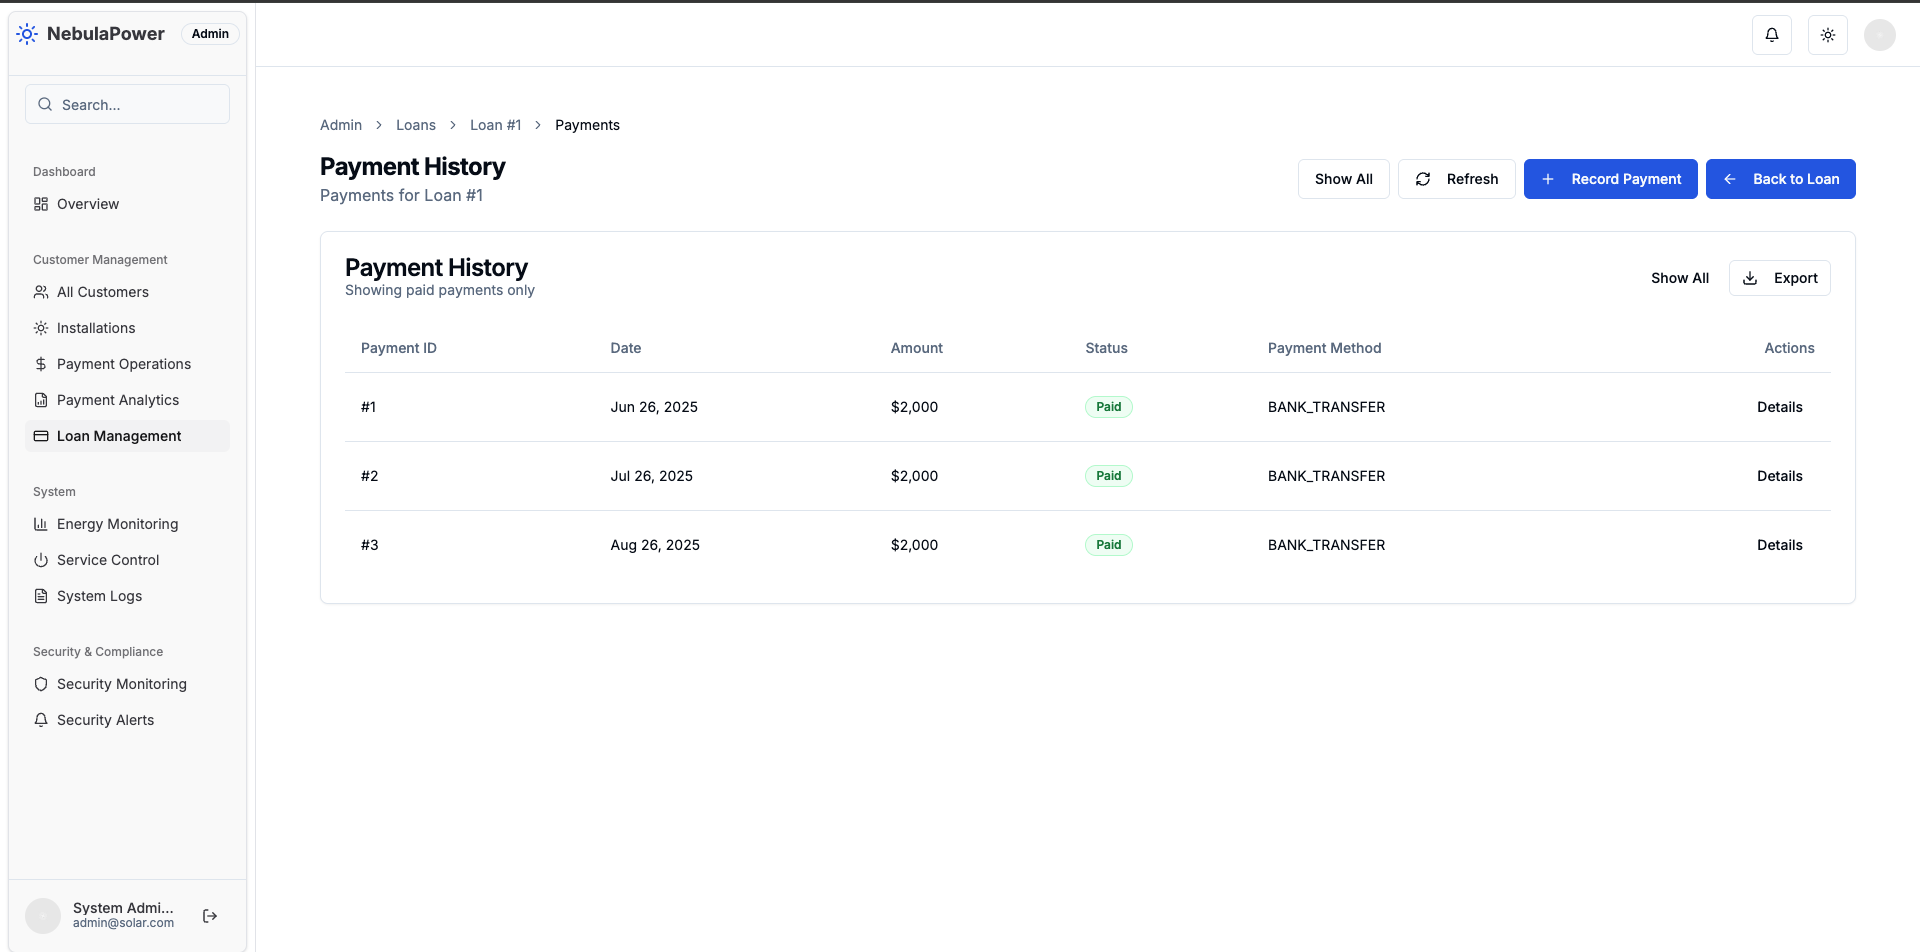
\includegraphics[width=0.85\textwidth]{images_2/admin_payment_history.png}
    \caption{Payment history}
    \label{fig:payment-history}
\end{figure}

\textbf{Customer View:} Loan summary, payment schedule, progress tracking, transaction history (Figure~\ref{fig:customer-payment-view}).

\begin{figure}[h]
    \centering
    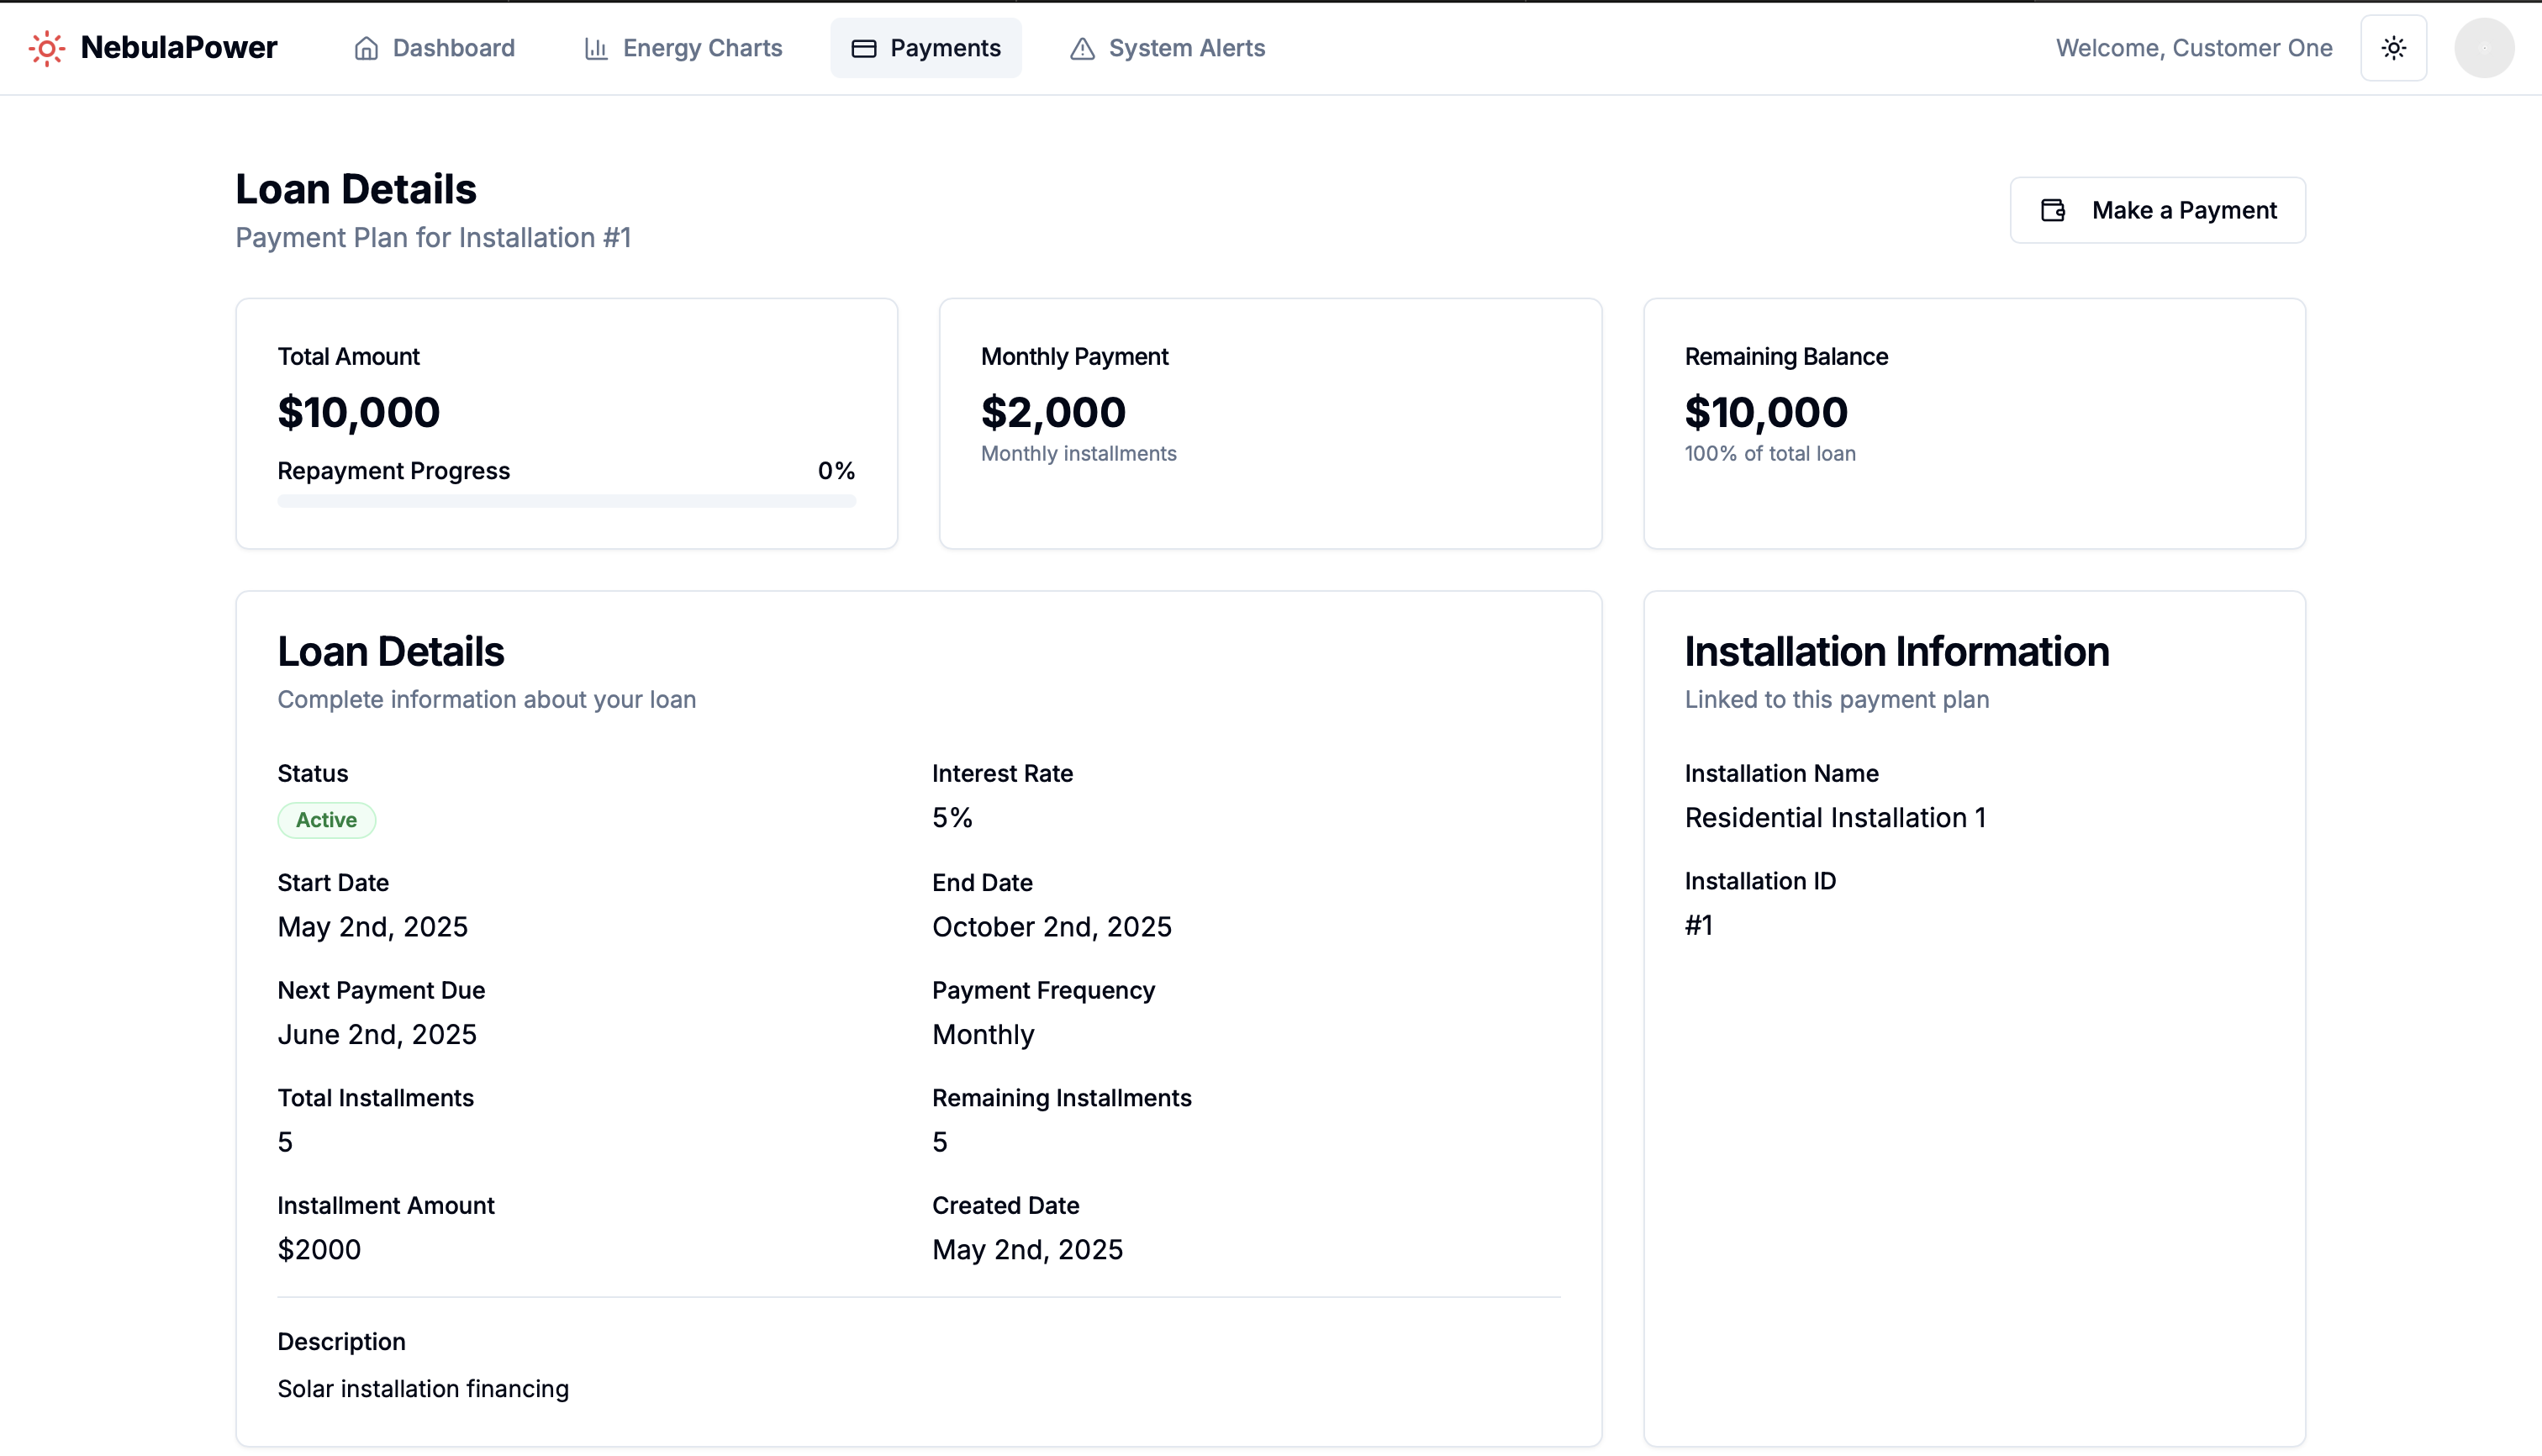
\includegraphics[width=0.85\textwidth]{images_2/customer_payments_view.png}
    \caption{Customer payment view}
    \label{fig:customer-payment-view}
\end{figure}

\subsection{Security \& Compliance Interface}
\label{subsec:security-interface}

\textbf{Security Monitoring:} Access logs, authentication status, health indicators, configuration (Figure~\ref{fig:security-monitoring}).

\begin{figure}[h]
    \centering
    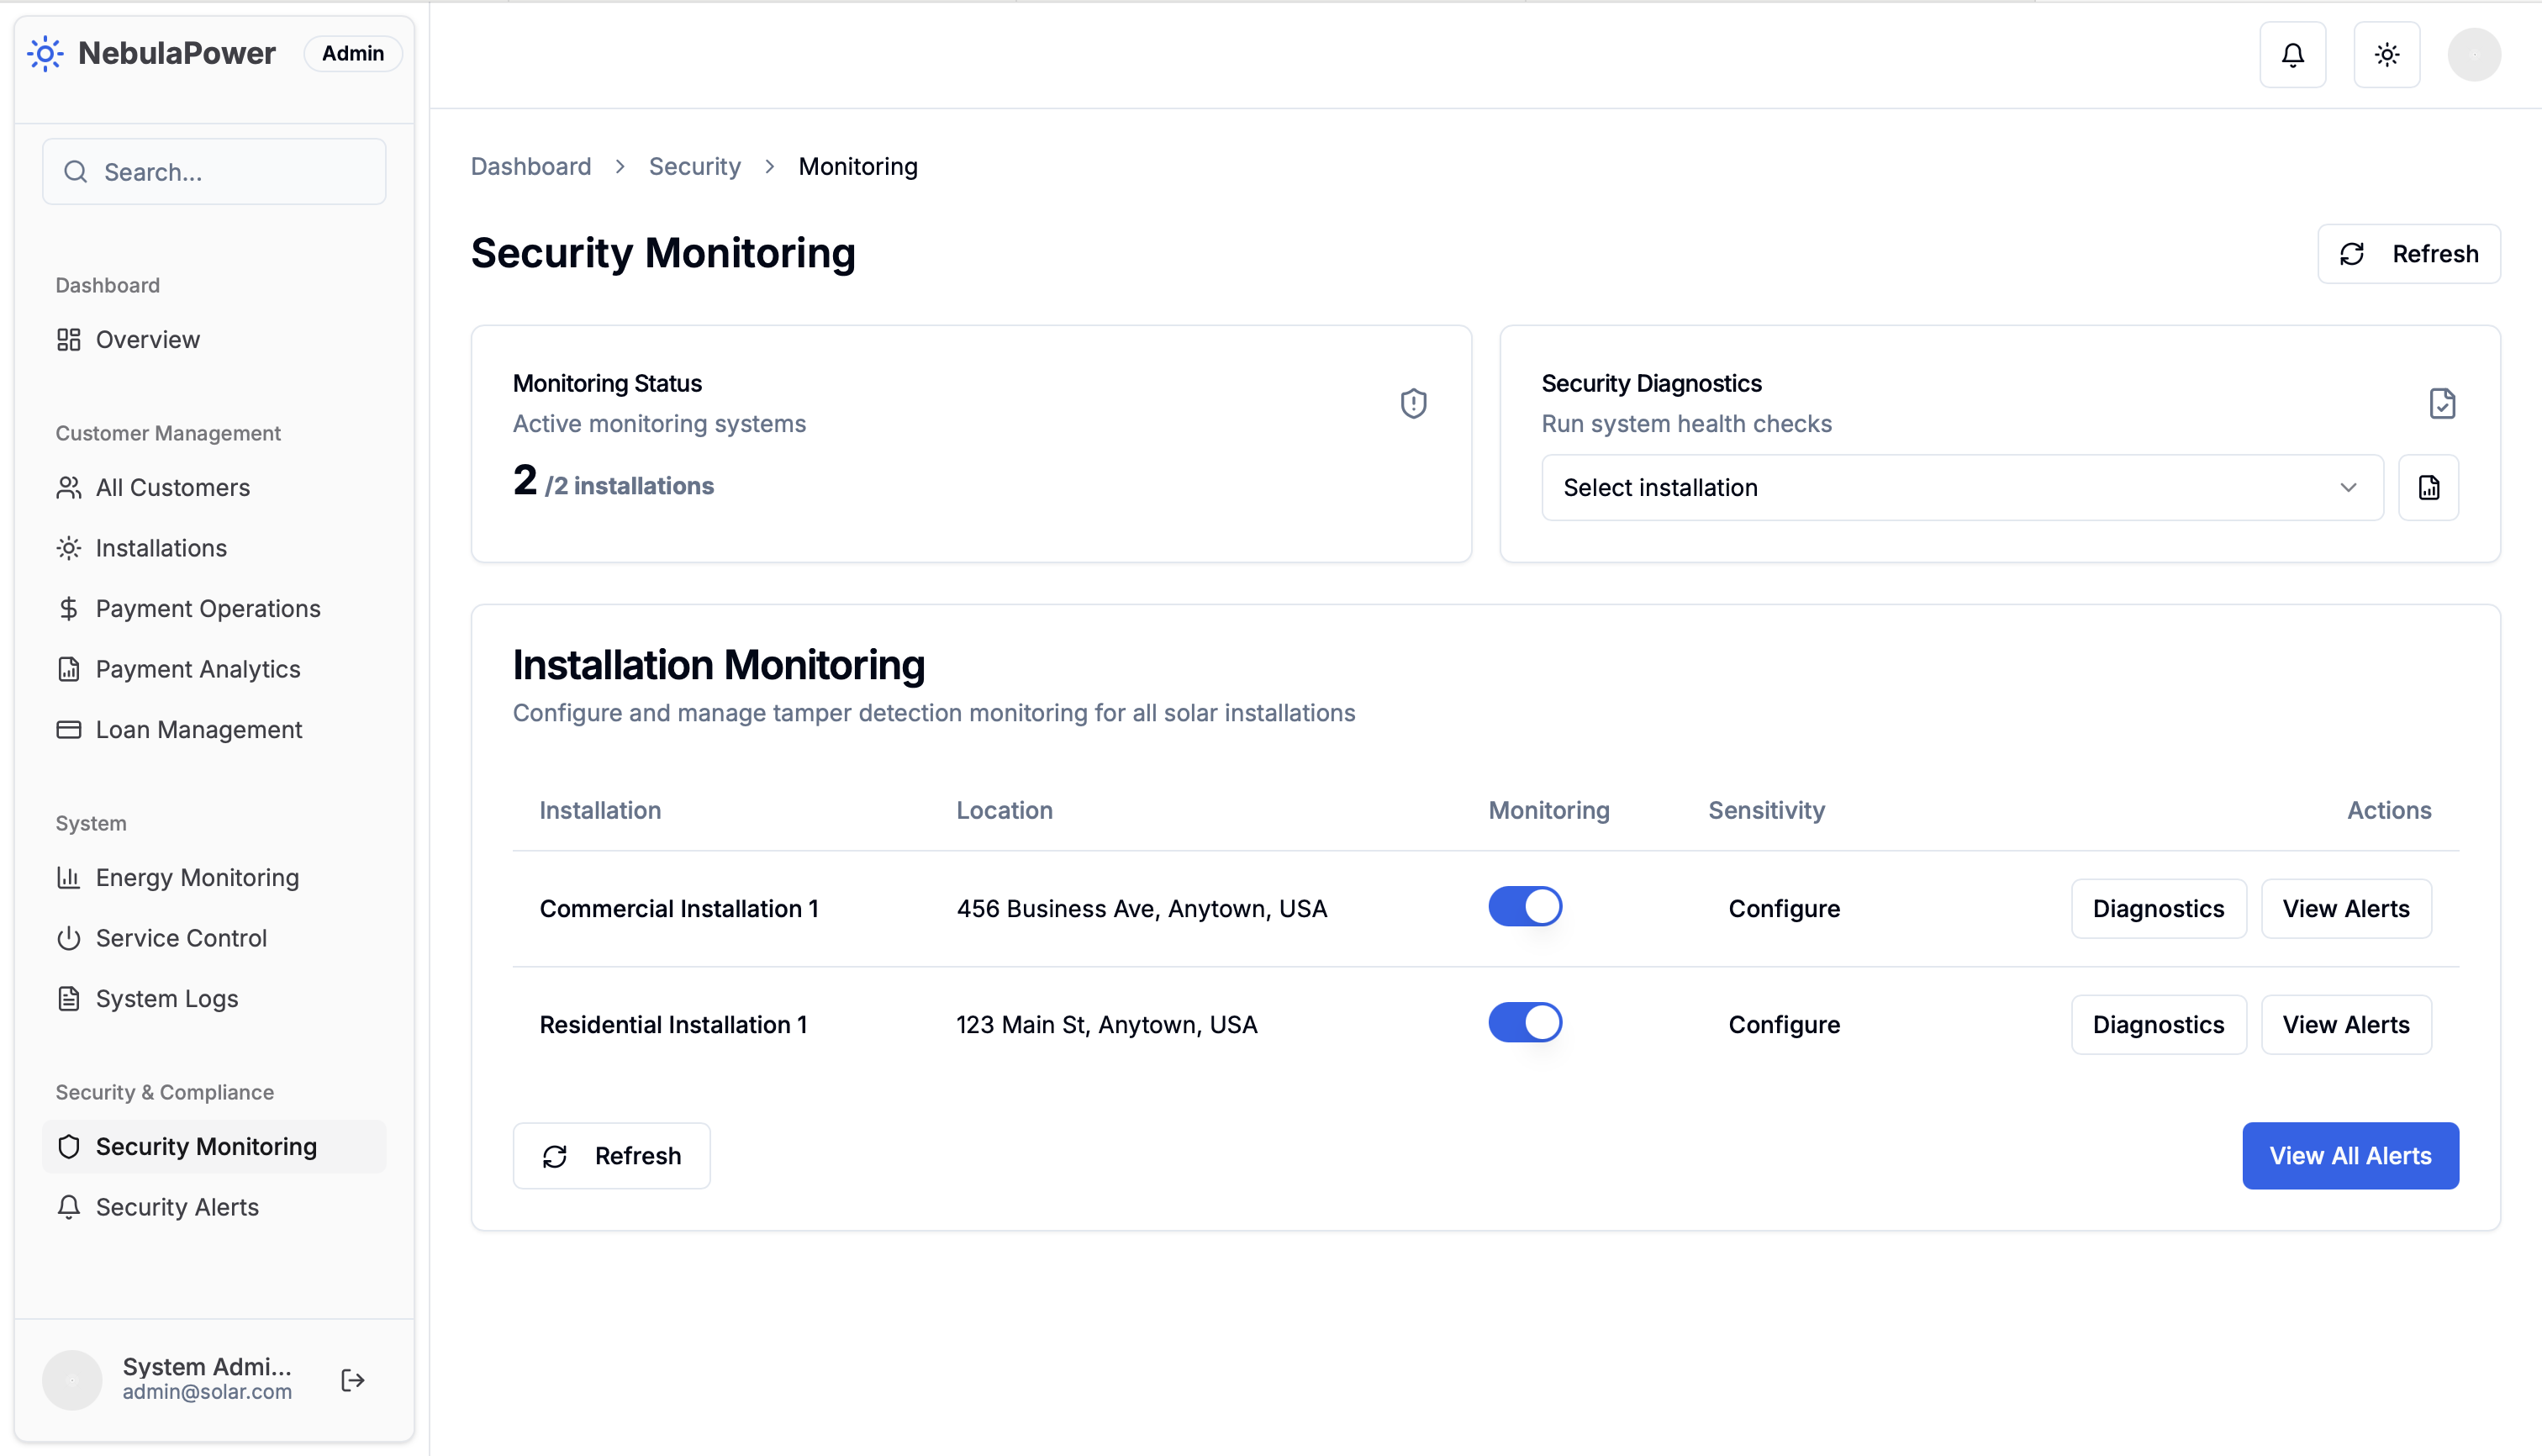
\includegraphics[width=0.85\textwidth]{images_2/admin_security_monitoring.png}
    \caption{Security monitoring}
    \label{fig:security-monitoring}
\end{figure}

\textbf{Admin Alerts:} Dashboard with alert counts, filtering (open/closed/in-progress), severity classification, response actions (Figure~\ref{fig:security-alerts-admin}).

\begin{figure}[h]
    \centering
    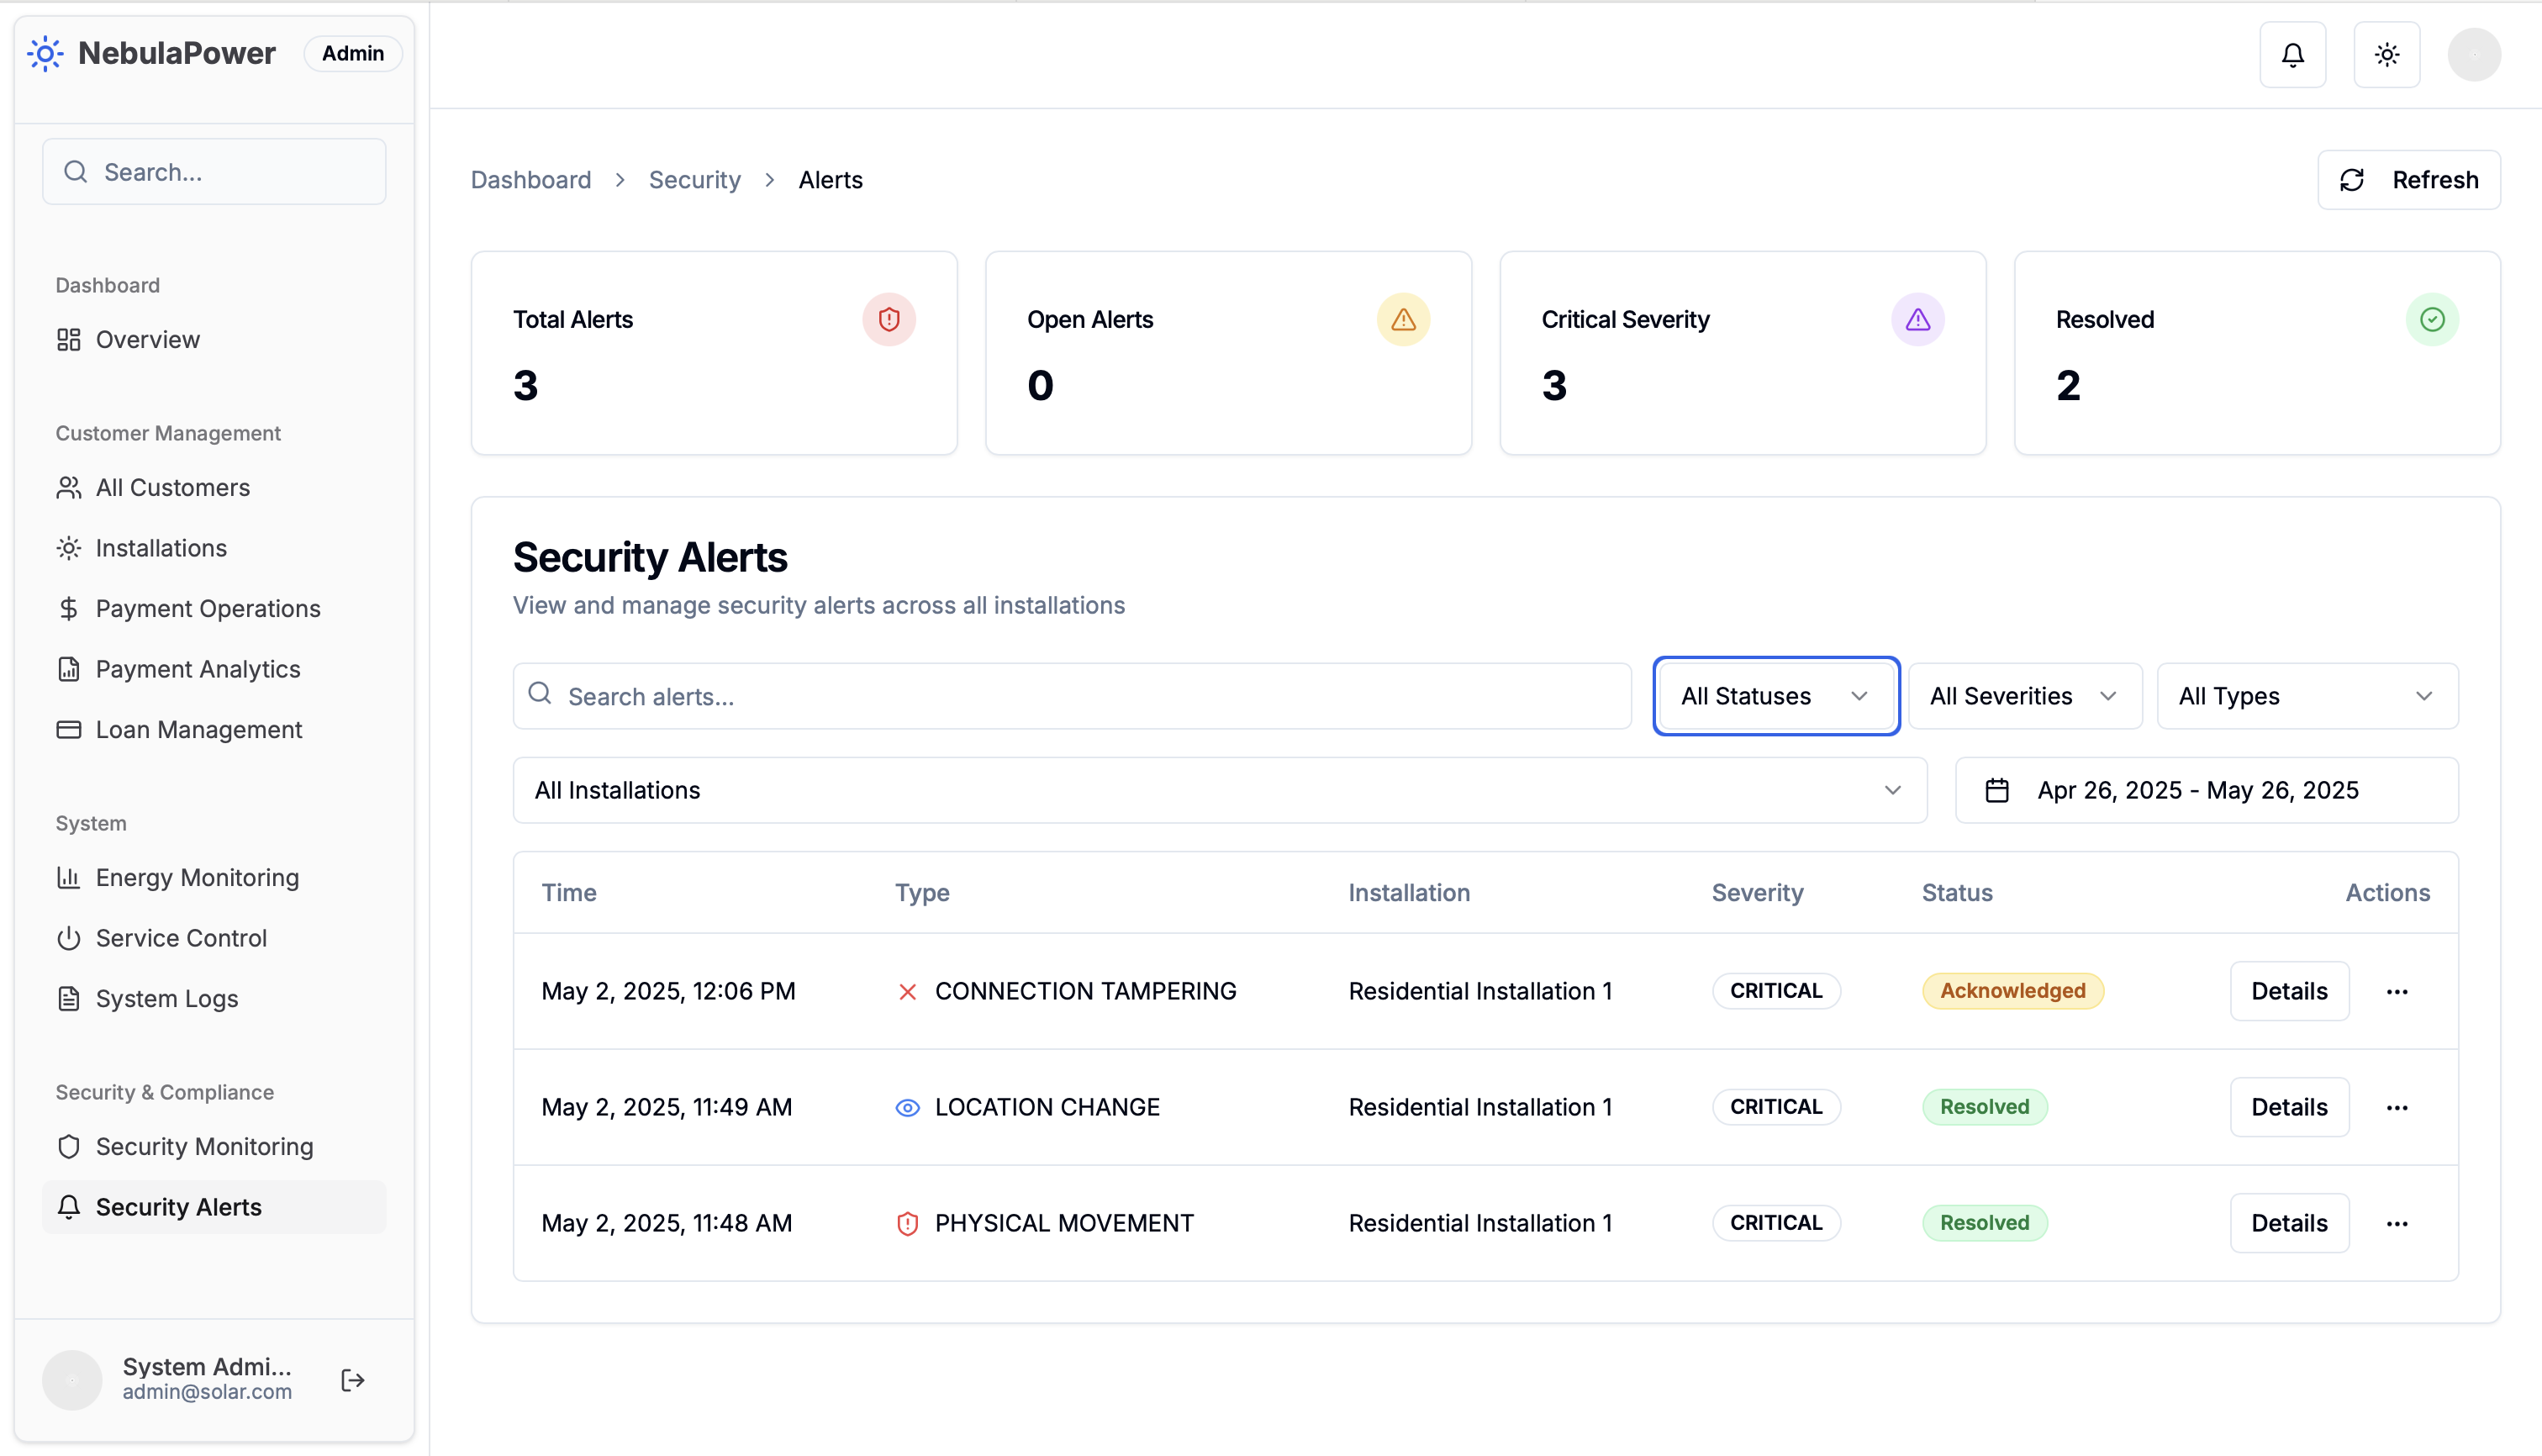
\includegraphics[width=0.85\textwidth]{images_2/admin_alerts.png}
    \caption{Admin security alerts}
    \label{fig:security-alerts-admin}
\end{figure}

\textbf{Customer Alerts:} Installation-specific alerts with status and recommended actions (Figure~\ref{fig:security-alerts-customer}).

\begin{figure}[h]
    \centering
    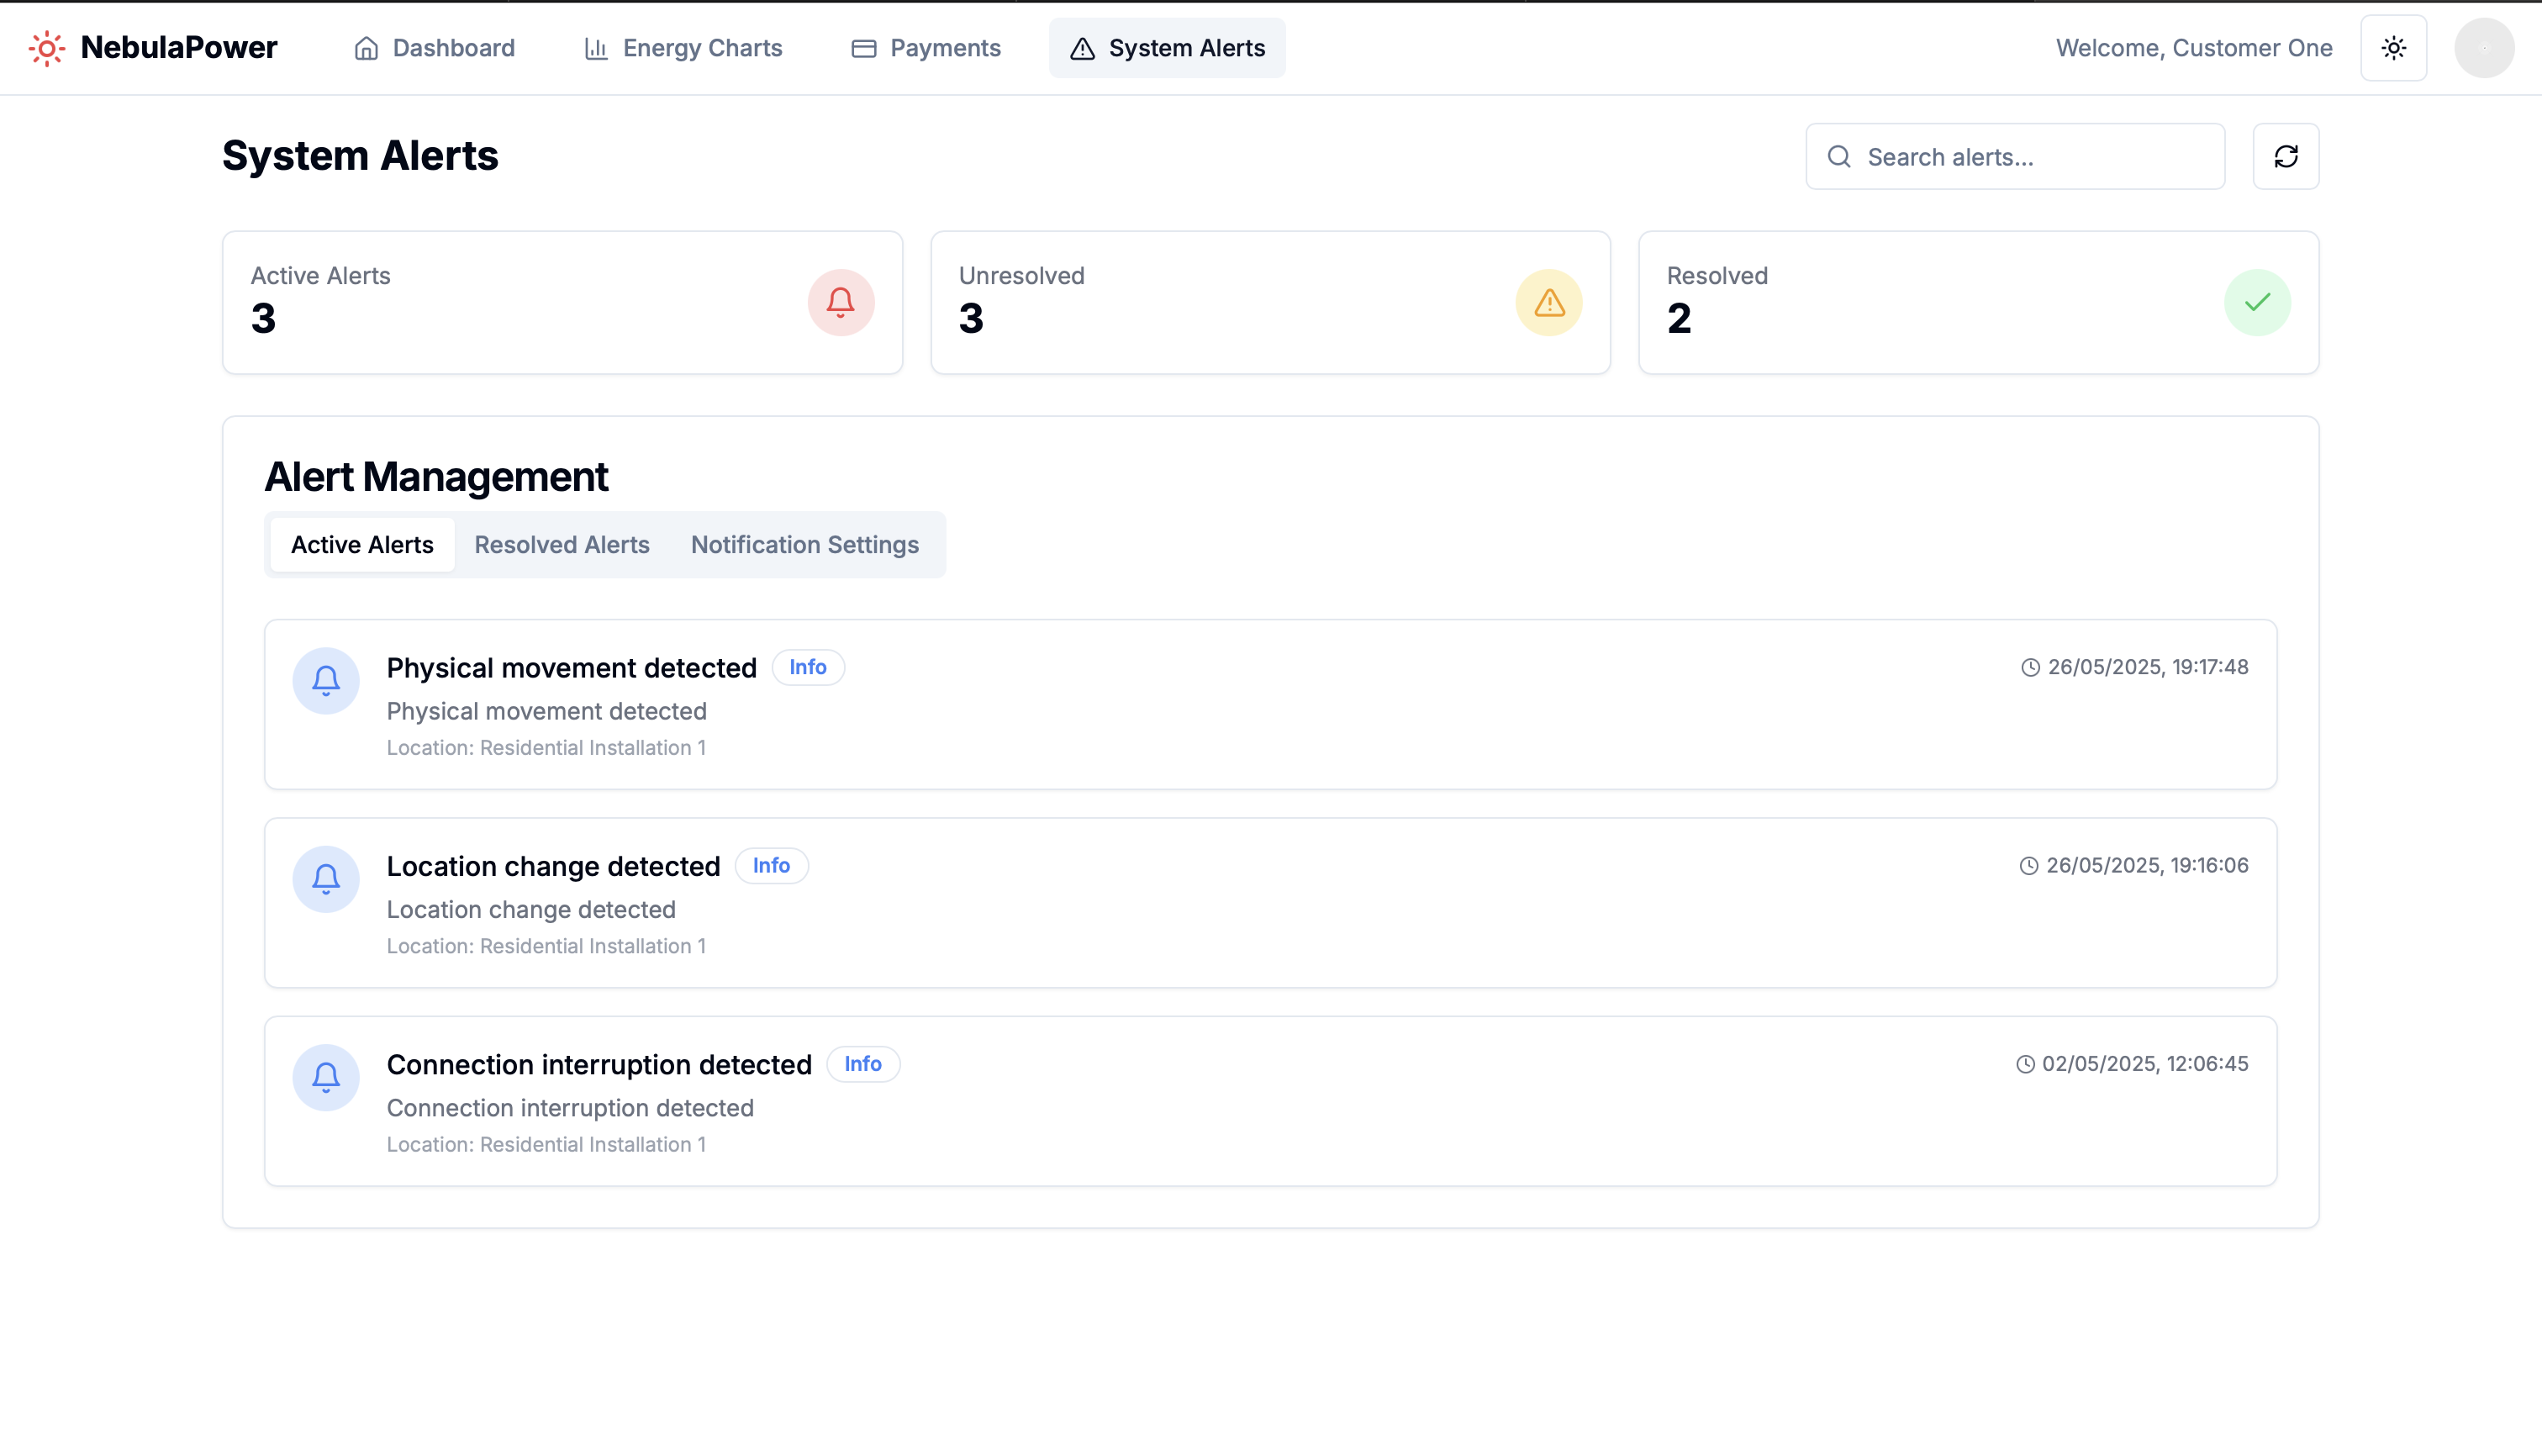
\includegraphics[width=0.85\textwidth]{images_2/customer_alert.png}
    \caption{Customer security alerts}
    \label{fig:security-alerts-customer}
\end{figure}

\subsubsection{System Logs}

\textbf{Operational Logs:} Service logs, errors/warnings, start/stop events, connection status. \textbf{Security Logs:} Audit logs, tamper detection, authentication attempts, authorization violations. Logs support filtering, search, and export (Figures~\ref{fig:system-logs}-\ref{fig:log-status}).

\begin{figure}[h]
    \centering
    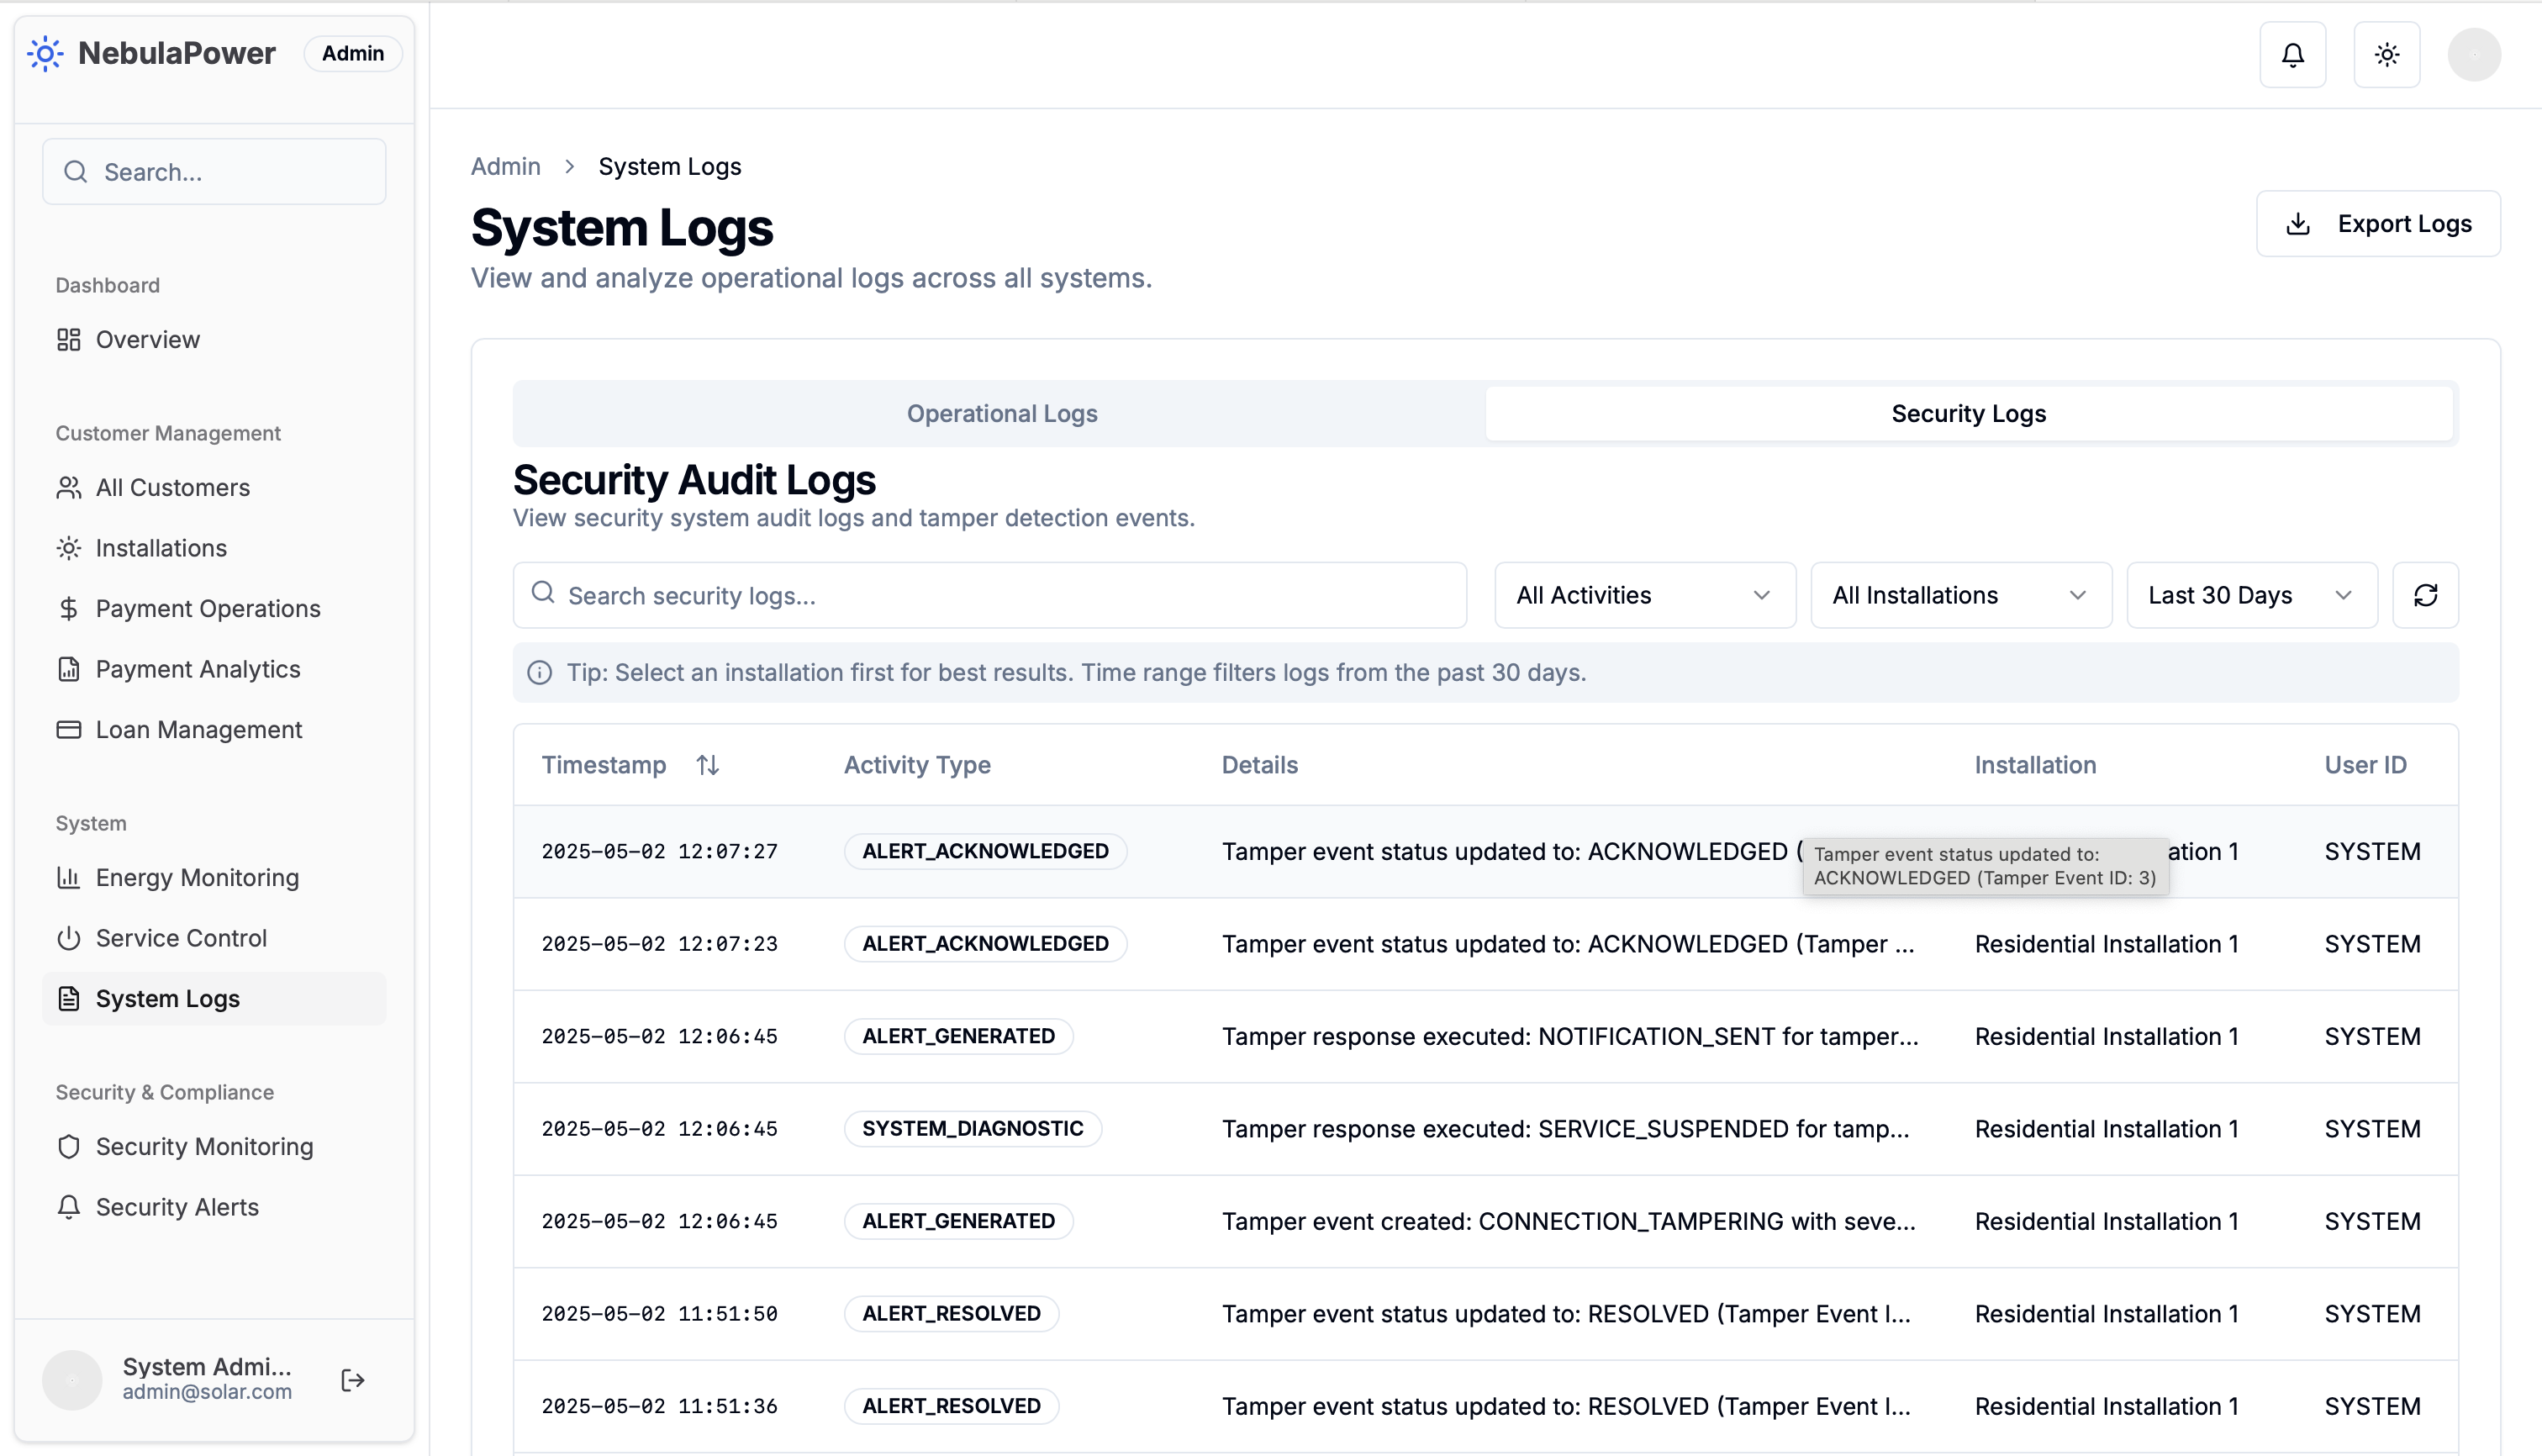
\includegraphics[width=0.8\textwidth]{images_2/admin_system_logs.png}
    \caption{System logs}
    \label{fig:system-logs}
\end{figure}

\begin{figure}[h]
    \centering
    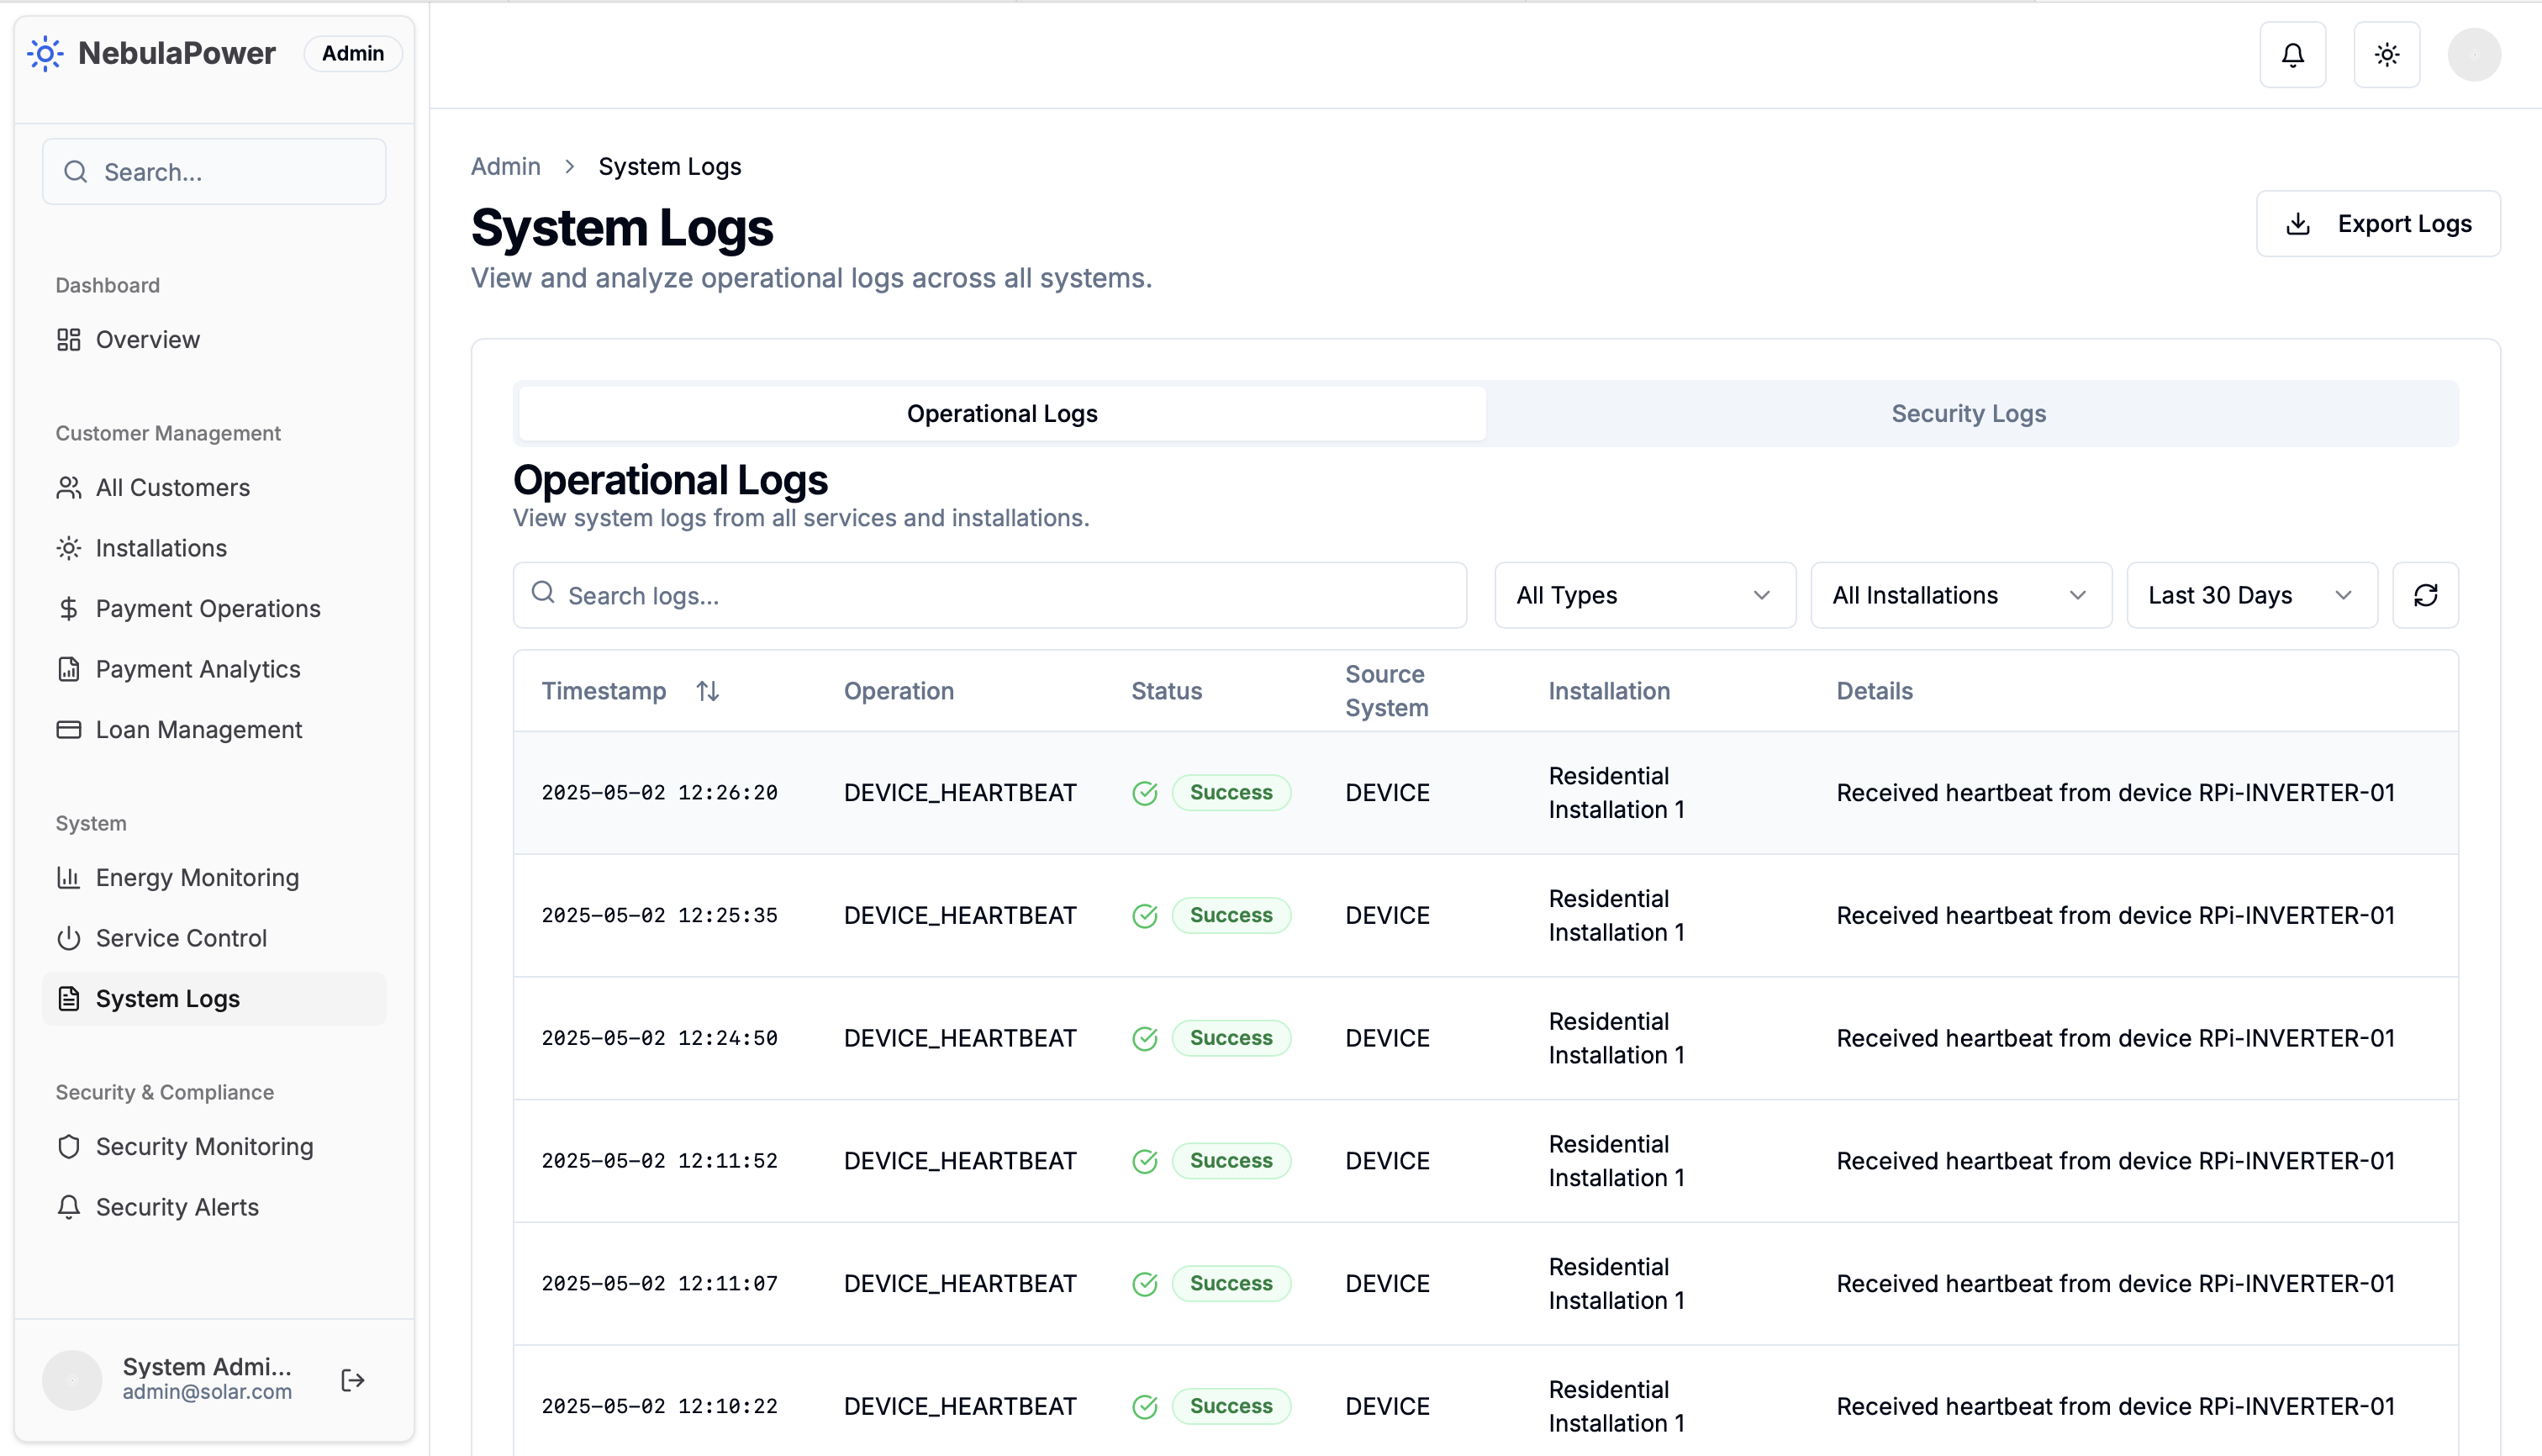
\includegraphics[width=0.8\textwidth]{images_2/admin_op_logs.png}
    \caption{Operational logs}
    \label{fig:operational-logs}
\end{figure}

\begin{figure}[h]
    \centering
    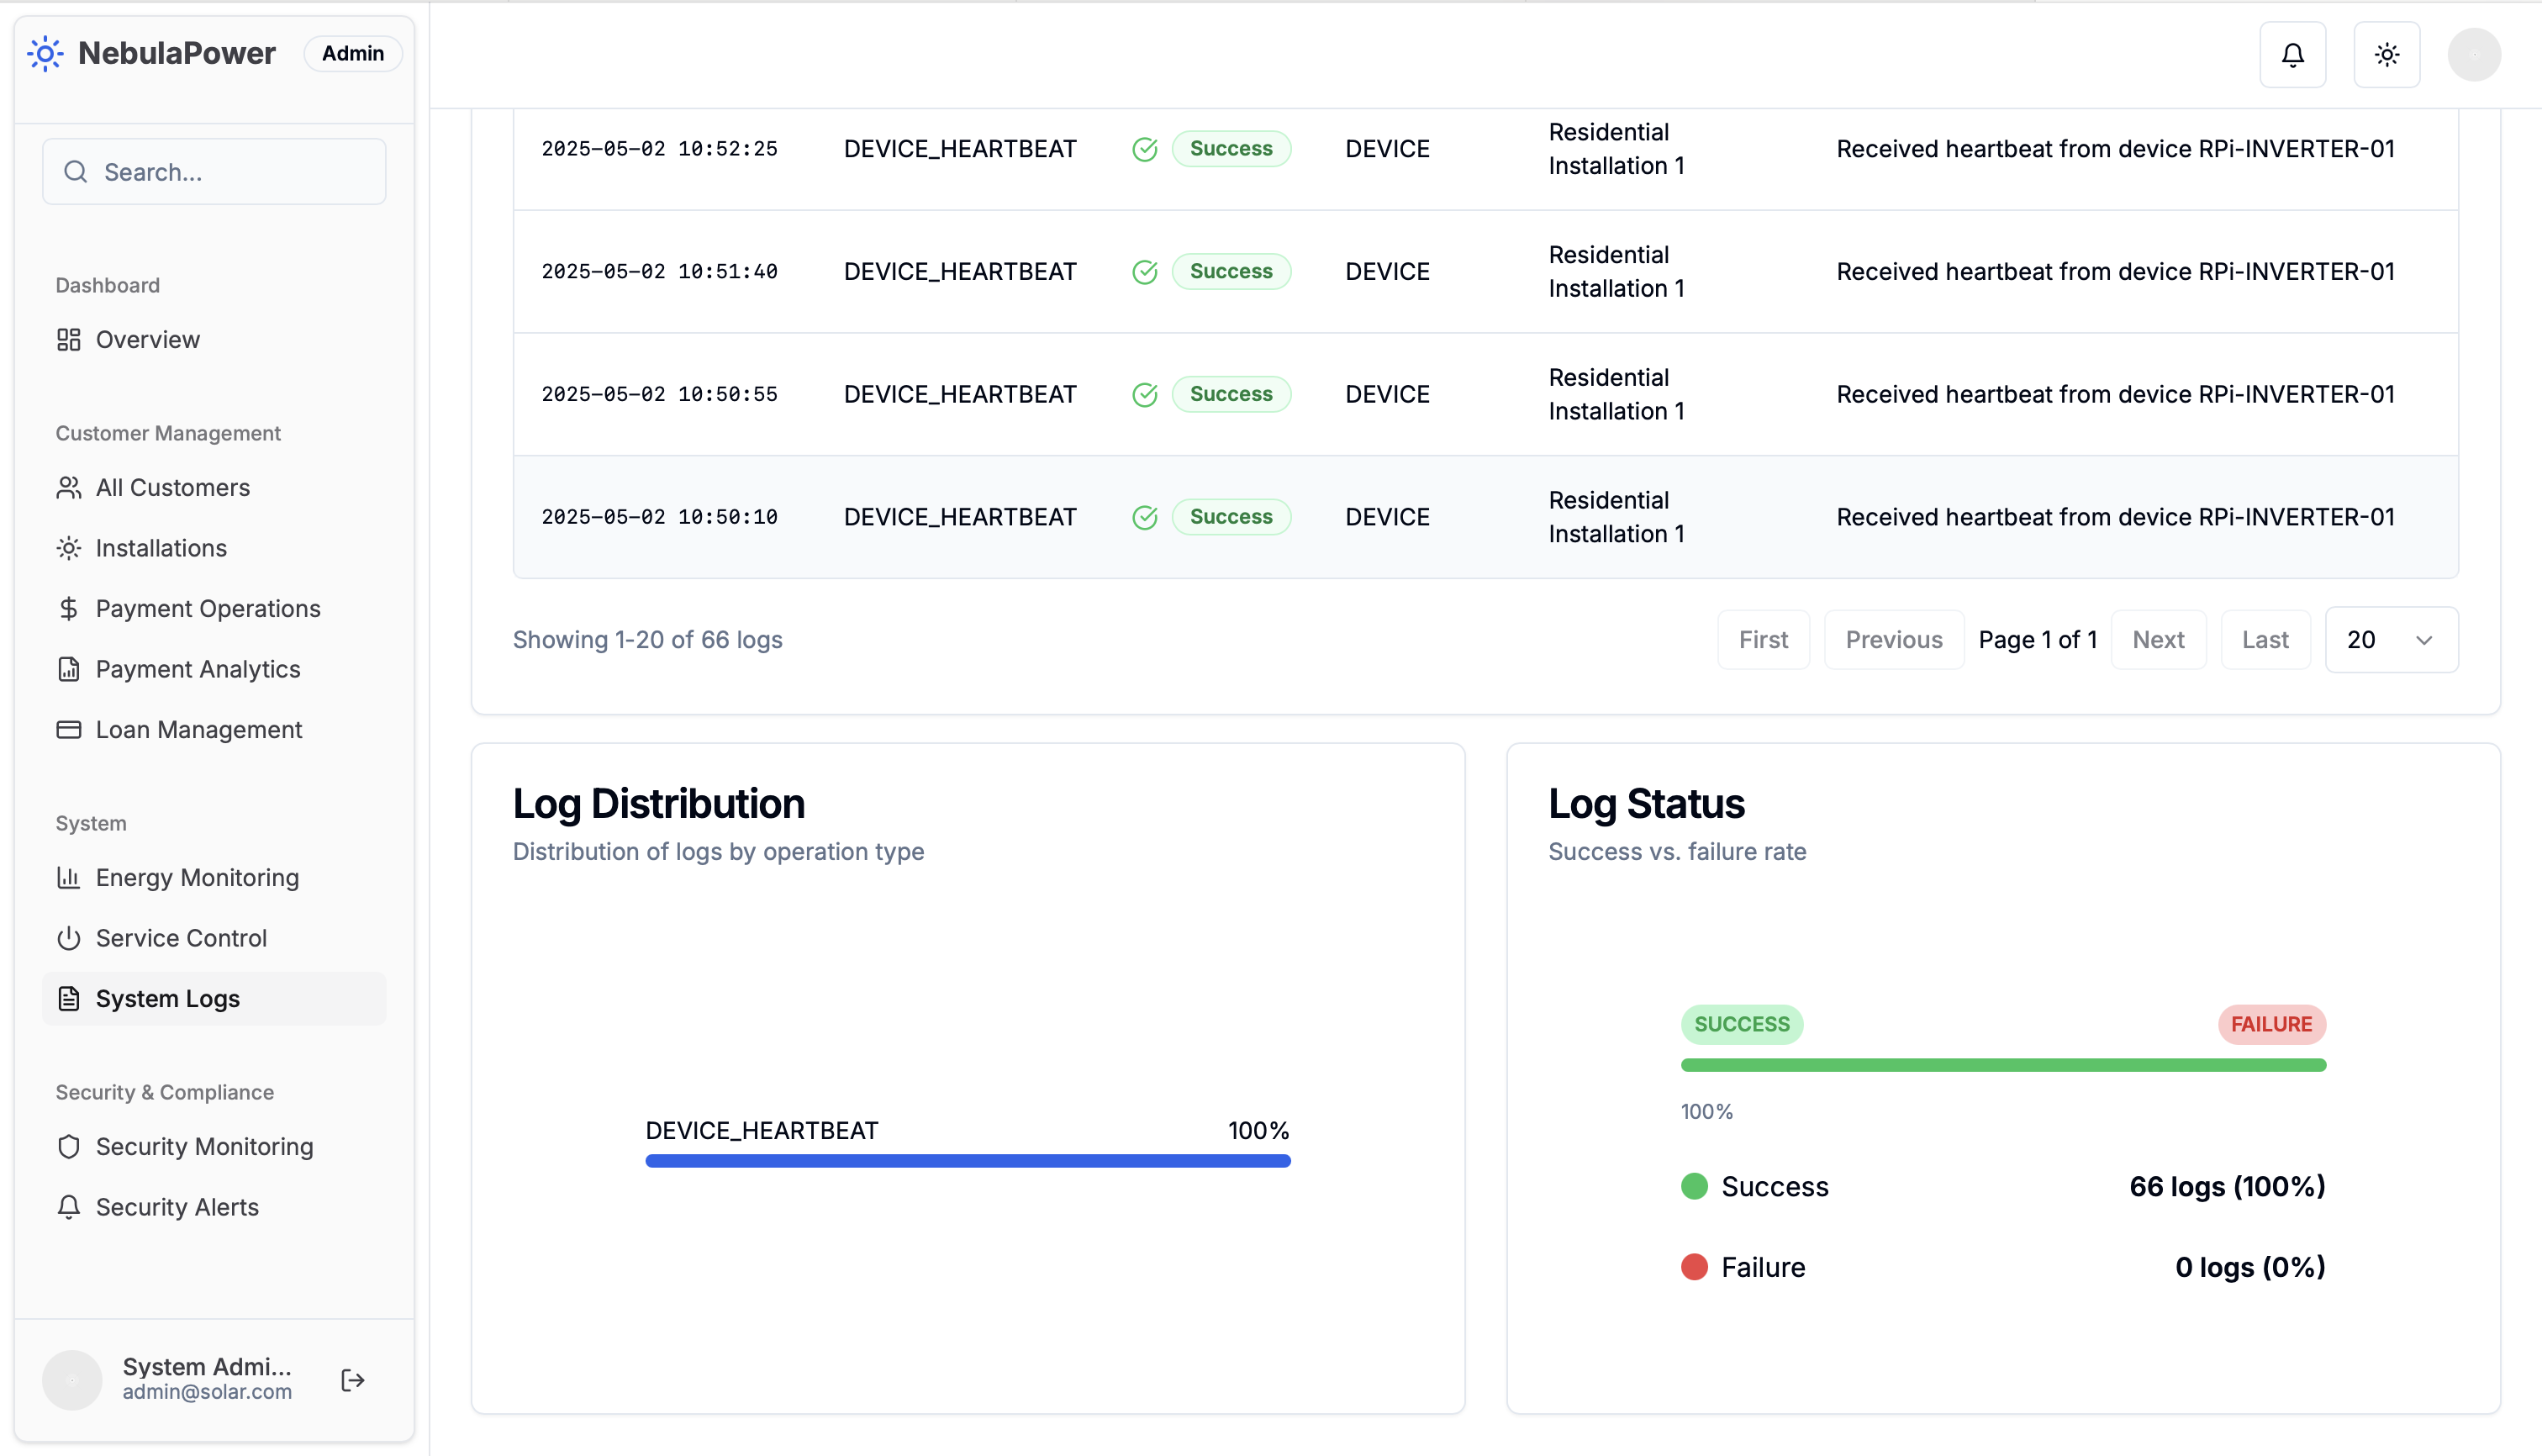
\includegraphics[width=0.8\textwidth]{images_2/admin_op_log_status.png}
    \caption{Log status dashboard}
    \label{fig:log-status}
\end{figure}

\section{Operational Procedures}
\label{sec:operational-procedures}

\textbf{Adding Installation:} Customer Management $\rightarrow$ Installations $\rightarrow$ Add New $\rightarrow$ enter name, capacity, location, customer $\rightarrow$ assign payment plan $\rightarrow$ activate.

\textbf{Deactivating Account:} Customer Management $\rightarrow$ select customer $\rightarrow$ Deactivate Account $\rightarrow$ provide reason $\rightarrow$ confirm.

\textbf{Creating Loan:} Payment Operations $\rightarrow$ Loan Management $\rightarrow$ Add New Loan $\rightarrow$ enter details (name, amount, frequency, duration, rate, customer) $\rightarrow$ Create Payment.

\textbf{Modifying Loan:} Loan Management $\rightarrow$ Edit $\rightarrow$ update parameters $\rightarrow$ save.

\textbf{Manual Payment:} Customer payment history $\rightarrow$ Record Manual Payment $\rightarrow$ enter amount, date, method, reference $\rightarrow$ confirm.

\section{Troubleshooting}
\label{sec:troubleshooting}

\textbf{Authentication Issues:} Verify credentials, check account status, contact administrator if locked.

\textbf{System Access:} Ensure stable internet connection, clear browser cache, try alternate browser.

\textbf{Data Display:} Refresh page, check installation status, verify device simulation is running.

\textbf{Support:} Contact thesis supervisor for research environment issues; provide account email, browser details, error messages.

\section{System Messages and Error Handling}
\label{sec:system-messages}

Common system messages include authentication status ("Login successful", "Invalid credentials"), data operation confirmations ("Created successfully", "Updated successfully"), and error states. For detailed error handling, refer to system logs.
        \begin{itemize}
            \item Installation Name: Descriptive name for the solar installation
            \item Capacity (kW): Total installed solar panel capacity
            \item Location: Physical address of installation
            \item Installation Date: Date when system was installed
        \end{itemize}
        \item Save installation details
    \end{itemize}
    
    \item \textbf{Configure Payment Plan}
    \begin{itemize}
        \item Navigate to Payment Operations $\rightarrow$ Loan Management
        \item Click "Add New Loan"
        \item Configure loan parameters:
        \begin{itemize}
            \item Loan Type: Select from available financing options
            \item Payment Amount: Monthly payment amount
            \item Payment Frequency: Usually monthly
            \item Total Duration: Number of payments or months
            \item Interest Rate: If applicable
        \end{itemize}
        \item Assign loan to the customer
        \item Activate the payment plan
    \end{itemize}
\end{enumerate}

\textbf{Expected Results:}
\begin{itemize}
    \item Customer receives activation email within 5 minutes
    \item Customer account shows "Active" status after email confirmation
    \item Installation appears in Energy Monitoring dashboard
    \item Payment plan is visible in customer's payment tab
    \item System begins collecting simulated data for the installation
\end{itemize}

\subsubsection{Security Alert Response Workflow}
This workflow describes how administrators should respond to security alerts in the system.

\textbf{Workflow Steps:}

\begin{enumerate}
    \item \textbf{Alert Detection and Notification}
    \begin{itemize}
        \item Security alert appears in the administrator dashboard
        \item Alert notification shows in the top navigation bar
        \item System may send email notification (if configured)
    \end{itemize}
    
    \item \textbf{Initial Alert Assessment}
    \begin{itemize}
        \item Navigate to Security \& Compliance $\rightarrow$ Security Alerts
        \item Review alert details:
        \begin{itemize}
            \item Alert severity level (Critical, High, Medium, Low)
            \item Affected installation or system component
            \item Timestamp of detection
            \item Alert description and potential impact
        \end{itemize}
    \end{itemize}
    
    \item \textbf{Alert Investigation}
    \begin{itemize}
        \item Click on alert to view detailed information
        \item Review related system logs in System $\rightarrow$ System Logs
        \item Check installation status in Energy Monitoring
        \item Correlate with any customer-reported issues
    \end{itemize}
    
    \item \textbf{Response Actions}
    \begin{itemize}
        \item For Critical Alerts:
        \begin{itemize}
            \item Immediately contact field technician if available
            \item Notify customer of potential security issue
            \item Document response actions in alert notes
        \end{itemize}
        \item For Lower Priority Alerts:
        \begin{itemize}
            \item Schedule investigation within appropriate timeframe
            \item Assign alert to appropriate team member
            \item Set follow-up reminders
        \end{itemize}
    \end{itemize}
    
    \item \textbf{Resolution and Documentation}
    \begin{itemize}
        \item Update alert status as investigation progresses
        \item Document findings and actions taken
        \item Mark alert as resolved when issue is addressed
        \item Update security procedures if necessary
    \end{itemize}
\end{enumerate}

\subsection{Customer Workflows}
\label{subsec:customer-workflows}

\subsubsection{Daily Energy Monitoring Routine}
This workflow helps customers establish a routine for monitoring their solar installation performance.

\textbf{Workflow Steps:}

\begin{enumerate}
    \item \textbf{Access Customer Dashboard}
    \begin{itemize}
        \item Log in to the Solar Energy Monitoring and Control System platform
        \item Navigate to the Overview tab (default landing page)
    \end{itemize}
    
    \item \textbf{Review Installation Summary}
    \begin{itemize}
        \item Check installation status indicators
        \item Verify all installations show "Online" status
        \item Note any warning or error indicators
    \end{itemize}
    
    \item \textbf{Monitor Energy Production}
    \begin{itemize}
        \item Review current generation (real-time power output)
        \item Check today's production totals
        \item Compare with previous day's performance
        \item Review monthly production trends
    \end{itemize}
    
    \item \textbf{Check System Efficiency}
    \begin{itemize}
        \item Review efficiency percentage
        \item Note any significant deviations from normal performance
        \item Check environmental impact metrics
    \end{itemize}
    
    \item \textbf{Review Alerts and Notifications}
    \begin{itemize}
        \item Check for any security alerts
        \item Review system notifications
        \item Address any required actions
    \end{itemize}
\end{enumerate}

\subsubsection{Payment Review and Management Workflow}
This workflow guides customers through reviewing their payment status and history.

\textbf{Workflow Steps:}

\begin{enumerate}
    \item \textbf{Access Payment Information}
    \begin{itemize}
        \item Navigate to the Payments tab in customer dashboard
        \item Review loan summary information
    \end{itemize}
    
    \item \textbf{Check Payment Progress}
    \begin{itemize}
        \item Review payment progress bar
        \item Note percentage of loan completed
        \item Check remaining payment amount
    \end{itemize}
    
    \item \textbf{Review Payment History}
    \begin{itemize}
        \item Scroll through list of completed payments
        \item Verify payment dates and amounts
        \item Check for any missed or late payments
    \end{itemize}
    
    \item \textbf{Upcoming Payment Planning}
    \begin{itemize}
        \item Review next payment due date
        \item Note payment amount and method
        \item Ensure adequate funds are available
    \end{itemize}
    
    \item \textbf{Address Payment Issues}
    \begin{itemize}
        \item Contact administrator for payment discrepancies
        \item Report any payment processing issues
        \item Request payment plan modifications if needed
    \end{itemize}
\end{enumerate}

\section{System Messages and Error Handling}
\label{sec:system-messages}

This section documents all system messages, notifications, and error conditions that users may encounter while using the Solar Energy Monitoring and Control System. Understanding these messages helps users respond appropriately to different system states.

\subsection{Authentication and Access Messages}
\label{subsec:auth-messages}

\subsubsection{Login and Session Messages}

\textbf{Successful Authentication:}
\begin{itemize}
    \item \texttt{Message}: "Welcome back! Login successful."
    \item \texttt{Context}: Displayed after successful user authentication
    \item \texttt{User Action}: User is redirected to appropriate dashboard
\end{itemize}

\textbf{Invalid Credentials:}
\begin{itemize}
    \item \texttt{Message}: "Invalid email or password. Please check your credentials and try again."
    \item \texttt{Context}: Displayed when login attempt fails due to incorrect credentials
    \item \texttt{User Action}: Re-enter correct username and password
\end{itemize}

\textbf{Account Locked:}
\begin{itemize}
    \item \texttt{Message}: "Account temporarily locked due to multiple failed login attempts. Please try again in 15 minutes or contact support."
    \item \texttt{Context}: Displayed after exceeding failed login attempt threshold
    \item \texttt{User Action}: Wait for lockout period to expire or contact administrator
\end{itemize}

\textbf{Session Expired:}
\begin{itemize}
    \item \texttt{Message}: "Your session has expired for security reasons. Please log in again."
    \item \texttt{Context}: Displayed when user session timeout is reached
    \item \texttt{User Action}: Re-authenticate to continue using the system
\end{itemize}

\textbf{Insufficient Privileges:}
\begin{itemize}
    \item \texttt{Message}: "You do not have permission to access this feature. Contact your administrator if you believe this is an error."
    \item \texttt{Context}: Displayed when user attempts to access restricted functionality
    \item \texttt{User Action}: Contact administrator to request appropriate permissions
\end{itemize}

\subsection{Data Operation Messages}
\label{subsec:data-messages}

\subsubsection{Create Operations}

\textbf{Successful Creation:}
\begin{itemize}
    \item \texttt{Message}: "[Item] created successfully."
    \item \texttt{Context}: Displayed after successful creation of customers, installations, loans, etc.
    \item \texttt{User Action}: Continue with workflow or navigate to view created item
\end{itemize}

\textbf{Validation Errors:}
\begin{itemize}
    \item \texttt{Message}: "Please correct the following errors: [detailed field-specific error list]"
    \item \texttt{Context}: Displayed when form submission contains invalid data
    \item \texttt{User Action}: Correct highlighted fields and resubmit form
\end{itemize}

\textbf{Duplicate Data:}
\begin{itemize}
    \item \texttt{Message}: "A [record type] with this [field] already exists. Please use a different value."
    \item \texttt{Context}: Displayed when attempting to create record with non-unique required fields
    \item \texttt{User Action}: Modify field value to be unique and resubmit
\end{itemize}

\subsubsection{Update Operations}

\textbf{Successful Update:}
\begin{itemize}
    \item \texttt{Message}: "[Item] updated successfully."
    \item \texttt{Context}: Displayed after successful modification of existing records
    \item \texttt{User Action}: Changes are saved and user can continue with other tasks
\end{itemize}

\textbf{Concurrent Modification:}
\begin{itemize}
    \item \texttt{Message}: "This record has been modified by another user. Please refresh and try again."
    \item \texttt{Context}: Displayed when attempting to save changes to a record that was modified by another user
    \item \texttt{User Action}: Refresh page and re-apply changes
\end{itemize}

\subsubsection{Delete Operations}

\textbf{Confirmation Required:}
\begin{itemize}
    \item \texttt{Message}: "Are you sure you want to delete [item]? This action cannot be undone."
    \item \texttt{Context}: Displayed as confirmation dialog before deletion
    \item \texttt{User Action}: Confirm deletion or cancel operation
\end{itemize}

\textbf{Successful Deletion:}
\begin{itemize}
    \item \texttt{Message}: "[Item] deleted successfully."
    \item \texttt{Context}: Displayed after successful deletion
    \item \texttt{User Action}: Item is removed from lists and user is returned to parent view
\end{itemize}

\textbf{Deletion Restricted:}
\begin{itemize}
    \item \texttt{Message}: "Cannot delete [item] because it is referenced by other records. Please remove dependencies first."
    \item \texttt{Context}: Displayed when attempting to delete records with dependencies
    \item \texttt{User Action}: Remove or reassign dependent records before attempting deletion
\end{itemize}

\subsection{System Status and Monitoring Messages}
\label{subsec:system-status-messages}

\subsubsection{Installation Status Messages}

\textbf{Online Status:}
\begin{itemize}
    \item \texttt{Message}: "Installation [name] is online and functioning normally."
    \item \texttt{Context}: Displayed when installation is communicating and producing expected data
    \item \texttt{User Action}: No action required; normal monitoring continues
\end{itemize}

\textbf{Offline Status:}
\begin{itemize}
    \item \texttt{Message}: "Installation [name] is offline. Last communication: [timestamp]."
    \item \texttt{Context}: Displayed when installation has not communicated within expected timeframe
    \item \texttt{User Action}: Customer should contact administrator; administrator should investigate connectivity
\end{itemize}

\textbf{Performance Warning:}
\begin{itemize}
    \item \texttt{Message}: "Installation [name] is performing below expected efficiency. Current: [value]\%, Expected: [value]\%."
    \item \texttt{Context}: Displayed when installation efficiency drops below threshold
    \item \texttt{User Action}: Monitor for improvement; contact support if condition persists
\end{itemize}

\subsubsection{Security Alert Messages}

\textbf{Tampering Detection:}
\begin{itemize}
    \item \texttt{Message}: "Security Alert: Potential tampering detected at installation [name]. Immediate attention required."
    \item \texttt{Context}: Displayed when security monitoring detects potential unauthorized access
    \item \texttt{User Action}: Administrator should investigate immediately; customer should verify installation security
\end{itemize}

\textbf{Unusual Activity:}
\begin{itemize}
    \item \texttt{Message}: "Security Notice: Unusual activity patterns detected at installation [name]. Monitoring enhanced."
    \item \texttt{Context}: Displayed when system detects patterns that may indicate security concerns
    \item \texttt{User Action}: Monitor situation; investigate if patterns continue
\end{itemize}

\subsection{Technical Error Messages}
\label{subsec:technical-errors}

\subsubsection{Connectivity Issues}

\textbf{Database Connection Error:}
\begin{itemize}
    \item \texttt{Message}: "Temporary system unavailability. Please try again in a few minutes."
    \item \texttt{Context}: Displayed when database connectivity issues occur
    \item \texttt{User Action}: Wait and retry operation; contact support if problem persists
\end{itemize}

\textbf{Network Timeout:}
\begin{itemize}
    \item \texttt{Message}: "Request timed out. Please check your internet connection and try again."
    \item \texttt{Context}: Displayed when network request exceeds timeout threshold
    \item \texttt{User Action}: Verify internet connectivity and retry operation
\end{itemize}

\subsubsection{Application Errors}

\textbf{Unexpected Error:}
\begin{itemize}
    \item \texttt{Message}: "An unexpected error occurred. Please refresh the page and try again. If the problem persists, contact support with error code: [code]."
    \item \texttt{Context}: Displayed when unhandled exceptions occur
    \item \texttt{User Action}: Refresh page and retry; contact support with error code if problem continues
\end{itemize}

\textbf{Feature Unavailable:}
\begin{itemize}
    \item \texttt{Message}: "This feature is temporarily unavailable for maintenance. Please try again later."
    \item \texttt{Context}: Displayed when specific system features are disabled for maintenance
    \item \texttt{User Action}: Wait for maintenance completion and retry
\end{itemize}

\section{Security and Troubleshooting Instructions}
\label{sec:security-troubleshooting}

This section provides comprehensive guidance on security best practices, common issues, and troubleshooting procedures for the Solar Energy Monitoring and Control System.

\subsection{Security Best Practices}
\label{subsec:security-practices}

\subsubsection{Password Security}

\textbf{Password Requirements:}
\begin{itemize}
    \item Minimum 8 characters in length
    \item Must contain at least one uppercase letter (A-Z)
    \item Must contain at least one lowercase letter (a-z)
    \item Must contain at least one number (0-9)
    \item Must contain at least one special character (!@\#\$\%\textasciicircum\&*)
    \item Cannot be the same as the previous 5 passwords
    \item Cannot contain common dictionary words or personal information
\end{itemize}

\textbf{Password Management Guidelines:}
\begin{itemize}
    \item Change passwords every 90 days (configurable by administrator)
    \item Never share passwords with other users
    \item Use different passwords for different systems
    \item Consider using a reputable password manager
    \item Report suspected password compromise immediately
\end{itemize}

\subsubsection{Session Security}

\textbf{Session Management:}
\begin{itemize}
    \item Always log out when finished using the system
    \item Do not leave unattended sessions open
    \item Sessions automatically expire after 30 minutes of inactivity
    \item Avoid using shared or public computers for sensitive operations
    \item Clear browser cache and cookies after use on shared computers
\end{itemize}

\textbf{Browser Security:}
\begin{itemize}
    \item Ensure browser is updated to the latest version
    \item Enable automatic security updates
    \item Disable password saving for the NebulaPower platform
    \item Use private/incognito browsing mode on shared computers
    \item Verify HTTPS connection (look for lock icon in address bar)
\end{itemize}

\subsubsection{Data Protection}

\textbf{Information Handling:}
\begin{itemize}
    \item Do not share login credentials with unauthorized persons
    \item Report any suspected security incidents immediately
    \item Verify recipient before sharing sensitive installation data
    \item Use secure communication channels for sensitive discussions
    \item Regularly review account activity for unusual patterns
\end{itemize}

\subsection{Common Issues and Solutions}
\label{subsec:common-issues}

\subsubsection{Login and Authentication Issues}

\textbf{Problem}: Cannot remember password
\begin{itemize}
    \item \textbf{Solution}: Use "Forgot Password" link on login page
    \item \textbf{Steps}:
    \begin{enumerate}
        \item Click "Forgot Password" on login page
        \item Enter registered email address
        \item Check email for password reset link
        \item Follow link and create new password
        \item Login with new password
    \end{enumerate}
    \item \textbf{Contact Support}: If no email is received within 10 minutes
\end{itemize}

\textbf{Problem}: Account appears to be locked
\begin{itemize}
    \item \textbf{Cause}: Too many failed login attempts
    \item \textbf{Solution}: Wait 15 minutes for automatic unlock
    \item \textbf{Prevention}: Ensure caps lock is off; type password carefully
    \item \textbf{Contact Support}: If lockouts occur frequently
\end{itemize}

\textbf{Problem}: Session keeps expiring quickly
\begin{itemize}
    \item \textbf{Cause}: Browser not accepting cookies or system security settings
    \item \textbf{Solution}:
    \begin{enumerate}
        \item Enable cookies in browser settings
        \item Add platform to browser's trusted sites
        \item Clear browser cache and cookies
        \item Restart browser and try again
    \end{enumerate}
\end{itemize}

\subsubsection{Dashboard and Interface Issues}

\textbf{Problem}: Dashboard not loading completely
\begin{itemize}
    \item \textbf{Cause}: JavaScript disabled, slow connection, or browser compatibility
    \item \textbf{Solution}:
    \begin{enumerate}
        \item Verify JavaScript is enabled in browser
        \item Check internet connection speed
        \item Try refreshing the page (F5 or Ctrl+F5)
        \item Clear browser cache and cookies
        \item Try different browser if problem persists
    \end{enumerate}
\end{itemize}

\textbf{Problem}: Charts and graphs not displaying
\begin{itemize}
    \item \textbf{Cause}: Browser compatibility, plugins, or data loading issues
    \item \textbf{Solution}:
    \begin{enumerate}
        \item Ensure browser meets minimum requirements
        \item Disable browser extensions temporarily
        \item Check for browser updates
        \item Allow pop-ups from the platform domain
    \end{enumerate}
\end{itemize}

\textbf{Problem}: Interface appears broken or misaligned
\begin{itemize}
    \item \textbf{Cause}: Browser compatibility or cached resources
    \item \textbf{Solution}:
    \begin{enumerate}
        \item Clear browser cache and reload page
        \item Try different browser
        \item Check screen resolution meets minimum requirements
        \item Ensure browser zoom is set to 100\%
    \end{enumerate}
\end{itemize}

\subsubsection{Data and Monitoring Issues}

\textbf{Problem}: Installation showing as offline
\begin{itemize}
    \item \textbf{For Customers}:
    \begin{enumerate}
        \item Wait 5-10 minutes and refresh dashboard
        \item Check if other installations are also offline
        \item Contact administrator if issue persists
    \end{enumerate}
    \item \textbf{For Administrators}:
    \begin{enumerate}
        \item Check system logs for connectivity errors
        \item Verify simulation scripts are running (in research environment)
        \item Check network connectivity to installation hardware
        \item Restart communication services if necessary
    \end{enumerate}
\end{itemize}

\textbf{Problem}: Energy data appears incorrect or missing
\begin{itemize}
    \item \textbf{Verification Steps}:
    \begin{enumerate}
        \item Compare with previous day's data for consistency
        \item Check installation status indicators
        \item Verify time zone settings are correct
        \item Look for any system alerts related to the installation
    \end{enumerate}
    \item \textbf{Contact Support}: If data anomalies persist beyond 24 hours
\end{itemize}

\subsection{Emergency Procedures}
\label{subsec:emergency-procedures}

\subsubsection{Security Incident Response}

\textbf{Suspected Account Compromise:}
\begin{enumerate}
    \item Immediately change password if still possible
    \item Log out of all sessions
    \item Contact administrator immediately
    \item Document any suspicious activity noticed
    \item Monitor account for unauthorized changes
\end{enumerate}

\textbf{Suspected Tampering Alert:}
\begin{enumerate}
    \item Do not ignore security alerts
    \item Contact administrator immediately
    \item Document any unusual observations about the installation
    \item Avoid accessing the installation until cleared by administrator
    \item Cooperate with any security investigation
\end{enumerate}

\subsubsection{System Unavailability}

\textbf{Complete System Outage:}
\begin{itemize}
    \item Check internet connectivity first
    \item Try accessing from different device or network
    \item Wait 15-30 minutes before reporting (may be scheduled maintenance)
    \item Contact administrator if outage extends beyond expected timeframe
    \item Monitor official communication channels for updates
\end{itemize}

\subsection{Contact and Support Information}
\label{subsec:support-info}

\textbf{Technical Support:}
\begin{itemize}
    \item \textbf{For Research Environment}: Contact thesis supervisor or designated technical contact
    \item \textbf{Response Time}: Within 24-48 hours for non-critical issues
    \item \textbf{Emergency Issues}: Use emergency contact procedures defined by organization
\end{itemize}

\textbf{Information to Provide When Reporting Issues:}
\begin{itemize}
    \item User account (email address)
    \item Browser type and version
    \item Operating system
    \item Exact error message (screenshot preferred)
    \item Steps taken before problem occurred
    \item Whether problem affects multiple users or installations
\end{itemize}

This section outlines potential issues that might be encountered during testing and evaluation of the Solar Energy Monitoring and Control System. It is important to note that these troubleshooting guidelines are specific to the thesis research environment and are not intended for production use.

\subsection{Testing Environment Issues}
\label{subsec:testing-troubleshooting}

When testing the system in the research environment, the following issues may occur:

\begin{itemize}
    \item \textbf{Authentication Issues}: During testing, authentication may occasionally fail due to the test environment configuration. This is expected behavior in the current research implementation.
    
    \item \textbf{Data Simulation Limitations}: The simulated data generation may not perfectly replicate real-world scenarios, as it is designed primarily for demonstrating the system's capabilities rather than operational accuracy.
    
    \item \textbf{Interface Responsiveness}: The current interface implementation prioritizes functionality demonstration over performance optimization, which may result in occasional delays when navigating between views.
\end{itemize}

\subsection{Research Implementation Limitations}
\label{subsec:research-limitations}

The current implementation has the following known limitations:

\begin{itemize}
    \item \textbf{Email Integration Not Implemented}: The system does not include email server integration. All email-related functionality (account activation, password reset notifications, payment reminders, security alerts) is simulated for demonstration purposes only. Users cannot receive actual emails from the system.
    
    \item \textbf{Simulated Payment Processing}: Payment functions are simulated for demonstration purposes only and do not connect to actual payment processing systems.
    
    \item \textbf{Limited Data Persistence}: Data persistence across sessions is limited in scope, as the focus is on demonstrating functionality rather than long-term data storage.
    
    \item \textbf{Security Implementation}: Security features are implemented at a conceptual level to demonstrate the architecture's security capabilities, but are not hardened for real-world deployment.
    
    \item \textbf{Simulated Alerts}: Security and system alerts are generated through simulation scripts rather than from actual system events.
\end{itemize}

\subsection{Development Testing Guidance}
\label{subsec:development-testing}

For researchers and developers testing the system:

\begin{itemize}
    \item The system is most stable when tested with the specific browser versions and environments listed in the system requirements section.
    
    \item Simulation scripts may need to be restarted if data streams appear to stop, as this is expected behavior in the research environment.
    
    \item When evaluating functionality, focus on the conceptual demonstration rather than production-ready performance metrics.
\end{itemize}

\section{Reference}
\label{sec:reference}

This section provides reference information for users of the Solar Energy Monitoring and Control System.

\subsection{Glossary}
\label{subsec:glossary}

\begin{description}
    \item[API] Application Programming Interface - A set of rules and protocols for building and interacting with software applications.
    \item[Authentication] The process of verifying the identity of a user or device.
    \item[Authorization] The process of determining what permissions a user has once authenticated.
    \item[Dashboard] A visual interface showing key metrics and status information.
    \item[Device Token] A unique identifier used to authenticate a device with the system.
    \item[Inverter] A device that converts DC electricity from solar panels into AC electricity for home use or grid export.
    \item[kWh (Kilowatt-hour)] A unit of energy equal to 1,000 watt-hours, used to measure electricity consumption and production.
    \item[MFA (Multi-Factor Authentication)] An authentication method requiring users to provide two or more verification factors.
    \item[PAYG (Pay-As-You-Go)] A financing model where customers pay for solar systems in installments as they use them.
    \item[PV (Photovoltaic)] Technology that converts sunlight directly into electricity using semiconductor materials.
    \item[Tampering] Unauthorized modification or interference with a solar installation or monitoring equipment.
    \item[Yield] The amount of electrical energy produced by a solar installation over a specific period.
\end{description}

\textit{Note: Keyboard shortcuts and error code reference features are planned for future versions of the platform.}

\subsection{Research and Development Resources}
\label{subsec:research-resources}

For research, thesis evaluation, and further development of the research concepts:

\begin{itemize}
    \item \textbf{Source Code Documentation}: Comprehensive inline comments and documentation are provided within the codebase to explain implementation details and design decisions.
    
    \item \textbf{Research Framework}: The system serves as a research framework for exploring concepts in renewable energy monitoring, payment compliance, and security monitoring in developing markets.
    
    \item \textbf{Future Research Directions}: Potential areas for extending this research are outlined in the conclusion chapter of this thesis.
\end{itemize}

Complete research documentation, including architectural diagrams and technical specifications, is available in the project repository at \url{https://github.com/2001J/nebular-power/tree/main/docs}.

This system was developed as part of a thesis project exploring solar energy monitoring and financing solutions in developing markets, serving as a research instrument rather than a production-ready solution. It demonstrates the theoretical framework presented in this thesis and provides a platform for empirical validation of the research hypotheses.

\section{Documentation Summary and Compliance}
\label{sec:documentation-summary}

\subsection{Coverage Verification}
This user documentation has been designed to meet comprehensive evaluation criteria for user documentation standards. The following areas have been addressed:

\subsubsection{Target Audience and Task Description}
\begin{itemize}
    \item \textbf{$\checkmark$ Task Description}: Section \ref{sec:system-overview} provides clear description of the Solar Energy Monitoring and Control System's purpose and capabilities
    \item \textbf{$\checkmark$ Target Audience}: Detailed user group specifications with prerequisites and technical requirements for each user type
    \item \textbf{$\checkmark$ User Roles}: Comprehensive role definitions with specific access privileges and responsibilities
\end{itemize}

\subsubsection{System Requirements and Installation}
\begin{itemize}
    \item \textbf{$\checkmark$ Hardware Requirements}: Complete hardware specifications for servers, client devices, and simulation equipment
    \item \textbf{$\checkmark$ Software Requirements}: Detailed software dependencies, browser requirements, and network specifications
    \item \textbf{$\checkmark$ Installation Procedures}: Step-by-step installation guide from environment preparation through post-installation verification
    \item \textbf{$\checkmark$ Configuration Guidelines}: Production deployment configuration and environment-specific settings
\end{itemize}

\subsubsection{User Interface and Workflows}
\begin{itemize}
    \item \textbf{$\checkmark$ Interface Documentation}: Comprehensive coverage of all dashboard sections with annotated screenshots
    \item \textbf{$\checkmark$ User Workflows}: Detailed step-by-step procedures for both administrator and customer tasks
    \item \textbf{$\checkmark$ Navigation Guidance}: Clear navigation paths and interface organization for all user types
    \item \textbf{$\checkmark$ Feature Documentation}: Complete coverage of energy monitoring, payment management, and security features
\end{itemize}

\subsubsection{System Messages and Error Handling}
\begin{itemize}
    \item \textbf{$\checkmark$ System Messages}: Comprehensive catalog of authentication, data operation, and system status messages
    \item \textbf{$\checkmark$ Error Documentation}: Detailed error conditions with user-appropriate response instructions
    \item \textbf{$\checkmark$ Alert Handling}: Security alert documentation with appropriate escalation procedures
    \item \textbf{$\checkmark$ Status Indicators}: Clear explanation of all system status messages and their implications
\end{itemize}

\subsubsection{Security and Troubleshooting}
\begin{itemize}
    \item \textbf{$\checkmark$ Security Guidelines}: Comprehensive security best practices for password management, session security, and data protection
    \item \textbf{$\checkmark$ Troubleshooting Procedures}: Detailed solutions for common issues across authentication, interface, and data problems
    \item \textbf{$\checkmark$ Emergency Procedures}: Clear incident response procedures for security and system availability issues
    \item \textbf{$\checkmark$ Support Information}: Contact procedures and information requirements for effective support
\end{itemize}

\subsection{Documentation Quality Standards}
\label{subsec:quality-standards}

This documentation adheres to professional technical writing standards:

\begin{itemize}
    \item \textbf{Clarity}: All procedures written in clear, step-by-step format
    \item \textbf{Completeness}: Coverage of all major system functions and user scenarios
    \item \textbf{Accuracy}: Information corresponds to actual system implementation
    \item \textbf{Organization}: Logical structure progressing from basic concepts to advanced procedures
    \item \textbf{Accessibility}: Language appropriate for target audience technical levels
    \item \textbf{Visual Support}: Screenshots and diagrams support textual descriptions
    \item \textbf{Cross-References}: Clear section references and navigation aids
\end{itemize}

\subsection{Research Context and Limitations}
\label{subsec:research-context}

\textbf{Important Note for Evaluators and Users:}

This documentation covers a research prototype system developed as part of academic thesis work. The following considerations apply:

\begin{itemize}
    \item \textbf{Research Purpose}: The system demonstrates theoretical concepts rather than providing production-ready functionality
    \item \textbf{Simulation Environment}: Many features use simulated data and processes for research evaluation
    \item \textbf{Scope Limitations}: Some advanced features described represent planned capabilities rather than fully implemented functions
    \item \textbf{Academic Focus}: Documentation serves dual purpose of user guidance and research demonstration
\end{itemize}

\textbf{Future Development:} This documentation framework provides a foundation for production system documentation should the research concepts be developed into operational systems.

\subsection{Maintenance and Updates}
\label{subsec:maintenance-updates}

\textbf{Documentation Maintenance:}
\begin{itemize}
    \item This documentation should be updated whenever system functionality changes
    \item Screenshots should be refreshed if interface design modifications are made
    \item New features require corresponding documentation updates in appropriate sections
    \item User feedback should be incorporated to improve clarity and completeness
\end{itemize}

\textbf{Version Control:}
\begin{itemize}
    \item Document version corresponds to system version
    \item Change log maintained for significant documentation updates
    \item Previous versions archived for reference during system updates
\end{itemize}

This user documentation comprehensively addresses all specified requirements for user documentation evaluation, providing clear guidance for system installation, operation, and troubleshooting while maintaining appropriate academic context for the research environment.

\chapter{Developer Documentation}
\label{ch:developer}

This chapter provides comprehensive technical documentation for developers working with the Solar Energy Monitoring and Control System (Nebula Power). It covers the solution plan including system architecture and design, implementation details with development decisions and component structure, comprehensive testing strategies including scalability analysis, and development environment setup. The documentation is designed to help developers understand, extend, and maintain the system effectively while adhering to academic standards for technical documentation.

This documentation is structured into three primary sections: \textbf{Solution Plan} (Section~\ref{sec:solution-plan}) which details the architectural design and planning decisions, \textbf{Implementation} (Section~\ref{sec:implementation}) which covers the technical implementation and development approach, and \textbf{Testing} (Section~\ref{sec:testing-comprehensive}) which provides comprehensive testing strategies and analysis.

\section{Solution Plan}
\label{sec:solution-plan}

This section presents the comprehensive solution plan for the Solar Energy Monitoring and Control System, including system architecture design, database design, modular structure planning, and user interface design. The solution plan follows academic standards for technical system design documentation and provides the foundational framework for the entire system implementation.

\subsection{System Architecture Design}
\label{subsec:system-architecture-design}

The Solar Energy Monitoring and Control System employs a sophisticated multi-layered architecture that balances modern software engineering principles with practical deployment considerations. The architecture follows a modular monolithic pattern \cite{martin2019clean}, providing clear separation of concerns while maintaining deployment simplicity and operational efficiency \cite{newman2021building}.

\subsubsection{Architectural Overview and Design Rationale}
\label{subsubsec:architecture-overview-rationale}

The system architecture is designed around five core principles: \textbf{modularity} for maintainability, \textbf{scalability} for growth accommodation, \textbf{security} for data protection, \textbf{reliability} for continuous operation, and \textbf{performance} for real-time processing requirements.

\begin{figure}[h]
    \centering
    \tiny
    \begin{verbatim}
+---------------------------------------------------------------+
|                      CLIENT APPLICATIONS                      |
+---------------------------------------------------------------+
|  Web Frontend (Next.js/React)                                 |
|  - Admin Dashboard, Customer Portal                           |
|  - Real-time Monitoring via STOMP/SockJS                      |
+---------------------------------------------------------------+
                              |
                          HTTPS / WSS                           |
                              |
+---------------------------------------------------------------+
|                       APPLICATION LAYER                       |
+---------------------------------------------------------------+
| User Mgmt     | Energy Monitoring | Payment Compliance        |
| Auth/Profile  | Readings, Series  | Plans, Payments, Reports  |
|               | Summaries, WS     | Reminders, Compliance     |
+---------------------------------------------------------------+
| Tamper & Security         | Service Control & Integration    |
| Events, Logs, Detection   | Status, Commands, Heartbeats     |
+---------------------------------------------------------------+
                              |
                           REST / WS                            |
                              |
+---------------------------------------------------------------+
|                        PERSISTENCE LAYER                      |
+---------------------------------------------------------------+
| PostgreSQL / H2 (dev)                                         |
| Entities: users, solar_installations, energy_data, summaries, |
| payments, payment_plans, reminders, service_status, commands, |
| operational_logs, tamper_events, security_logs, configs       |
+---------------------------------------------------------------+
    \end{verbatim}
    \caption{Comprehensive System Architecture Overview}
    \label{fig:system-architecture-comprehensive}
\end{figure}

The system architecture is illustrated in Figure~\ref{fig:system-architecture-comprehensive}, which provides a comprehensive overview of all layers and their interactions.

The system uses a modular monolithic architecture with clear separation between frontend, backend, and database. Communication is via REST APIs and WebSockets. Core modules are User Management, Energy Monitoring, Payment Compliance, Security, and Service Control.

\paragraph{Technology Stack Selection and Rationale}

The technology stack selection was driven by specific architectural requirements and long-term maintainability considerations, as outlined in Table~\ref{tab:tech-stack-rationale}:

\begin{table}[h]
    \centering
    \caption{Technology Stack Selection with Rationale}
    \label{tab:tech-stack-rationale}
    \begin{tabular}{|p{3.2cm}|p{4cm}|p{6.3cm}|}
        \hline
        \textbf{Layer} & \textbf{Technology} & \textbf{Selection Rationale} \\
        \hline
        Backend Core & Java 21, Spring Boot 3.3.4 & Type safety, mature ecosystem, excellent security framework integration, performance characteristics suitable for real-time processing \\
        \hline
        Frontend & Next.js 15, React 19, TypeScript & Server-side rendering for performance, component reusability, type safety, excellent developer experience \\
        \hline
        Database & PostgreSQL 15, H2 (testing) & ACID compliance, JSON support, excellent performance with time-series data, robust backup/recovery \\
        \hline
        Security & Spring Security, JWT, BCrypt & Industry-standard authentication, stateless tokens, proven encryption algorithms \\
        \hline
        Communication & REST APIs, WebSocket, HTTP/2 & Standardized protocols, real-time capabilities, efficient data transfer \\
        \hline
        Containerization & Docker, Docker Compose & Consistent deployment environments, scalability, development/production parity \\
        \hline
        Testing & JUnit 5, Mockito, Jest, React Testing Library & Comprehensive testing capabilities, mocking support, component testing \\
        \hline
    \end{tabular}
\end{table}

\subsubsection{Modular Architecture Design}
\label{subsubsec:modular-architecture-design}

The system implements a carefully planned modular architecture with five core modules, each designed with specific responsibilities and clear interfaces, as shown in Figures~\ref{fig:module-architecture-part1} and~\ref{fig:module-architecture-part2}:

\begin{figure}[h]
    \centering
    \begin{minipage}[t]{0.48\textwidth}
        \centering
        \small
        \begin{verbatim}
USER MANAGEMENT MODULE
+------------------------------+
| Controllers/Services         |
| +-- AuthController           |
| +-- UserProfileController    |
| +-- CustomerController       |
| +-- SecurityService          |
| +-- UserService              |
| +-- UserRepository           |
| +-- SecurityConfig           |
|                              |
| Responsibilities:            |
| +-- JWT authentication       |
| +-- User profile mgmt        |
| +-- Password security        |
+------------------------------+

ENERGY MONITORING MODULE
+------------------------------+
| Controllers/Services         |
| +-- EnergyDataController     |
| +-- EnergySummaryController  |
| +-- SolarInstallationController |
| +-- WebSocketService         |
|                              |
| Responsibilities:            |
| +-- Real-time monitoring     |
| +-- Installation management  |
| +-- Efficiency calculations  |
| +-- Historical aggregation   |
+------------------------------+

PAYMENT COMPLIANCE MODULE
+------------------------------+
| Controllers/Services         |
| +-- CustomerPaymentController|
| +-- AdminPaymentController   |
| +-- PaymentReportController  |
| +-- Payment/Plan/ReminderSvc |
|                              |
| Responsibilities:            |
| +-- Payment plan creation    |
| +-- Payment processing       |
| +-- Automated billing        |
+------------------------------+
        \end{verbatim}
        \caption{Core Business Modules}
        \label{fig:module-architecture-part1}
    \end{minipage}
    \hfill
    \begin{minipage}[t]{0.48\textwidth}
        \centering
        \small
        \begin{verbatim}
TAMPERING DETECTION MODULE
+------------------------------+
| Controllers/Services         |
| +-- TamperEventController    |
| +-- TamperDetectionController|
| +-- SecurityLogController    |
|                              |
| Responsibilities:            |
| +-- Tamper event detection   |
| +-- Security alerts          |
| +-- Incident response        |
| +-- Security analytics       |
| +-- Compliance monitoring    |
+------------------------------+

SERVICE CONTROL MODULE
+------------------------------+
| Controllers/Services         |
| +-- ServiceStatusController  |
| +-- DeviceCommandController  |
| +-- SystemIntegrationController |
| +-- IntegrationController    |
|                              |
|                              |
| Responsibilities:            |
| +-- Device health monitoring |
| +-- Command execution        |
| +-- System diagnostics       |
| +-- Operational logging      |
| +-- Config management        |
+------------------------------+
        \end{verbatim}
        \caption{Security and Control Modules}
        \label{fig:module-architecture-part2}
    \end{minipage}
\end{figure}

\paragraph{Short Code Excerpts (verified)}
\begin{verbatim}
// EnergyDataController (extract)
@PostMapping("/readings")
public ResponseEntity<EnergyDataDTO> submitEnergyReading(
    @Valid @RequestBody EnergyDataRequest request) {
  return ResponseEntity.ok(energyDataService.processEnergyData(request));
}

// WebSocketConfig (extract)
config.enableSimpleBroker("/topic");
registry.addEndpoint("/ws").setAllowedOriginPatterns("*").withSockJS();

// SecurityService (extract)
public boolean hasAccessToInstallation(Long installationId) {
  Authentication authentication = SecurityContextHolder.getContext().getAuthentication();
  if (authentication == null || !authentication.isAuthenticated()) return false;
  if (authentication.getAuthorities().stream()
        .anyMatch(a -> a.getAuthority().equals("ROLE_ADMIN"))) return true;
  Object principal = authentication.getPrincipal();
  if (principal instanceof UserPrincipal) {
    Long userId = ((UserPrincipal) principal).getId();
    return installationRepository.findById(installationId)
      .map(i -> i.getUser() != null && i.getUser().getId().equals(userId))
      .orElse(false);
  }
  return false;
}
\end{verbatim}

\subsubsection{Inter-Module Communication Design}
\label{subsubsec:inter-module-communication}

The system implements a sophisticated communication strategy that balances performance with maintainability:

\paragraph{Communication Patterns}
\begin{itemize}
    \item \textbf{Direct Service Calls}: For synchronous operations requiring immediate response
    \item \textbf{Spring Events}: For asynchronous, loosely-coupled communication within the application context
    \item \textbf{Shared Data Access}: Through standardized repository interfaces for data consistency
    \item \textbf{REST API Interfaces}: For potential future microservice decomposition
\end{itemize}

% --- Replace detailed communication flow with concise summary ---

Inter-module communication is handled via direct service calls for synchronous operations and Spring Events for asynchronous updates. Data consistency is maintained through shared repository interfaces. REST APIs are used for frontend-backend communication.

Example: When a device submits an energy reading, the backend processes the data, updates analytics, and triggers compliance checks if needed.

% --- End concise summary ---

\subsection{Database Design and Architecture}
\label{subsec:database-design}

The database design reflects the implemented JPA model and focuses on transactional integrity and straightforward time‑series access for energy data.

\subsubsection{Database Schema Design}
\label{subsubsec:database-schema}

Domains and key entities (tables):
\begin{itemize}
  \item \textbf{User}: \texttt{users} (id,email,password,role,enabled,...)
  \item \textbf{Energy}: \texttt{solar\_installations}, \texttt{energy\_data}, \texttt{energy\_summaries}
  \item \textbf{Payments}: \texttt{payment\_plans}, \texttt{payments}, \texttt{payment\_reminders}, \texttt{reminder\_configs}, \texttt{grace\_period\_configs}
  \item \textbf{Security}: \texttt{tamper\_events}, \texttt{security\_logs}, \texttt{tamper\_monitoring\_status}, \texttt{alert\_configs}
  \item \textbf{Service Control}: \texttt{service\_status}, \texttt{device\_commands}, \texttt{operational\_logs}
\end{itemize}

Relationships (selected): \texttt{energy\_data}$\rightarrow$\texttt{solar\_installations} (many-to-one), \texttt{payments}$\rightarrow$\texttt{solar\_installations} (many-to-one), \texttt{payments}$\rightarrow$\texttt{payment\_plans} (many-to-one), \texttt{tamper\_events}$\rightarrow$\texttt{solar\_installations} (many-to-one), \texttt{alert\_configs}$\leftrightarrow$\texttt{solar\_installations} (one-to-one).

Indexing: a composite index exists on \texttt{energy\_data(installation\_id,timestamp)} to accelerate time‑range queries per installation. Consider additional indexes on foreign keys and date/status columns in high‑traffic tables (e.g., \texttt{payments}, \texttt{service\_status}).

\subsubsection{Database Performance Optimization}
\label{subsubsec:database-optimization}

The database design incorporates several performance optimization strategies:

\paragraph{Indexing Strategy}
\begin{itemize}
  \item Composite index on \texttt{energy\_data(installation\_id,timestamp)} (implemented)
  \item Recommended: indexes on \texttt{payments(installation\_id,due\_date)} and \texttt{service\_status(installation\_id)}
\end{itemize}

\paragraph{Partitioning}
Not configured in this implementation; may be considered for very large datasets.

\paragraph{Data Retention Policy}
\begin{itemize}
    \item \textbf{Hot Data}: Last 30 days in primary tables with full indexing
    \item \textbf{Warm Data}: 31-365 days in compressed partitions
    \item \textbf{Cold Data}: > 1 year archived to separate storage with minimal indexing
\end{itemize}

\subsection{User Interface Design and Architecture}
\label{subsec:ui-design-architecture}

The user interface design follows modern UX/UI principles with a focus on role-based functionality, responsive design, and real-time data visualization. The frontend architecture employs Next.js 15 with React 19 and TypeScript for type safety and maintainability.

\subsubsection{Frontend Architecture Design}
\label{subsubsec:frontend-architecture}

The frontend architecture implements a component-based design with clear separation of concerns, as illustrated in Figures~\ref{fig:frontend-architecture-part1} and \ref{fig:frontend-architecture-part2}:

\begin{figure}[htbp]
    \centering
    \begin{minipage}[t]{0.48\textwidth}
        \centering
        \scriptsize
        \begin{verbatim}
PRESENTATION & COMPONENT LAYERS

+------------------------------+
|     PRESENTATION LAYER       |
+------------------------------+
| Pages (Next.js App Router)  |
| +-- app/                     |
| |   +-- (auth)/              |
| |   |   +-- login/page.tsx   |
| |   |   +-- register/page.tsx|
| |   +-- admin/               |
| |   |   +-- dashboard/       |
| |   |   +-- customers/       |
| |   |   +-- monitoring/      |
| |   |   +-- payments/        |
| |   |   +-- security/        |
| |   |   +-- layout.tsx       |
| |   +-- customer/            |
| |   |   +-- dashboard/       |
| |   |   +-- energy/          |
| |   |   +-- payments/        |
| |   |   +-- system/          |
| |   |   +-- layout.tsx       |
| |   +-- layout.tsx           |
| |   +-- globals.css          |
| |   +-- page.tsx             |
+------------------------------+

+------------------------------+
|      COMPONENT LAYER         |
+------------------------------+
| UI Components (components/)  |
| +-- Layout Components        |
| |   +-- Header.tsx           |
| |   +-- Sidebar.tsx          |
| |   +-- Footer.tsx           |
| |   +-- Navigation.tsx       |
| +-- Form Components          |
| |   +-- Input.tsx            |
| |   +-- Button.tsx           |
| |   +-- Select.tsx           |
| |   +-- DatePicker.tsx       |
| |   +-- FileUpload.tsx       |
| +-- Data Display             |
| |   +-- DataTable.tsx        |
| |   +-- Card.tsx             |
| |   +-- Badge.tsx            |
| |   +-- Progress.tsx         |
| |   +-- Tooltip.tsx          |
| +-- Charts & Visualizations  |
| |   +-- LineChart.tsx        |
| |   +-- BarChart.tsx         |
| |   +-- PieChart.tsx         |
| |   +-- GaugeChart.tsx       |
| |   +-- SparklineChart.tsx   |
| +-- Feedback Components      |
|     +-- Modal.tsx            |
|     +-- Toast.tsx            |
|     +-- LoadingSpinner.tsx   |
|     +-- ErrorBoundary.tsx    |
|     +-- Alert.tsx            |
+------------------------------+
        \end{verbatim}
        \caption{Frontend UI and Presentation Layers}
        \label{fig:frontend-architecture-part1}
    \end{minipage}
    \hfill
    \begin{minipage}[t]{0.48\textwidth}
        \centering
        \scriptsize
        \begin{verbatim}
STATE & SERVICE LAYERS

+------------------------------+
|       STATE LAYER            |
+------------------------------+
| State Management             |
| +-- Contexts                 |
| |   +-- AuthContext.tsx      |
| |   +-- ThemeContext.tsx     |
| |   +-- NotificationContext  |
| |   +-- WebSocketContext.tsx |
| +-- Custom Hooks             |
| |   +-- useAuth.ts           |
| |   +-- useApi.ts            |
| |   +-- useWebSocket.ts      |
| |   +-- useLocalStorage.ts   |
| |   +-- useDebounce.ts       |
| +-- Utilities                |
|     +-- api.ts               |
|     +-- constants.ts         |
|     +-- types.ts             |
|     +-- utils.ts             |
|     +-- validation.ts        |
+------------------------------+

+------------------------------+
|      SERVICE LAYER           |
+------------------------------+
| API Services (lib/services/) |
| +-- authService.ts           |
| +-- energyService.ts         |
| +-- paymentService.ts        |
| +-- securityService.ts       |
| +-- systemService.ts         |
| +-- userService.ts           |
| +-- websocketService.ts      |
+------------------------------+

COMMUNICATION FLOW:
+-------------+
| Pages       |
+-----+-------+
      |
+-----v-------+
| Components  |
+-----+-------+
      |
+-----v-------+
| State/Hooks |
+-----+-------+
      |
+-----v-------+
| API Services|
+-------------+
        \end{verbatim}
        \caption{Frontend State and Service Layers}
        \label{fig:frontend-architecture-part2}
    \end{minipage}
\end{figure}

\subsubsection{Role-Based User Experience Design}
\label{subsubsec:role-based-ux}

The system implements distinct user experiences for different user roles:

\paragraph{Customer Interface Design}
\begin{itemize}
    \item \textbf{Dashboard Focus}: Real-time energy generation and consumption metrics
    \item \textbf{Simplified Navigation}: Task-oriented navigation with clear visual hierarchy
    \item \textbf{Energy Visualization}: Interactive charts showing production trends and efficiency
    \item \textbf{Payment Management}: Streamlined payment processing and history tracking
    \item \textbf{Alert Center}: Non-intrusive notifications for system status and payments
\end{itemize}

\paragraph{Administrator Interface Design}
\begin{itemize}
    \item \textbf{Comprehensive Dashboard}: System-wide metrics and health indicators
    \item \textbf{Advanced Navigation}: Multi-level navigation with quick access to all functions
    \item \textbf{Management Tools}: Customer management, system configuration, and reporting
    \item \textbf{Analytics Interface}: Advanced data visualization and reporting capabilities
    \item \textbf{Control Center}: System administration and security management tools
\end{itemize}

\subsubsection{Responsive Design Strategy}
\label{subsubsec:responsive-design-strategy}

The responsive design implementation follows a mobile-first approach with progressive enhancement, as detailed in Table~\ref{tab:responsive-breakpoints}:

\begin{table}[h]
    \centering
    \caption{Responsive Design Breakpoint Strategy}
    \label{tab:responsive-breakpoints}
    \begin{tabular}{|p{2cm}|p{2.5cm}|p{8.5cm}|}
        \hline
        \textbf{Breakpoint} & \textbf{Target Device} & \textbf{Design Adaptations} \\
        \hline
        < 640px & Mobile Phones & Single-column layout, collapsible navigation, touch-optimized controls, simplified charts \\
        \hline
        640px - 768px & Large Phones, Small Tablets & Two-column layout, side navigation drawer, enhanced touch targets \\
        \hline
        768px - 1024px & Tablets, Small Laptops & Multi-column layout, persistent sidebar, full chart functionality \\
        \hline
        1024px - 1280px & Laptops, Desktops & Full desktop layout, advanced features, keyboard navigation \\
        \hline
        > 1280px & Large Displays & Wide layouts, multi-panel views, enhanced data density \\
        \hline
    \end{tabular}
\end{table}

\subsubsection{Real-Time Data Visualization}
\label{subsubsec:realtime-visualization}

The system implements sophisticated real-time data visualization using WebSocket connections and optimized rendering:

\begin{itemize}
    \item \textbf{Live Energy Metrics}: Real-time power generation and consumption displays
    \item \textbf{Dynamic Charts}: Auto-updating time-series charts with configurable time ranges
    \item \textbf{Status Indicators}: Live device status and health monitoring displays
    \item \textbf{Alert Notifications}: Real-time security and system alerts with visual indicators
    \item \textbf{Performance Optimization}: Efficient rendering with data throttling and virtualization
\end{itemize}

\subsection{Security Architecture and Design}
\label{subsec:security-architecture-design}

The security architecture implements a comprehensive defense-in-depth strategy with multiple layers of protection, following industry best practices and compliance standards including GDPR, CCPA, and OWASP Top 10 recommendations.

\subsubsection{Multi-Layered Security Design}
\label{subsubsec:multi-layered-security}

The comprehensive security architecture is shown in Figures~\ref{fig:security-architecture-part1} and~\ref{fig:security-architecture-part2}, which illustrate the multiple layers of protection:

\begin{figure}[htbp]
    \centering
    \begin{minipage}[t]{0.48\textwidth}
        \centering
        \scriptsize
        \begin{verbatim}
NETWORK & APPLICATION SECURITY

+-------------------------+
| NETWORK SECURITY LAYER  |
+-------------------------+
| +-- TLS 1.3 Encryption  |
| +-- CORS Policy Config  |
| +-- Rate Limiting       |
|     (100 req/min/IP)    |
| +-- DDoS Protection     |
| +-- Firewall Rules      |
| +-- Network Segmentation|
+-------------------------+

+-------------------------+
| APPLICATION SECURITY    |
+-------------------------+
| Authentication & Auth:  |
| +-- JWT with RS256      |
| +-- Role-based access   |
|     (ADMIN, CUSTOMER)   |
| +-- Method-level        |
|     security            |
| +-- URL pattern         |
|     restrictions        |
| +-- Session management  |
|                         |
| Input Validation:       |
| +-- Bean Validation     |
|     (JSR-303)          |
| +-- SQL Injection       |
|     prevention         |
| +-- XSS Protection      |
| +-- CSRF Protection     |
| +-- File upload         |
|     validation         |
|                         |
| API Security:           |
| +-- OpenAPI 3.0 spec    |
| +-- Request/Response    |
|     validation         |
| +-- Security headers    |
|     (HSTS, CSP)        |
| +-- API versioning      |
| +-- Audit logging       |
+-------------------------+
        \end{verbatim}
        \caption{Network and Application Security Layers}
        \label{fig:security-architecture-part1}
    \end{minipage}
    \hfill
    \begin{minipage}[t]{0.48\textwidth}
        \centering
        \scriptsize
        \begin{verbatim}
DATA, DEVICE & MONITORING

+-------------------------+
| DATA SECURITY LAYER     |
+-------------------------+
| Encryption:             |
| +-- AES-256 at rest     |
| +-- BCrypt passwords    |
|     (12 salt rounds)    |
| +-- DB connection       |
|     encryption         |
| +-- Key management      |
|                         |
| Data Privacy:           |
| +-- GDPR compliance     |
| +-- CCPA compliance     |
| +-- Data anonymization  |
| +-- Right to deletion   |
| +-- Data export         |
|                         |
| Database Security:      |
| +-- User role           |
|     segregation        |
| +-- Connection pooling  |
| +-- Audit logging       |
| +-- Backup encryption   |
+-------------------------+

+-------------------------+
| DEVICE SECURITY LAYER   |
+-------------------------+
| Device Authentication:  |
| +-- Unique device       |
|     tokens             |
| +-- Certificate        |
|     validation         |
| +-- Token rotation      |
| +-- Device              |
|     fingerprinting     |
|                         |
| Communication Security: |
| +-- Encrypted channels  |
| +-- Message integrity   |
| +-- Replay attack       |
|     prevention         |
| +-- Command auth        |
+-------------------------+

+-------------------------+
| MONITORING & RESPONSE   |
+-------------------------+
| Security Monitoring:    |
| +-- Real-time event     |
|     detection          |
| +-- Behavioral anomaly  |
|     detection          |
| +-- Failed auth         |
|     tracking           |
|                         |
| Incident Response:      |
| +-- Automated alerts    |
| +-- Security incident   |
|     workflow           |
| +-- Forensic data       |
|     collection         |
|                         |
| Compliance & Audit:     |
| +-- Audit trail         |
|     maintenance        |
| +-- Security            |
|     assessments        |
| +-- Vulnerability       |
|     scanning           |
+-------------------------+
        \end{verbatim}
        \caption{Data Protection and Monitoring Systems}
        \label{fig:security-architecture-part2}
    \end{minipage}
\end{figure}

\section{Open Items and Future Work}
\label{sec:open-items-future-work}

Based on the current implementation and evaluation, we recommend the following enhancements:
\begin{itemize}
  \item \textbf{Database migrations}: Introduce Flyway/Liquibase for schema evolution across environments.
  \item \textbf{Indexes}: Add pragmatic indexes on high-traffic foreign keys and date/status columns (e.g., payments, service\_status, tamper/security logs).
  \item \textbf{Monetary consistency}: Standardize precision/scale and currency handling; consider enum for payment method.
  \item \textbf{Retention/archiving}: Define data retention and archiving for time-series tables (EnergyData, SecurityLog, TamperEvent).
  \item \textbf{Invariants}: Consider DB constraints to enforce business rules (e.g., a single active service status per installation if required).
  \item \textbf{Caching}: Add read-side caching for endpoints identified via profiling as hotspots.
  \item \textbf{E2E and load testing}: Add frontend e2e (Playwright) and basic load testing for ingestion and WebSocket broadcast.
\end{itemize}

\subsubsection{Security Implementation Details}
\label{subsubsec:security-implementation}

\paragraph{Authentication and Authorization Framework}
\begin{itemize}
    \item \textbf{JWT Token Structure}: RS256 algorithm with 24-hour expiration and refresh token rotation
    \item \textbf{Role-Based Access Control}: Hierarchical permission system with fine-grained control
    \item \textbf{Session Management}: Secure token storage with automatic cleanup and session timeout
    \item \textbf{Multi-Factor Authentication}: Framework ready for future MFA implementation
\end{itemize}

\paragraph{Data Protection and Encryption}
\begin{itemize}
    \item \textbf{At-Rest Encryption}: AES-256 encryption for sensitive database fields
    \item \textbf{In-Transit Encryption}: TLS 1.3 for all network communications
    \item \textbf{Key Management}: Secure key storage and rotation procedures
    \item \textbf{Password Security}: BCrypt with 12 salt rounds and complexity requirements
\end{itemize}

\paragraph{API Security Measures}
\begin{itemize}
    \item \textbf{Input Validation}: Comprehensive validation using Bean Validation annotations
    \item \textbf{Output Sanitization}: XSS prevention with proper encoding
    \item \textbf{CSRF Protection}: Synchronizer token pattern implementation
    \item \textbf{Rate Limiting}: Per-endpoint and per-user rate limiting policies
\end{itemize}

\section{Implementation}
\label{sec:implementation}

The backend is implemented in Java (Spring Boot), the frontend in Next.js/TypeScript, and the database in PostgreSQL. Key implementation decisions include modular service structure, REST API design, and JWT-based security. Data is validated and sanitized at all entry points.

Example: Energy reading processing (simplified):
\begin{verbatim}
public EnergyReading processReading(ReadingRequest req) {
    validateInstallation(req.getInstallationId());
    EnergyReading reading = createReading(req);
    save(reading);
    notifySubscribers(reading);
    return reading;
}
\end{verbatim}

\section{Testing}
\label{sec:testing-comprehensive}

Testing includes unit tests for business logic, integration tests for APIs, and end-to-end tests for user flows. Security and performance are validated with automated scripts. Example test:
\begin{verbatim}
@Test
public void processPayment_ValidRequest_Success() {
    PaymentRequest request = createValidRequest();
    PaymentResult result = service.processPayment(request);
    assertThat(result.isSuccess()).isTrue();
}
\end{verbatim}

\section{Deployment and Performance}

The system is deployed using Docker containers behind an NGINX proxy. The database is backed up regularly. Performance is optimized via query tuning, connection pooling, and asynchronous processing for high-volume data.

\subsubsection{Development Environment Setup}
\label{subsubsec:dev-environment-setup}

\paragraph{Prerequisites Installation}
\begin{verbatim}
# Java Development Kit 21
# Download from https://openjdk.org/projects/jdk/21/
# Verify installation
java --version
javac --version

# Node.js 20+ and npm
# Download from https://nodejs.org/
# Verify installation
node --version
npm --version

# Docker and Docker Compose
# Download from https://docker.com/
# Verify installation
docker --version
docker-compose --version

# Git version control
git --version

# Optional: PostgreSQL for local development
# Download from https://postgresql.org/
psql --version
\end{verbatim}

\paragraph{Quick Start with Docker (Recommended)}
\small
\begin{verbatim}
# 1. Clone the repository
git clone https://github.com/2001J/nebular-power.git
cd nebular-power

# 2. Create environment configuration
cp .env.template .env

# Edit .env file with your configuration:
# JWT_SECRET=your_32_character_secret_key_here
# JWT_EXPIRATION=86400000
# ADMIN_EMAIL=admin@yourdomain.com
# ADMIN_PASSWORD=your_secure_admin_password

# Generate JWT secret using OpenSSL
openssl rand -base64 32

# 3. Build and start all services
docker-compose up --build

# 4. Verify services are running
# Backend API: http://localhost:8080
# Frontend: http://localhost:3000
# Database: localhost:5432

# 5. Access the application
# Login with admin credentials from .env file
\end{verbatim}

\subsubsection{Production Deployment}
\label{subsubsec:production-deployment}

\paragraph{Production-Ready Docker Compose Configuration}
\small
\begin{verbatim}
version: '3.8'

services:
  postgres:
    image: postgres:15-alpine
    container_name: solar_postgres_prod
    environment:
      POSTGRES_DB: solar_energy_db
      POSTGRES_USER: ${DB_USER}
      POSTGRES_PASSWORD: ${DB_PASSWORD}
    volumes:
      - postgres_data_prod:/var/lib/postgresql/data
      - ./backups:/backups
    restart: unless-stopped
    networks:
      - solar_network
    ports:
      - "127.0.0.1:5432:5432"

  backend:
    build:
      context: .
      dockerfile: Dockerfile
      target: production
    container_name: solar_backend_prod
    depends_on:
      - postgres
    environment:
      SPRING_PROFILES_ACTIVE: production
      DB_HOST: postgres
      DB_NAME: solar_energy_db
      DB_USER: ${DB_USER}
      DB_PASSWORD: ${DB_PASSWORD}
      JWT_SECRET: ${JWT_SECRET}
      JWT_EXPIRATION: ${JWT_EXPIRATION}
      ADMIN_EMAIL: ${ADMIN_EMAIL}
      ADMIN_PASSWORD: ${ADMIN_PASSWORD}
    restart: unless-stopped
    networks:
      - solar_network
    healthcheck:
      test: ["CMD", "curl", "-f", "http://localhost:8080/actuator/health"]
      interval: 30s
      timeout: 10s
      retries: 3
      start_period: 60s

  frontend:
    build:
      context: ./solar_frontend
      dockerfile: Dockerfile
      target: production
      args:
        NEXT_PUBLIC_API_URL: ${NEXT_PUBLIC_API_URL}
    container_name: solar_frontend_prod
    depends_on:
      - backend
    restart: unless-stopped
    networks:
      - solar_network

  nginx:
    image: nginx:alpine
    container_name: solar_nginx_prod
    ports:
      - "80:80"
      - "443:443"
    volumes:
      - ./nginx/nginx.conf:/etc/nginx/nginx.conf:ro
      - ./ssl:/etc/nginx/ssl:ro
    depends_on:
      - backend
      - frontend
    restart: unless-stopped
    networks:
      - solar_network

volumes:
  postgres_data_prod:

networks:
  solar_network:
    driver: bridge
\end{verbatim}

\paragraph{Production Environment Variables}
\begin{verbatim}
# Database Configuration
DB_USER=solar_user
DB_PASSWORD=your_secure_database_password

# JWT Configuration
JWT_SECRET=your_32_character_jwt_secret_key_here
JWT_EXPIRATION=3600000  # 1 hour for production

# Admin Configuration
ADMIN_EMAIL=admin@yourdomain.com
ADMIN_PASSWORD=your_secure_admin_password

# API Configuration
NEXT_PUBLIC_API_URL=https://api.yourdomain.com

# Email Configuration (when implemented)
SMTP_HOST=smtp.yourdomain.com
SMTP_PORT=587
SMTP_USERNAME=noreply@yourdomain.com
SMTP_PASSWORD=your_smtp_password

# SSL Configuration
SSL_CERT_PATH=/etc/nginx/ssl/cert.pem
SSL_KEY_PATH=/etc/nginx/ssl/private.key

# Monitoring Configuration
LOGGING_LEVEL=INFO
METRICS_ENABLED=true
HEALTH_CHECK_ENABLED=true
\end{verbatim}

\paragraph{Database Backup and Recovery}
\begin{verbatim}
# Automated backup script
#!/bin/bash
# backup.sh

BACKUP_DIR="/backups"
DB_NAME="solar_energy_db"
DB_USER="solar_user"
TIMESTAMP=$(date +"%Y%m%d_%H%M%S")
BACKUP_FILE="$BACKUP_DIR/solar_backup_$TIMESTAMP.sql"

# Create backup
docker exec solar_postgres_prod pg_dump -U $DB_USER -d $DB_NAME > $BACKUP_FILE

# Compress backup
gzip $BACKUP_FILE

# Remove backups older than 30 days
find $BACKUP_DIR -name "solar_backup_*.sql.gz" -mtime +30 -delete

echo "Backup completed: ${BACKUP_FILE}.gz"

# Add to crontab for daily backups at 2 AM
# 0 2 * * * /path/to/backup.sh
\end{verbatim}

\subsubsection{Monitoring and Health Checks}
\label{subsubsec:monitoring-health}

\paragraph{Health Check Endpoints}
\begin{verbatim}
# Spring Boot Actuator endpoints
GET /actuator/health          # Overall application health
GET /actuator/health/db       # Database connectivity
GET /actuator/health/diskSpace  # Disk space availability
GET /actuator/metrics         # Application metrics
GET /actuator/prometheus      # Prometheus metrics format

# Custom health indicators
@Component
public class DatabaseHealthIndicator implements HealthIndicator {
    
    @Override
    public Health health() {
        try {
            // Check database connectivity and response time
            long startTime = System.currentTimeMillis();
            userRepository.count();
            long responseTime = System.currentTimeMillis() - startTime;
            
            if (responseTime > 1000) {
                return Health.down()
                    .withDetail("responseTime", responseTime + "ms")
                    .withDetail("status", "Slow database response")
                    .build();
            }
            
            return Health.up()
                .withDetail("responseTime", responseTime + "ms")
                .withDetail("status", "Database connection healthy")
                .build();
                
        } catch (Exception e) {
            return Health.down()
                .withDetail("error", e.getMessage())
                .build();
        }
    }
}
\end{verbatim}

\subsubsection{Debugging Techniques}
\label{subsec:debugging}

Effective debugging techniques include:

\begin{itemize}
    \item \textbf{Log Analysis}: Reviewing application logs for error messages and stack traces
    \item \textbf{Remote Debugging}: Attaching debuggers to running services
    \item \textbf{API Testing}: Using tools like Postman to test API endpoints in isolation
    \item \textbf{Database Queries}: Examining database queries and execution plans
    \item \textbf{Network Analysis}: Monitoring network traffic with tools like Wireshark
    \item \textbf{Profiling}: Using profilers to identify performance bottlenecks
\end{itemize}

Example of enabling remote debugging for backend services:

\begin{verbatim}
java -agentlib:jdwp=transport=dt_socket,server=y,suspend=n,address=5005 \
     -jar target/solar-0.0.1-SNAPSHOT.jar
\end{verbatim}

\subsection{Support Resources}
\label{subsec:support-resources}

The primary support resource for developers is the project's GitHub repository at \url{https://github.com/2001J/nebular-power}, which contains:

\begin{itemize}
    \item \textbf{Detailed README files}: Each module has a dedicated README file with specific implementation details
    \begin{itemize}
        \item ENERGY\_MONITORING\_README.md
        \item PAYMENT\_COMPLIANCE\_README.md
        \item SECURITY\_TAMPERING\_README.md
        \item SYSTEM\_MONITORING\_README.md
        \item USER\_MANAGEMENT\_README.md
    \end{itemize}
    \item \textbf{Technical Documentation}: Located in the /docs directory, organized by user and developer documentation
    \item \textbf{Source Code}: Well-commented code with clear structure following the organization described in this document
\end{itemize}

For specific issues or questions, developers should refer to the appropriate module README or examine the corresponding test files, which provide practical examples of component usage.

\section{Conclusion}
\label{sec:dev-conclusion}

The Solar Energy Monitoring and Control System represents a modern, scalable solution for monitoring and managing solar energy installations, with a particular focus on payment compliance and system security. The technical architecture and implementation details provided in this documentation should enable developers to understand, maintain, and extend the system effectively.

The modular monolithic architecture ensures that the system is maintainable and can evolve to meet changing requirements, while the comprehensive testing strategy helps maintain reliability and security. The documented APIs provide clear interfaces for integration with other systems, and the development guidelines ensure consistent, high-quality contributions.

As the system continues to evolve, the roadmap and architecture evolution plans provide a clear direction for future development, incorporating emerging technologies and addressing changing market needs. With the support resources and troubleshooting guidance provided, developers should be well-equipped to tackle any challenges that arise during development and operation.

By following the practices and principles outlined in this documentation, developers can contribute to the ongoing success and evolution of the Solar Energy Monitoring and Control System, helping to make solar energy more accessible and manageable for providers and customers alike.


\cleardoublepage

% Appendices (optional) - useful for detailed information in long tables, many and/or large figures, etc.
\appendix
\chapter{Raspberry Pi Simulation Framework}

\section{Overview}
The Solar Energy Monitoring and Control System includes a comprehensive simulation framework designed to run on a Raspberry Pi. This framework simulates a real solar installation for testing and demonstration purposes, generating realistic data and responding to commands as if it were an actual installation in the field.

The simulation framework serves several important purposes:
\begin{itemize}
    \item Provides a controlled environment for testing the system without requiring actual solar hardware
    \item Enables demonstration of system features including monitoring, tamper detection, and remote command execution
    \item Facilitates development and testing of new features before deployment to production
    \item Allows simulation of edge cases and error conditions that would be difficult to reproduce with real hardware
\end{itemize}

\section{Simulation Components}
The simulation framework consists of several specialized modules, each responsible for simulating different aspects of a solar installation:

\subsection{Energy Simulator}
The Energy Simulator generates realistic energy production and consumption data with the following features:
\begin{itemize}
    \item Simulates daily solar generation patterns based on time of day
    \item Accounts for weather variations affecting energy production
    \item Generates consumption data with realistic usage patterns
    \item Calculates metrics such as daily yield and total yield
    \item Transmits data to the monitoring system at configurable intervals
\end{itemize}

\subsection{Heartbeat Simulator}
The Heartbeat Simulator emulates device status updates with:
\begin{itemize}
    \item Regular status messages indicating device health
    \item Battery level simulation with realistic discharge patterns
    \item Connection status and signal strength variations
    \item Diagnostic information including temperature, memory usage, and uptime
    \item Configurable reporting intervals
\end{itemize}

\subsection{Tamper Simulator}
The Tamper Simulator generates various security events that might occur in real installations:
\begin{itemize}
    \item \textbf{Physical Tamper Events}: Simulates unauthorized physical access to the installation
    \item \textbf{Voltage Tamper Events}: Emulates unusual voltage patterns that might indicate bypassing
    \item \textbf{Connection Tamper Events}: Simulates unauthorized disconnection of monitoring equipment
    \item \textbf{Location Tamper Events}: Generates alerts when the installation appears to have moved
\end{itemize}

Tamper events can be triggered randomly based on configurable probabilities or manually through an interactive interface, making it ideal for demonstrations and testing.

\subsection{Command Handler}
The Command Handler listens for and processes commands from the server:
\begin{itemize}
    \item Polls the server at regular intervals for pending commands
    \item Simulates command execution with realistic processing times
    \item Handles various command types including device reboot, firmware updates, and service suspension
    \item Generates appropriate responses with success/failure status and detailed results
    \item Maintains a service state to track the installation's operational status
\end{itemize}

\section{Implementation Details}
The simulation framework is implemented in Python and designed to be highly configurable through a JSON configuration file. Key implementation aspects include:

\subsection{Configuration System}
The simulator uses a flexible configuration system that allows:
\begin{itemize}
    \item Setting installation and device identifiers
    \item Configuring server connection parameters
    \item Adjusting simulation parameters for each component
    \item Setting probabilities for random tamper events
    \item Controlling simulation speed and intervals
\end{itemize}

\subsection{Data Generation}
Data generation algorithms produce realistic values that follow expected patterns:
\begin{itemize}
    \item Solar generation follows a bell curve peaking at midday
    \item Weather effects introduce random variations in production
    \item Consumption patterns vary throughout the day with higher usage in mornings and evenings
    \item Battery levels decrease gradually with periodic recharging
\end{itemize}

\subsection{Communication with Backend}
The simulator communicates with the backend server using:
\begin{itemize}
    \item HTTP POST requests to send energy readings, heartbeats, and tamper events
    \item HTTP GET requests to poll for pending commands
    \item HTTP POST requests to send command responses
    \item Authentication using JWT tokens for secure communication
\end{itemize}

\subsection{Command Processing}
The command processing system simulates the behavior of real devices with some important distinctions:
\begin{itemize}
    \item Commands are received and processed as they would be in a real system
    \item The simulator logs what actions would be taken in a real system
    \item Commands like device reboot or firmware update are simulated without actually affecting the Raspberry Pi
    \item Service suspension commands update the internal state but don't physically disable any hardware
\end{itemize}

This approach allows for comprehensive testing of the command infrastructure without the risk of disrupting the simulation itself.

\section{Interactive Features}
The simulation framework includes an interactive console that allows operators to:
\begin{itemize}
    \item Trigger specific tamper events on demand
    \item Monitor the simulation status in real-time
    \item Control the simulation (start, stop, restart)
    \item View logs of all simulation activities
\end{itemize}

These interactive features make the simulator particularly valuable for demonstrations and training.

\section{Usage in Development and Testing}
The Raspberry Pi simulation framework plays a crucial role in the development and testing process:
\begin{itemize}
    \item Developers use it to test new features without requiring physical solar installations
    \item QA engineers use it to verify system behavior under various conditions
    \item It enables automated testing of the monitoring and security features
    \item The simulation can be configured to generate edge cases and error conditions
\end{itemize}

By providing a controlled, repeatable environment that closely mimics real-world installations, the simulation framework significantly enhances the development process and helps ensure the reliability of the production system.

\cleardoublepage

% Acknowledgements (optional) - in case your thesis received funding or would like to express special thanks to someone
\chapter*{\acklabel}
\addcontentsline{toc}{chapter}{\acklabel}
I would like to express my sincere gratitude to the Faculty of Informatics at Eötvös Loránd University for providing the academic foundation, resources, and environment that enabled me to complete this thesis.

A special thanks goes to my supervisor Dr. Alwahab Dhulfiqar Zoltán,  fellow students and friends, whose encouragement, feedback, and support throughout the development process kept me motivated and focused.

I am especially grateful to my mother, who bought me a new laptop when mine broke down just one month before the submission deadline—her support made it possible to continue working under pressure.

% Bibliography (mandatory)
\phantomsection
\addcontentsline{toc}{chapter}{\biblabel}
\printbibliography

\cleardoublepage


\end{document}
